\documentclass[letterpaper, 12pt]{article}

% This will set the margins for the thesis paper
\usepackage[left=1in,right=1in, top=1in, bottom=1in]{geometry}
\usepackage{fontspec}
\setmainfont{Times New Roman}
\usepackage{enumerate}
\usepackage{graphicx}
\usepackage{float}
\usepackage{caption}
\captionsetup[figure]{format=plain, font={bf}, labelsep=period, justification=raggedright, singlelinecheck=false, name=FIGURE}
\usepackage[compact]{titlesec}
\usepackage[hidelinks]{hyperref}
\usepackage{setspace}
\setstretch{2}
\usepackage{ragged2e}
\setlength{\RaggedRightParindent}{0.5in} % 
\usepackage{indentfirst}
\usepackage{tocloft}
\usepackage{lipsum} 

%ICCAD
\usepackage{amsthm,amsmath}
\usepackage {xcolor}
\usepackage{graphicx}
\usepackage{xcolor}
\usepackage{amsfonts}
\usepackage{amssymb,mathtools}
\usepackage{algpseudocode}
\usepackage[linesnumbered,ruled,vlined]{algorithm2e}
\usepackage{nomencl}
\hyphenation{op-tical net-works semi-conduc-tor}
\usepackage{tikz}
\newcommand*\circled[1]{\tikz[baseline=(char.base)]{
            \node[shape=circle,draw,inner sep=2pt] (char) {#1};}}
\newcommand{\circleNumber}[1]{%
  \begin{tikzpicture}[baseline=(char.base)]
    \node[shape=circle, fill=black, inner sep=2pt] (char) {\textcolor{white}{#1}};
  \end{tikzpicture}
}
\usepackage{cite}
\usepackage{textcomp}
\usepackage{hyperref}
\newtheorem{theorem}{Theorem}
\newtheorem{corollary}{Corollary}
\newtheorem{lemma}[theorem]{Lemma}

%DATE

\usepackage{cite}
\usepackage{amsmath,amssymb,amsfonts}
\usepackage{hyperref}
\usepackage{amsfonts}
\usepackage{graphicx}
\usepackage{subfig}
\usepackage{amssymb,mathtools}
\usepackage{algpseudocode}
\usepackage[linesnumbered,ruled,vlined]{algorithm2e}
\usepackage{soul}
\usepackage{textcomp}
\usepackage{xcolor}
%\newtheorem{theorem}{Theorem}
%\newtheorem{corollary}{Corollary}
%\newtheorem{lemma}[theorem]{Lemma}


\renewcommand{\abstractname}{\uppercase{Abstract}} 
\renewcommand{\cftsecleader}{\cftdotfill{\cftdotsep}} 
\renewcommand{\cftdotsep}{0.5} 
\renewcommand{\contentsname}{\uppercase{Table of Contents}} 
\renewcommand{\cfttoctitlefont}{\normalfont\bfseries}
\renewcommand{\cftsecfont}{\normalfont}
\renewcommand{\cftsecpagefont}{\normalfont}
\renewcommand{\cftlottitlefont}{\normalfont\bfseries\MakeUppercase}
% Reformatting List of Tables
\renewcommand{\cfttabaftersnum}{.}
% Reformatting List of Figures
\renewcommand{\cftloftitlefont}{\normalfont\bfseries\MakeUppercase}
\renewcommand{\cftfigaftersnum}{.}
% Reformatting section and subsection title
\titleformat*{\section}{\centering\normalfont\bfseries\uppercase}
\titleformat*{\subsection}{\centering\normalfont\bfseries}

% APA Citation
\usepackage[style=apa, citestyle=numeric, sorting=none, backend=biber,]{biblatex}
\addbibresource{references.bib}

\setlength{\bibhang}{0.5in}

\DeclareFieldFormat{labelnumberwidth}{\mkbibbrackets{#1}}

\defbibenvironment{bibliography}
  {\list
     {}
     {\setlength{\leftmargin}{\bibhang}%
      \setlength{\itemindent}{-\leftmargin}%
      \setlength{\itemsep}{\bibitemsep}%
      \setlength{\parsep}{\bibparsep}}}
  {\endlist}
  {\item
   \printtext[labelnumberwidth]{%
     \printfield{labelprefix}%
      \printfield{labelnumber}}%
   \addspace}

\setcounter{biburllcpenalty}{7000}
\setcounter{biburlucpenalty}{8000}

% Table stuff
\usepackage{longtable}
\usepackage{array}

\DeclareCaptionLabelFormat{table_label}{\textbf{TABLE \arabic{table}. }}
\captionsetup[longtable]{labelfont=bf, textfont=bf, labelsep=none, labelformat=table_label, singlelinecheck=off, justification=raggedright}
\captionsetup[LT]{labelfont=bf, textfont=bf, labelsep=none, labelformat=table_label, singlelinecheck=off, justification=raggedright}

\newcolumntype{S}{>{\raggedright\arraybackslash\hspace{0pt}}p}

% List of Abbreviations Stuff
\usepackage{nomencl}
\renewcommand{\nomname}{} % Change the title for the list of abbreviations because the function prints out its own title so this prevents it by having empty brackets
\renewcommand{\nompreamble}{\vspace{-1\baselineskip}} % Remove extra space left by the empty title
\setlength{\nomlabelwidth}{5.4cm}
\makenomenclature

\begin{document}

% Preliminary Pages
\begin{titlepage}
    \doublespacing
    \begin{center}

       \uppercase{\textbf{Towards Uncertainty-Aware Hardware Trojan Detection}}
       
        \vspace{1.5cm}
        A THESIS
  
        Presented to the Department\\ of Computer Engineering and Computer Science\\
        California State University, Long Beach

        \vspace{1.5cm}

        In Partial Fulfilment \\ of the Requirements for the Degree \\
        Master of Science in Computer Science

        
        \vspace{1.5cm}
        Committee Members:
        \singlespacing
        Amin Rezaei, Ph.D. (Chair)
        \\Ava Hedayatipour, Ph.D.
        \\ Arash Sarshar, Ph.D.
       

        \vspace{1.5cm}
        \doublespacing
        College Designee:
        \\Praveen Shankar, Ph.D.

        \vfill
        By Rahul Deo Vishwakarma
        %\\M.S., 2024, California State University Long Beach
        \\May 2024
    \end{center}
    
\end{titlepage}

\pagenumbering{gobble}
\begin{center}
    \null
    \vfill
    \doublespacing
    Copyright 2024\\
    Rahul Deo Vishwakarma\\
    ALL RIGHTS RESERVED
    
\end{center}
\newpage

\pagenumbering{roman}
\setcounter{page}{2}

\phantomsection
\addcontentsline{toc}{section}{ABSTRACT}
\section*{Abstract}
\begingroup
\RaggedRight

As the semiconductor industry has shifted to a fabless paradigm, the risk of hardware Trojans being inserted at various stages of production has also increased. Recently, there has been a growing trend toward the use of machine learning solutions to detect hardware Trojans more effectively, with a focus on the accuracy of the model as an evaluation metric. However, in a high-risk and sensitive domain, we cannot accept even a small misclassification. Additionally, it is unrealistic to expect an ideal model, especially when Trojans evolve over time. Therefore, we need metrics to assess the trustworthiness of detected Trojans and a mechanism to simulate unseen ones. In this paper, we generate evolving hardware Trojans using our proposed novel conformalized generative adversarial networks and offer an efficient approach to detecting them based on a non-invasive algorithm-agnostic statistical inference framework that leverages the Mondrian conformal predictor. The method acts like a wrapper over any of the machine learning models and produces set predictions along with uncertainty quantification for each new detected Trojan for more robust decision-making. In the case of a \textit{NULL} set, a novel method to reject the decision by providing a calibrated explainability is discussed. 

Furthermore, while most of the focus has been on either a statistical or deep learning approach, the limited number of Trojan-infected benchmarks affects the detection accuracy and restricts the possibility of detecting zero-day Trojans. To close the gap, we first employ generative adversarial networks to amplify our data in two alternative representation modalities: a graph and a tabular, which ensure a representative distribution of the dataset. Further, we propose a multimodal deep learning approach to detect hardware Trojans and evaluate the results from both early fusion and late fusion strategies. We also estimate the uncertainty quantification metrics of each prediction for risk-aware decision-making. The results not only validate the effectiveness of our suggested hardware Trojan detection technique but also pave the way for future studies utilizing multimodality and uncertainty quantification to tackle other hardware security problems.

The practical application of the proposed approach lies in improving the detection and evaluation of hardware Trojans by uncertainty aware approach in the semiconductor industry. The approach's validation on synthetic and real chip-level benchmarks demonstrates its effectiveness and opens avenues for future studies in multimodality and uncertainty quantification to tackle broader hardware security problems in the semiconductor industry.

\endgroup
\newpage

\phantomsection
\addcontentsline{toc}{section}{ACKNOWLEDGMENTS}
\section*{Acknowledgments}
\begingroup
\RaggedRight

I would like to express my sincere appreciation and gratitude to Dr. Amin Rezaei, my esteemed thesis advisor, for his invaluable guidance and unwavering support throughout the research journey. Dr. Rezaei played a pivotal role in shaping my research experience, and his patience and dedication have been instrumental in bringing this thesis to fruition.

I also express my heartfelt gratitude to Dr. Ava Hedayatipour and Dr. Arash Sarshar for their invaluable input and for graciously serving on my thesis defense committee. Their expertise and constructive feedback have significantly contributed to the quality of this work.

To my dear friends, especially Guō Yīmò, whose mentorship, understanding, encouragement, and camaraderie has played a significant role in my ability to persevere and succeed. I feel fortunate to have such a caring and supportive circle of friends.

Lastly, I am eternally indebted to my loving parents. You have instilled in me the values of hard work and perseverance, teaching me that our determination and courage shape our destiny. Your guidance and support have been the foundation of the person I am today, and I aspire to make you proud.

This material is based upon work supported by the National Science Foundation under Grant No. \textbf{2245247}. Chapter 2 is based on the paper entitled ``Risk-Aware and Explainable Framework for Ensuring Guaranteed Coverage in Evolving Hardware Trojan Detection'' \cite{Vishwakarma:ICCAD} which has been published at the \textit{Proceedings of 42nd International Conference on Computer Aided Design (ICCAD)}. Chapter 3 is based on the paper entitled ``Uncertainty-Aware Hardware Trojan Detection Using Multimodal Deep Learning'' \cite{Vishwakarma:DATE} which has been published at the \textit{Proceedings of 27th Design, Automation \& Test in Europe Conference \& Exhibition (DATE)}.




\endgroup
\newpage

\doublespacing
\begin{center}
\tableofcontents
\newpage

\phantomsection
\addcontentsline{toc}{section}{LIST OF TABLES}
\listoftables
\newpage

\phantomsection
\addcontentsline{toc}{section}{LIST OF FIGURES}
\listoffigures
\newpage

\pagenumbering{arabic} % changing the page numbers to Arabic 1, 2, 3
\addtocontents{toc}{\setlength{\cftsecindent}{1cm}}

\setstretch{2}
% Chapters 
\phantomsection
\addcontentsline{toc}{section}{1. INTRODUCTION}
\section*{Chapter 1 \\INTRODUCTION}
\begingroup
\RaggedRight

\begin{quote}
``Security wins many battles but loses the security war. We are definitely going backwards in computer security.''
\newline
\hfill  — \textit{Adi Shamir, A.M. Turing Award Laureate}
\end{quote}


Hardware Trojan (HT) insertion involves a malicious alteration to a hardware component's design, posing risks such as device malfunction, data leakage, or physical damage \cite{francq2015introduction}. With the semiconductor industry adopting a fabless model, the potential for HT insertion at various manufacturing stages grows, posing a substantial security threat. Traditional detection methods, like signature-based approaches \cite{gbade2014signature}, prove ineffective against evolving HT attacks, prompting a shift towards Machine Learning (ML) solutions. However, existing ML approaches often lack information on datasets, struggle with concept drift, and require additional evaluation metrics \cite{285613}. A study in \cite{quiring2022and} questions the universality of ML in addressing hardware security concerns \cite{liu2021two}.

ML methods face challenges due to concept drift caused by intelligent modifications to HT insertion techniques. The thesis introduces \textbf{PALETTE}, an algorithm-agnostic framework for evolving hardware Trojan detection, utilizing conformal prediction \cite{shafer2008tutorial}. It provides risk-aware theoretical guaranteed coverage under covariate shift \cite{tibshirani2019conformal}. Non-invasive and applicable as a wrapper over existing ML models, \textbf{PALETTE} offers set predictions, ensuring the correct class is included 95\% of the time on average (i.e., $\alpha$ = 0.05).

HT insertion is a concern in fabless semiconductor manufacturing, with potential attacks at different stages \cite{salmani2017hardware, Regazzoni:HTDetection, Guin:HTDetection, Salmani:HTDetection}. Vulnerabilities span design phases, EDA processes, and post-production stages, necessitating robust security measures \cite{narasimhan2011tesr, muralidhar2021contrastive, chang2023supplier, panduro2023effective, monjur2023hardware}. Comprehensive approaches, while crucial, come with drawbacks, leading to the relevance of ML in countering HTs. Challenges like resource-intensive training, adversarial attacks, and interpretability are acknowledged.

Machine Learning has emerged as a potent tool for HT detection in fabless semiconductor manufacturing \cite{gubbi2023hardware, huang2020survey, liakos2019machine, koblah2023survey, koylu2023survey}. Challenges include acquiring diverse datasets, susceptibility to adversarial attacks \cite{west2023towards}, and the need for interpretability and explainability \cite{li2022interpretable, caruana2020intelligible}. \textbf{NOODLE}, proposed in this thesis, is an uncertainty-aware hardware Trojan detection using multimodal deep learning with graph representation and tabular data, performing binary classification.

\section*{Research Gap}

The shared identification of these gaps in research sets the stage for a thorough exploration plan, underscoring the particular areas that demand deeper investigation and focused development in the field of multimodal learning for detecting hardware trojans. A few of them are discussed below:

\begin{itemize}

    \item \textbf{Dataset Transparency and Class Distribution} - The lack of transparency in revealing comprehensive dataset details, especially concerning class distribution differences, highlights a research gap. There is a need for scholarly attention to address transparency issues and gain a nuanced understanding of dataset characteristics in the presence of significant class distribution variations.
    
    \item \textbf{Concept Drift in Model Evaluation} - The insufficiency in considering "concept drift" stemming from adversaries' evolving insertion techniques introduces a research gap. Coping strategies are required to effectively handle concept drift, indicating the necessity for further exploration and validation in this area.
    
    \item \textbf{Custom metrics for Model Evaluation} - The inadequacy of conventional metrics for model evaluation underscores a research gap. There is a need for additional measures to strengthen traditional evaluation methods, ensuring reliable decision-making and comprehensive prediction coverage.
    
    
    \item \textbf{Uncertainty-Aware Multimodal Learning} - The limited exploration of diverse multimodal approaches, particularly beyond prevalent graph representation and tabular data, is identified as a research gap. Scholarly inquiry and investigation into various modality combinations in multimodal learning for hardware trojan detection are needed.
    

    
    \item \textbf{Interpretability and Explainability} - The acknowledgment of the significance of interpretability and explainability in multimodal models highlights a research gap. The development of interpretable multimodal hardware trojan detection models is necessary to enhance trust and understanding in the domain.

\end{itemize}


\iffalse
\begin{figure}
  \centering
   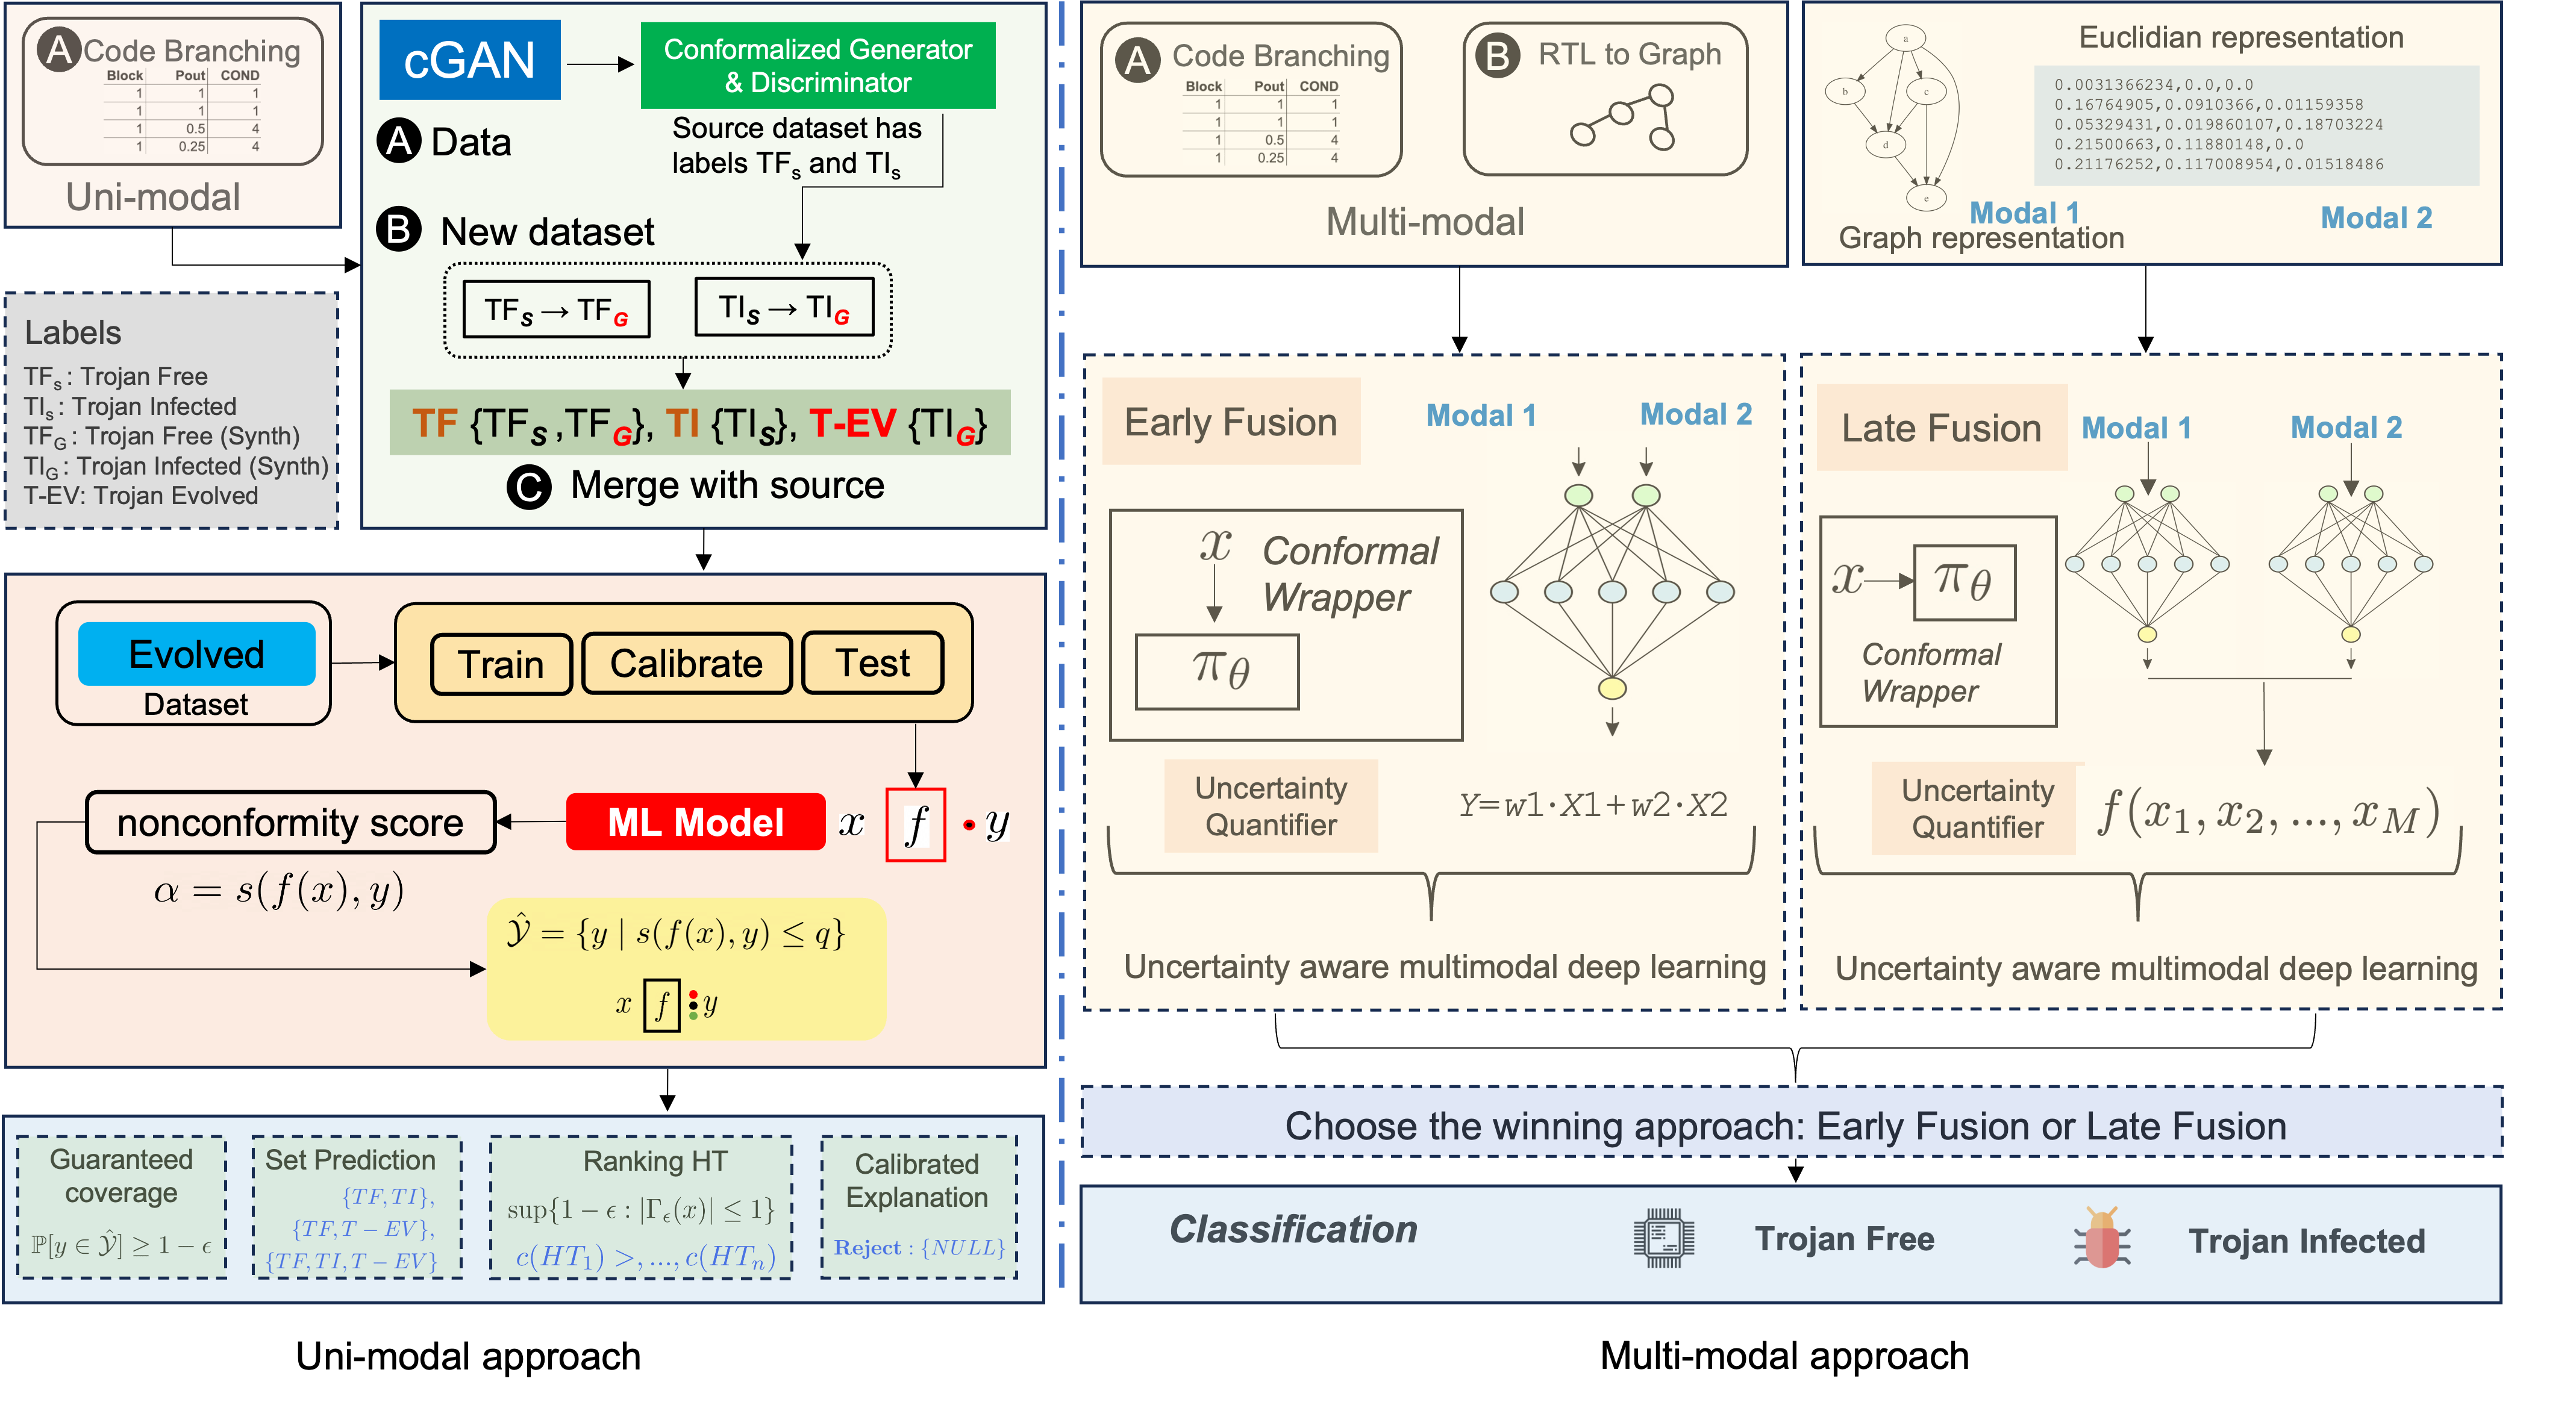
\includegraphics[width=1\linewidth]{figs/solution_thesis.png}
   \caption{The input feature is passed to a conventional machine learning hardware Trojan detector. This detector produces a result and is compared to conformal inference, which provides an uncertainty measure and a confidence set for each detected evolved hardware Trojan.}
  \label{fig:introduction}
\end{figure}
\fi 



\section*{Preliminaries}
\label{Sec:Prelem}
%Background 

%%%%%%%%%%%%%%%%%%%%%%%%%%%%%%%%%%%%%%%%%%%%%%%%%%%%%
    %Calibration
%%%%%%%%%%%%%%%%%%%%%%%%%%%%%%%%%%%%%%%%%%%%%%%%%%%%%
\subsection*{Calibrated Prediction}
\label{sec:Calibration}
Calibration involves ensuring that a model's confidence score accurately reflects the true probability of the prediction's correctness \cite{ovadia2019can}. Let $X$ be the input data, and $Y$ be the output label. Given a training dataset $D = {(x_1, y_1), (x_2, y_2),..., (x_n, y_n)}$, the goal is to learn a function $f$ that can predict the correct output label $y$ for a given input $x$. The output of the model for an input $x$ can be denoted as $f(x)$, and the true probability of the prediction's correctness can be denoted as $P(y=1|x)$. A calibrated model produces a confidence score $g(x)$ that reflects the true probability of correctness of the prediction. The goal of calibration is to ensure that the confidence score $g(x)$ is well-calibrated, i.e., $P(y=1|g(x)=p) = p$ for all $p$ in the range $[0, 1]$.

\textbf{Why we need calibration?}

Calibration is a crucial aspect in HT detection since it aids in determining the likelihood of the existence of a Trojan in a circuit, which can have a significant impact on decision-making. In situations where a model's confidence score is high, but the likelihood of a Trojan's presence is low, it is reasonable to assume that the circuit does not contain a Trojan. Conversely, if the confidence score is low but the likelihood of a Trojan's presence is high, further investigation of the circuit is necessary.

%%%%%%%%%%%%%%%%%%%%%%%%%%%%%%%%%%%%%%%%%%%%%%%%%%%%%
    %Conformal Prediction
%%%%%%%%%%%%%%%%%%%%%%%%%%%%%%%%%%%%%%%%%%%%%%%%%%%%%
\subsection*{Conformal Prediction}
\label{sec:CP}
%Conformal prediction is a framework for constructing prediction intervals that are guaranteed to have a specified level of coverage probability, typically at a confidence level of $1-\alpha$ for some pre-specified $\alpha \in (0,1)$. Given a training set ${(X_test, y_test)}{i=1}^n$, where $x_i \in \mathcal{X}$ is a feature vector and $y_i \in \mathcal{Y}$ is a label, the goal is to construct a function $f: \mathcal{X} \rightarrow \mathcal{Y}$ that predicts the label $y$ for a given feature vector $x$. Conformal prediction produces prediction sets $\Gamma(x)$ for a new feature vector $x$ such that $P(y \in \Gamma(x) | x, {(x_i, y_i)}{i=1}^n) \geq 1 - \alpha$ for all $x \in \mathcal{X}$ and for all $y \in \mathcal{Y}$, where $P$ is the probability measure. The prediction sets can be constructed using various methods, including the nonconformist algorithm and the transductive conformal prediction algorithm.

Conformal prediction \cite{shafer2008tutorial} is a ML framework that quantifies prediction uncertainty by generating prediction sets. It enhances the inference of traditional models, ensuring reliable validity and enabling confidence estimation for individual predictions. In the context of detecting HTs, label-conditional validity is a vital property when dealing with an imbalanced dataset where label proportions differ significantly. This is particularly relevant since the likelihood of encountering a Trojan on a circuit is generally low. In addition, it is worth noting that minority classes are often disproportionately impacted by errors when label-conditional validity is absent \cite{lofstrom2015bias}. However, this issue can be mitigated by ensuring label-conditional validity, which guarantees that the error rate for even the minority class will eventually converge to the chosen significance level in the long term. Sometimes, conformal prediction may produce uncertain predictions, meaning that prediction sets contain more than one value. This occurs when none of the labels can be rejected at the specified significance level.

When using conformal prediction, the confusion matrix differs slightly from the conventional one due to the unique nature of \textit{prediction sets}, which consist of multiple values rather than a single value. In the case of binary classification, it is essential to consider the number of correctly predicted examples, which have a prediction set containing only the correct label, as well as the number of incorrectly predicted examples, where the prediction set includes only the incorrect label. Additionally, it is important to take into account the number of inconclusive predictions that occur when the prediction set contains both labels, as well as the number of examples with an \textit{empty prediction set}. Furthermore, in some cases, it may be more appropriate to provide a \textit{single value point prediction} instead of a prediction set or interval in a hedged forecast. In such cases, selecting the label with the highest $p$-value is a simple and reasonable option. The point prediction can be hedged by incorporating additional information that describes the uncertainty.


\begin{figure*}[ht]
  \centering
   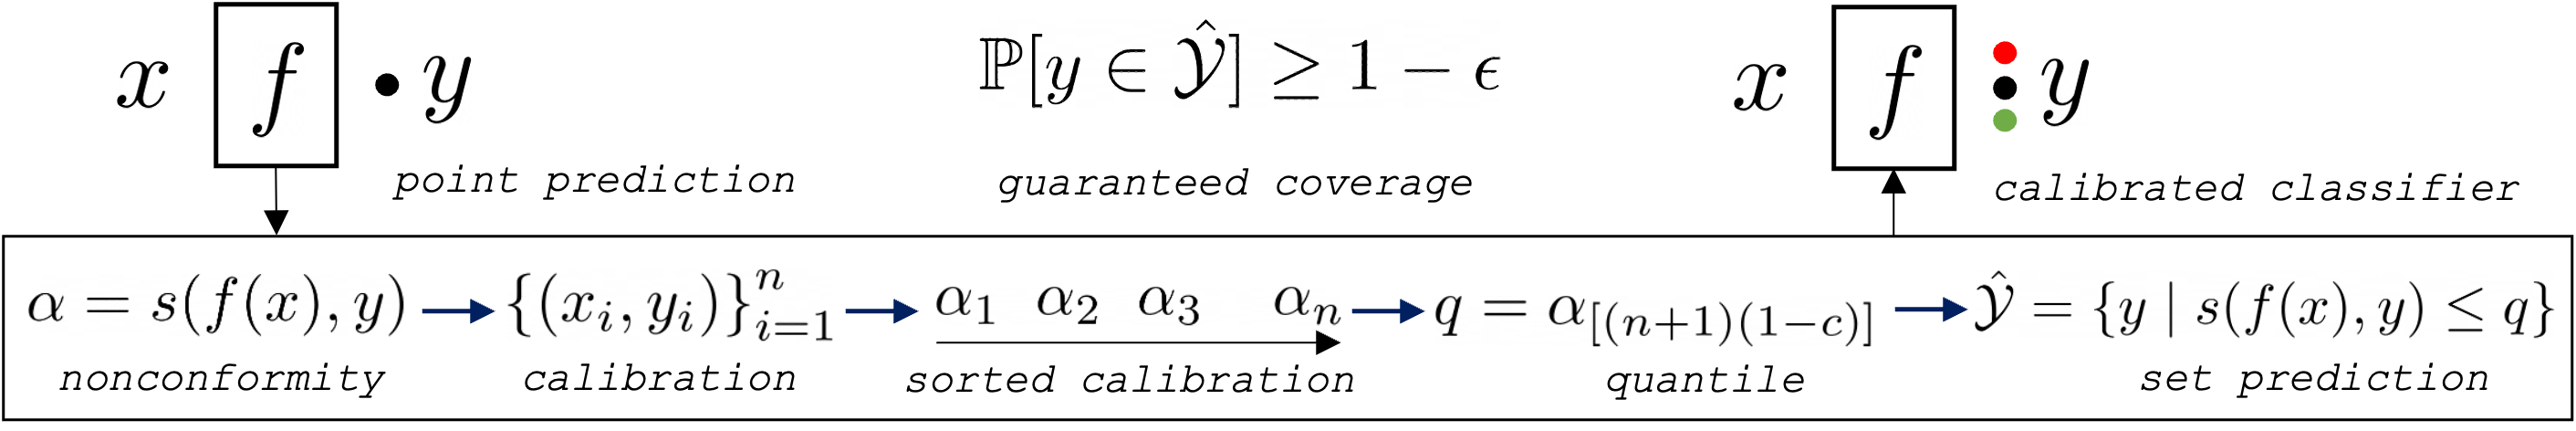
\includegraphics[width=0.95\linewidth]{figs/frameowrk_cp.png}
   \caption{Illustration of Conformal Prediction Framework, showcasing the key components and stages involved in the process.}
  \label{fig:frameowrk_cp}
\end{figure*}


In this thesis our work relies on Mondrian Inductive Conformal Prediction (ICP) \cite{bostrom2021mondrian} as shown in Algorithm \ref{algo:mcp}. Furthermore, to decrease the rate of false negatives in alert systems, we require class-based authenticity for samples classified as "Evolving Trojan". Additionally, we must ensure that the samples labeled as "Evolving Trojan" are indeed genuine to attain this goal.

\begin{algorithm}[t]
\SetKwInOut{Input}{Input}
\SetKwInOut{Output}{Output}
\Input{Training data $D$, test instance $x$, significance level $\alpha$, number of trees $T$, and maximum tree depth $d$.}
\Output{Prediction set $C(x)$ for $x$.}
Divide $D$ into $T$ disjoint subsets $D_1, \ldots, D_T$;

\For{$t \leftarrow 1$ \KwTo $T$}{
Sample $D_t'$ from $D_t$ by recursively partitioning $D_t$ along randomly chosen hyperplanes until each partition contains at most $2d$ points.

Train a classification model $M_t$ on $D_t'$.
}
Compute the conformity scores $s_t(x)$ of $x$ with respect to each model $M_t$.

Sort the conformity scores $s_t(x)$ in decreasing order.

Compute the $p$-values $p_t$ of the $T$ conformity scores $s_t(x)$ using the formula $p_t = \frac{T - t + 1}{T}$.

Compute the threshold $h$ such that $h = s_t(x)$ if $p_t > \alpha$, otherwise $h = \infty$.

Construct the prediction set $C(x)$ as the set of all labels $y$ such that $s_t(y) \geq h$ for all models $M_t$.

\Return $C(x)$
\caption{Mondrian ICP}
\label{algo:mcp}
\end{algorithm}

When calculating the non-conformity scores, we only consider the scores related to the examples that share the same class as the object $x_{n+1}$, which we are testing hypothetically as shown below: 
$$
p_{n+1}^{C_k}=\frac{\left|\left\{i \in 1, \ldots, q: y_i=C_k, \alpha_{n+1}^{C_k} \leq \alpha_i\right\}\right|}{\left|\left\{i \in 1, \ldots, q: y_i=C_k\right\}\right|}
$$


%%%%%%%%%%%%%%%%%%%%%%%%%%%%%%%%%%%%%%%%%%%%%%%%%%%%%
    %Coverage guarantee
%%%%%%%%%%%%%%%%%%%%%%%%%%%%%%%%%%%%%%%%%%%%%%%%%%%%%
\subsection*{Guaranteed Coverage of Prediction}
\label{sec:Coverage}
In the domain of HT detection, it is not only important to have a high level of confidence in the predictions made by a model but also a guarantee of the coverage of each prediction. The property of guaranteed coverage is an inherent property of conformal prediction, which provides statistical guarantees of the correctness of the model's predictions \cite{angelopoulos2023conformal}. The theoretical guarantee of coverage is based on the significance level, which is the probability of the model making a mistake. For example, if we set the significance level to $0.05$, it means that we allow the model to make mistakes $5\%$ of the time.

%Let $X$ be the input data and $Y$ be the output label. Given a training dataset $D = {(x_1, y_1), (x_2, y_2),..., (x_n, y_n)}$, the goal is to learn a function $f$ that can predict the correct output label $y$ for a given input $x$.
%The conformal prediction algorithm works by constructing a prediction set for each input $x$ in the test dataset. This prediction set is a set of potential output labels that the model predicts with a high degree of confidence. The size of the prediction set depends on the significance level and the quality of the model. Let $C(x)$ be the prediction set for the input $x$. We provide a mathematical proof of the guaranteed coverage of predictions by conformal prediction. 
The theoretical guarantee of coverage is valid for any input $x$, that the true output label $y$ will be contained in the prediction set $C(x)$ with a probability of at least $1 - \alpha$, where $\alpha$ is the significance level. Mathematically, this can be expressed as:

$$
P(y \in C(x)) \geq 1 - \alpha
$$

In other words, the probability of making a mistake is bounded by $\alpha$, and as $\alpha$ decreases, the size of the prediction set decreases, leading to higher confidence in the model's predictions. Similarly, if the value of $\alpha$ increases, consequently the size of the prediction set also increases; however, this also reduces the significance level (confidence) of the predictions. 

For example, if we set $\alpha = 0.05$, it means that we are $95\%$ confident that the true output label $y$ is contained in the prediction set $C(x)$ for any input $x$. The use of conformal prediction provides a strong theoretical guarantee of the correctness of the model's predictions in the context of HT detection, and the corresponding proof is given in Theorem \ref{thm:coverage}.

\begin{theorem}\label{thm:coverage}
Let $\mathcal{D}$ be a probability distribution over a set $\mathcal{X} \times \{0,1\}$, where $\mathcal{X}$ is a set of input features and $\{0,1\}$ is the set of labels. Let $f: \mathcal{X} \to \{0,1\}$ be a binary classifier, and let $\epsilon \in (0,1)$ be a confidence level. Then, the conformal prediction algorithm outputs a set of predictions $C(x) \subseteq \{0,1\}$ for each input $x \in \mathcal{X}$ such that:

\begin{equation*}
\mathbb{P}[(x,y) \sim \mathcal{D}, y \in C(x)] \geq 1-\epsilon
\end{equation*}

where $(x,y) \sim \mathcal{D}$ denotes sampling a pair $(x,y)$ from the distribution $\mathcal{D}$.

\end{theorem}

\begin{proof}
The proof follows from the construction of the conformal prediction algorithm. Given an input $x$, the algorithm outputs a set of predictions $C(x)$ based on the observed labels of the training examples with similar input features to $x$. The algorithm guarantees that each prediction in $C(x)$ has a $p$-value less than or equal to $\epsilon$ for any new input with the same feature vector as $x$. Since the algorithm outputs a set of predictions, the probability that at least one of the predictions is correct is at least $1-\epsilon$. 
\end{proof}

\begin{corollary}\label{cor:coverage}
Let $\mathcal{D}$, $f$, and $\epsilon$ be as in Theorem~\ref{thm:coverage}. For any sample size $n$, the conformal prediction algorithm outputs a set of predictions $C(x_1),\ldots,C(x_n)$ for each input $x_1,\ldots,x_n \in \mathcal{X}$ such that:

\begin{equation*}
\mathbb{P}[\forall i \in \{1,\ldots,n\}, (x_i,y_i) \sim \mathcal{D}, y_i \in C(x_i)] \geq 1-\epsilon
\end{equation*}

where $(x_i,y_i) \sim \mathcal{D}$ denotes sampling a pair $(x_i,y_i)$ from the distribution $\mathcal{D}$ for each $i$.

\end{corollary}

\begin{proof}
The proof follows from a union bound over the $n$ samples:

\begin{equation*}
\begin{aligned}
&\mathbb{P}[\forall i \in \{1,\ldots,n\}, (x_i,y_i) \sim \mathcal{D}, y_i \in C(x_i)] \\
&\geq 1 - \sum_{i=1}^n \mathbb{P}[(x_i, y_i) \sim \mathcal{D}, y_i \notin C(x_i)] \\
&\geq 1 - n \epsilon
\end{aligned}
\end{equation*}

where the second inequality follows from Theorem~\ref{thm:coverage}. 
\end{proof}


\subsection*{Multimodal Learning}
\label{sec:multimodal}
Multimodal learning \cite{ngiam2011multimodal} addresses complex problems by integrating information from multiple modalities, such as text, images, and audio, to obtain a comprehensive understanding of a given phenomenon. In our case, we use graphical data and tabular representations of the source circuits. This approach enables models to capture nuanced relationships that may be overlooked when considering each modality in isolation, and thus empowers the model to make more robust predictions.

From a mathematical perspective, multimodal learning involves the integration of data representations into a unified framework. Let \(X_1, X_2, ..., X_M\) represent \(M\) different modalities of data, each with their respective feature spaces \(\mathcal{F}_1, \mathcal{F}_2, ..., \mathcal{F}_M\). The task is to learn a mapping \(f\) that captures the relationships between these modalities. Mathematically, this can be formulated as:
\begin{equation}
f: \mathcal{F}_1 \times \mathcal{F}_2 \times ... \times \mathcal{F}_M \rightarrow \mathcal{Y}
\end{equation}
where \(\mathcal{Y}\) is the target space, representing the desired prediction.

The challenge lies in effectively combining information from diverse modalities, which can be approached through various techniques such as late fusion or early fusion. 

In late fusion \cite{trong2020late}, features are extracted independently from each modality and then combined at a later stage. This approach treats modalities as separate entities until a decision needs to be made and can be represented as:
\begin{equation}
f(x_1, x_2, ..., x_M) = g(h_1(x_1), h_2(x_2), ..., h_M(x_M))
\end{equation}
where \(h_i\) represents feature extraction for modality \(i\), and \(g\) combines the extracted features.

In early fusion \cite{nguyen2021gefa}, information from different modalities is combined at the input level, resulting in a joint feature representation which can be expressed as:
\begin{equation}
f(x_1, x_2, ..., x_M) = h(x_1, x_2, ..., x_M)
\end{equation}
where \(h\) combines the raw input data from all modalities.

\section*{Related Works}
\label{Related}
HT detection using traditional ML techniques has primarily focused on modeling methods, and it involves developing and implementing algorithms that can improve overall accuracy in detecting HTs. The input to the model consists of the features extracted from the Register Transfer Level (RTL) code as tabular and graphical representations of the circuit. Different surveys on ML for detecting HT attacks have been conducted in \cite{huang2020survey}, \cite{gubbi2023hardware}, \cite{koylu2023survey}, and \cite{kundu2021application}. In \cite{botero2021hardware} and \cite{ashok2022hardware} image classification is used, and in \cite{10027082} multimodal image processing is utilized. Most of the papers have focused on feature extraction from gate-level netlists and using ML models such as Support Vector Machine (SVM) \cite{bao2014application}, Neural Network (NN) \cite{hasegawa2017hardware}, eXtreme Gradient Boosting (XGB) \cite{dong2019machine}, and Random Forest (RF) classifier \cite{hasegawa2017trojan}.

% RL
With the success of Reinforcement Learning (RL) in other domains, a few works have adapted RL in the hardware security domain, such as RL-based static detection \cite{gohil2022attrition}, and RL with adaptive sampling for on-chip detection \cite{chen2023adatest}. In these methods, a common approach involves training the classifier model initially and then adjusting the hyperparameters of the classifier. This adjustment process aims to minimize the false negative rate and, in turn, improve the model's accuracy. Graph Neural Network (GNN) \cite{alrahis2022embracing,hepp2022golden} and Abstract Syntax Tree (AST) \cite{han2019hardware} are generated for the RTL code; however, it is still not clear how the graphs can carry forward not only the structural but also the behavioral attributes of the circuit.

% Drift 
Furthermore, dealing with concept drift is crucial after deploying a model because the newly acquired data can be significantly dissimilar to the data the model was originally trained on. One such work in security applications is shown in \cite{yang2021cade} which involves the mapping of data samples into a space with fewer dimensions and the automatic learning of a distance function that can evaluate the differences between them. The concept drift, however, has not been studied in the HT domain even though HTs can evolve over time.

% Explainability 
The explainability aspect of ML is also covered in the hardware security domain; for example, \cite{pan2023hardware}, \cite{downing2021deepreflect}, and \cite{severi2021explanation} have used SHapley Additive exPlanations (SHAP) on benchmark datasets and have shown promising results. However, a drawback of utilizing SHAP is that it comes with inherent issues such as disregarding causality and being affected by human bias. It merely assesses the extent to which features contribute to a given dataset, without providing an explanation of how they would behave in the actual world, which may differ from the dataset used.

The emphasis in traditional ML approaches for HT detection has primarily been on modeling techniques. This entails the development and implementation of algorithms aimed at enhancing the overall accuracy of HT detection. The model takes as input features extracted from the Register Transfer Level (RTL) code, which are represented both in tabular and graphical forms depicting the circuit. Various surveys on the application of ML in detecting HT attacks have been conducted.  
Many research papers have concentrated on extracting features from Register Transfer Level (RTL) or gate-level netlists and employing ML models such as Support Vector Machine (SVM) \cite{bao2014application}, Neural Network (NN) \cite{hasegawa2017hardware}, eXtreme Gradient Boosting (XGB) \cite{dong2019machine}, and the Random Forest (RF) classifier \cite{hasegawa2017trojan}. In \cite{ashok2022hardware}, image classification techniques are also employed. %while in \cite{10027082}, a multimodal image processing approach is utilized, the only paper that detects HTs using multimodal image processing.

Multimodal Deep Learning (DL) has been a well-explored topic in the Artificial Intelligence (AI) community. Early research, exemplified by Deep Boltzmann Machines (DBM) focused on the model's capacity to understand probability distributions across inputs with multiple modes \cite{srivastava2012multimodal}. Additionally, applications of uncertainty-aware multimodal learning \cite{wang2022uncertaintyaware} have been successfully demonstrated in healthcare \cite{sarawgi2021uncertainty} and in scenarios involving multimodal task distributions \cite{almecija2022uncertaintyaware}, particularly in safety-critical environments. In our work, we target the fusion of graph \cite{ektefaie2023multimodal, kim2023heterogeneous} and Euclidean data as the modalities of interest along with uncertainty estimation. 

Moreover, when working in the hardware security domain, it is expected to have fewer data points that are malicious or Trojan-infected. In this context, it is necessary to work with small data \cite{nyiri2023can} and this has been achieved in various domains such as material science \cite{xu2023small} and anomaly detection \cite{ghamisi2023anomaly}.

\section*{Contributions}
\label{Contribution}
In this thesis, our primary focus revolves around multimodal deep learning for the identification of hardware trojans, and addressing the inherent challenges associated with this problem, for example, missing modalities and imbalanced dataset. The first challenge pertains to effectively handling missing modalities and implementing uncertainty-aware multimodal fusion approaches. To address this, we utilize graphical representations of circuits \cite{yu2021hw2vec} and Euclidean data derived from processing the Abstract Syntax Tree (AST) of RTL files (Verilog) \cite{px6s-sm21-22}. While multimodal approaches have been employed to enhance model accuracy in various domains, their application in Trojan identification has been notably absent. For uncertainty-aware multimodal learning, we advocate for implementing logic at the information fusion level of modalities, leveraging $p$-values aggregation with conformal prediction.

The second challenge we tackle is the quantification of uncertainty associated with hardware trojan prediction outcomes and ensuring the validity of predicted labels, especially when dealing with a limited number of highly imbalanced data points. Specifically, our interest lies in the ability of a machine learning classifier to predict the true label of a new data point with a 95\% provable guaranteed coverage, a crucial requirement in risk-sensitive domains. Designing such a system holds potential benefits for decision-makers investigating detected labels as "Trojan-Infected." Additionally, we explore the possibility of ranking detected "Trojan-Infected" circuits to enable more informed treatment decisions.

Our primary contributions are summarized as follows:

\begin{itemize}
\item Proposing a \textbf{multimodal learning approach using graph and euclidean data} of the hardware circuits. This study is the first to investigate and implement a multimodal approach for HT detection, emphasizing uncertainty-awareness.
\item Suggesting a \textbf{model fusion approach that leverages $p$-values as statistical measures}, systematically assessing each modality's contribution to the overall prediction. This enhances interpretability and facilitates more robust decision-making.
\item Addressing the \textbf{challenges of missing modalities} and solving the issue of handling an imbalanced and small dataset by leveraging generative adversarial networks. Introducing the notion of HT evolution and providing an innovative method of creating evolving HTs with high precision using a conformalized generative adversarial network.
\item Novel concept of \textbf{guaranteed coverage of the prediction set}, proposing a tunable significance level through conformal prediction for HT detection. Additionally, defining an algorithm-agnostic and explainability-aware reject prediction made by the ML model. When the model is uncertain about identifying the evolving Trojan, it rejects the prediction, passing it to a human for manual investigation.
\item Proposing a \textbf{ranking mechanism for the evolved Trojans} by assigning a confidence score from the prediction. This contribution is validated on synthetic and real chip-level HT-induced benchmarks.
\end{itemize}


\endgroup
\newpage

\phantomsection
\addcontentsline{toc}{section}{2. DETECTING EVOLVING HARDWARE TROJANS}
\section*{Chapter 2 \\ DETECTING EVOLVING HARDWARE TROJANS}
\begingroup
\RaggedRight

\begin{quote}
"The scientist has a lot of experience with ignorance and doubt and uncertainty, and this experience is of very great importance, I think. When a scientist doesn't know the answer to a problem, he is ignorant. When he has a hunch as to what the result is, he is uncertain. And when he is pretty damn sure of what the result is going to be, he is still in some doubt. Scientific knowledge is a body of statements of varying degrees of certainty -- some most unsure, some nearly sure, but none absolutely certain."
\newline
\hfill — \textit{Richard Feynman}
\end{quote}

\section*{Introduction}
\label{Intro}
Hardware Trojan (HT) insertion is a malicious modification made to the design of a hardware component that can cause a device to malfunction, leak sensitive information, or even cause physical damage \cite{francq2015introduction}. As the semiconductor industry has been adopted a fabless model, the possibility of HTs being inserted at different manufacturing stages increases, presenting a significant security threat to hardware systems. Traditional HT detection techniques such as signature-based methods \cite{gbade2014signature} that analyze the Integrated Circuit (IC) functionality, layout, and timing, are often ineffective against sophisticated HT insertion attacks, especially when the Trojans can be designed to evolve over time. Therefore, there has been a growing shift towards the use of Machine Learning (ML)-based solutions for a more effective and efficient approach to detecting HTs. However, even after adhering to the ML evaluation best practices, it may backfire in the context of hardware security \cite{285613}. The majority of the existing ML-based solutions do not provide enough information on the dataset, where the distribution between classes differs substantially, and the evaluation of attacks under the concept drift or evolution of new incoming dataset. In this context, a detailed study has been conducted in \cite{quiring2022and} to understand if ML is the silver bullet for each and every problem in hardware security domain \cite{liu2021two}.

When using any ML method, one problem that we foresee is that even if a model claims to have a very small false positive rate, there is no guarantee that the same will be applicable for unseen data. This is due to concept drift, which is caused by the attacker's intelligently modified version of HT insertion techniques. One missed false positive can have not only a significant financial and economic impact but can also be life-threatening in high-risk, sensitive domains, such as implantable devices. Therefore, there is a need for additional metrics that can complement the existing model evaluation techniques, provide reliable decisions, and guarantee coverage for the predictions. In this work, we propose \textbf{PALETTE}, an ex\textbf{P}lainable fr\textbf{A}mework for evo\textbf{L}ving hardwar\textbf{E} \textbf{T}rojan de\textbf{TE}ction in risk-sensitive domains based on the algorithm-agnostic statistical inference technique of conformal prediction \cite{shafer2008tutorial} and provide risk-aware theoretical guaranteed coverage of predictions valid under covariate shift \cite{tibshirani2019conformal}. Our method is non-invasive which can be applied as a wrapper over existing ML models. In addition, rather than simply providing a point prediction, i.e., the detected circuit is infected with Trojan or not, it provides a set prediction of the detected labels resulting in the correct class being included 95\% of the time on average (i.e., $\alpha$ = 0.05).

\begin{figure*}[ht]
  \centering
   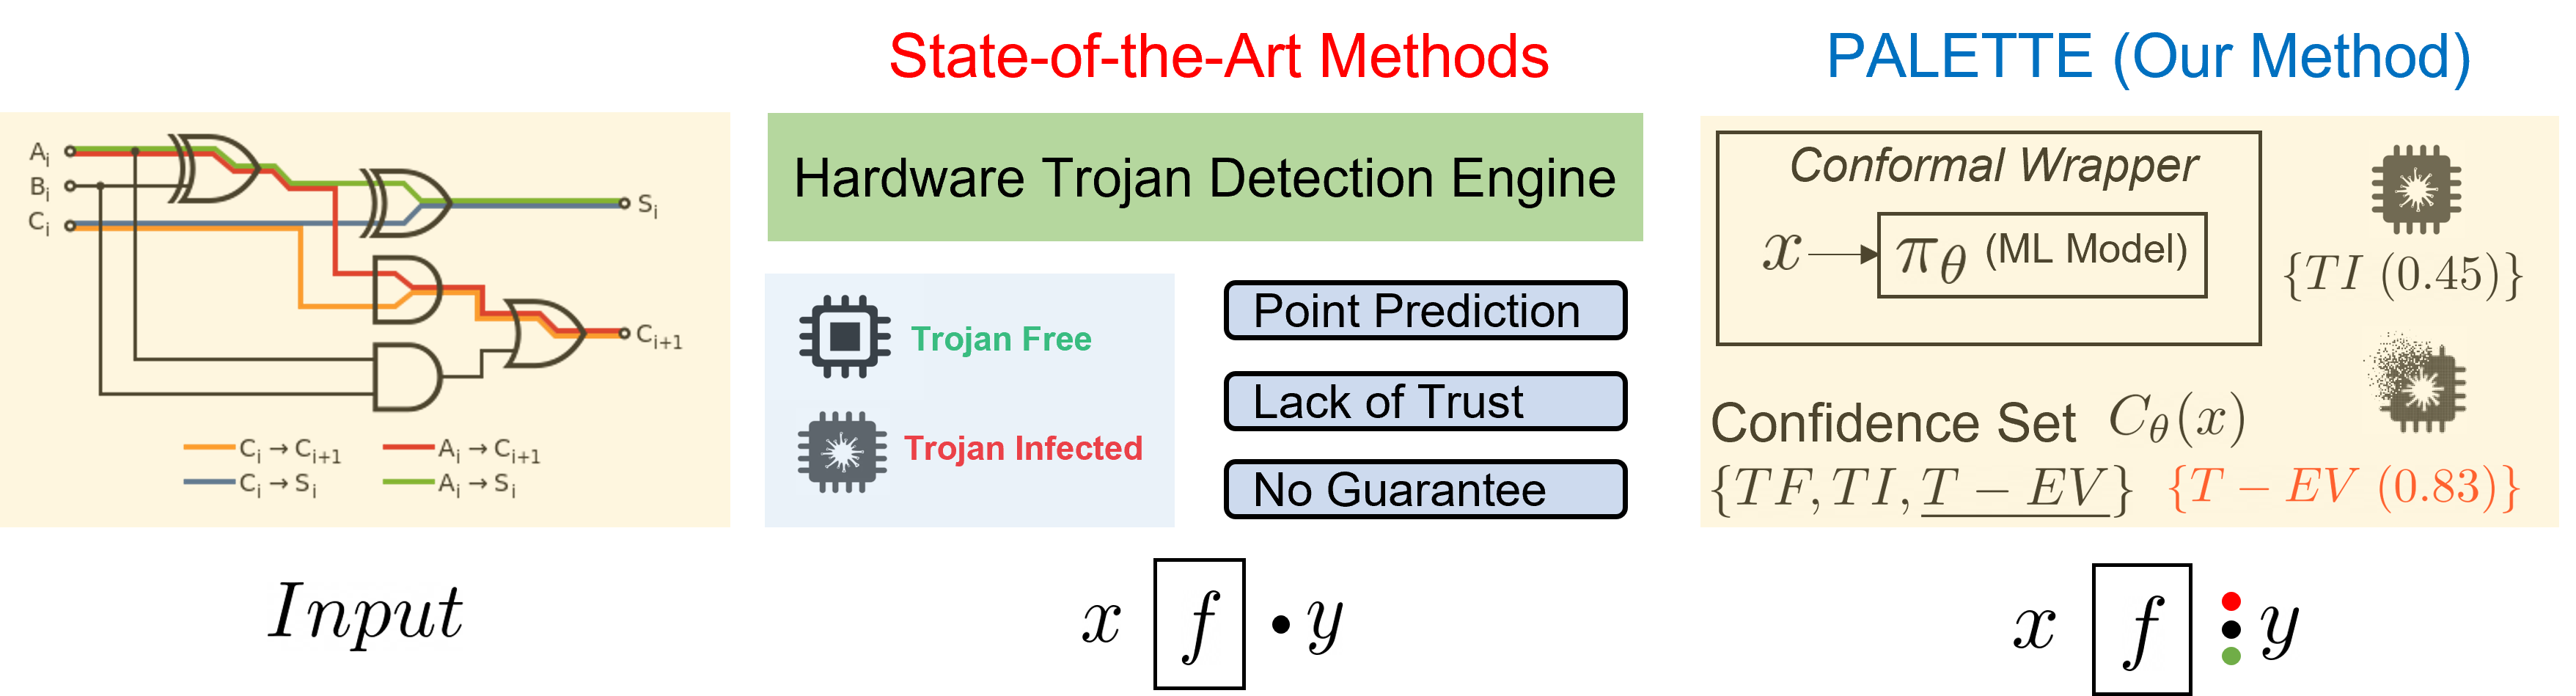
\includegraphics[width=0.95\linewidth]{figs/Intro3.png}
   \caption{The input feature is passed to a conventional machine learning hardware Trojan detector. This detector produces a result and is compared to conformal inference, which provides an uncertainty measure and a confidence set for each detected evolved hardware Trojan.}
  \label{fig:intro}
\end{figure*}


In this paper, we pave the way for hardware security researchers to apply ML to their problems and create awareness about risk-controlled predictions with guaranteed coverage.
% \section{Introduction}
% \label{sec:introduction}
% The semiconductor industry's transition to a fabless manufacturing model has introduced significant security challenges, notably in the form of hardware Trojans (HTs). These malicious modifications, inserted during various production stages, pose risks such as information leakage, device malfunction, and even physical damage. Traditional HT detection methods have been increasingly challenged by the evolving sophistication of these threats \cite{salmani2017hardware, Regazzoni:HTDetection, Guin:HTDetection, Salmani:HTDetection}.

% In response, machine learning (ML) has emerged as a potent tool for HT detection, capitalizing on its ability to discern complex patterns indicative of Trojans \cite{gubbi2023hardware, huang2020survey, liakos2019machine}. However, the reliance on ML solutions is not without its challenges, especially in high-stakes domains where the margin for error is minimal. The inherent limitations of ML models, coupled with the dynamic nature of HTs, demand more adaptive and reliable detection methods \cite{koblah2023survey, koylu2023survey}.

% Addressing this need, our paper introduces a novel approach that synergizes the capabilities of generative adversarial networks (GANs) and statistical inference frameworks. We propose the use of conformalized generative adversarial networks for the generation and simulation of evolving HTs, providing a testbed that closely resembles real-world conditions \cite{ngiam2011multimodal, srivastava2012multimodal}. This is augmented with a Mondrian conformal predictor-based statistical inference framework, serving as a non-invasive wrapper over existing ML models \cite{vovk2016criteria, shafer2008tutorial}. This framework not only offers set predictions for newly detected Trojans but also quantifies uncertainty, enabling more informed decision-making \cite{angelopoulos2023conformal, bostrom2021mondrian}.

% A key feature of our approach is its calibrated explainability mechanism, which comes into play when faced with uncertain or null set predictions. This ability to reject decisions when necessary is critical for maintaining high standards of reliability and trustworthiness in HT detection \cite{li2022interpretable, caruana2020intelligible}.

% Our method's efficacy is validated through extensive evaluations on both synthetic and real-world chip-level benchmarks, demonstrating its potential as a robust solution in the realm of hardware security \cite{10027082, wang2022uncertaintyaware}.

\subsection*{Related Works}
\label{Related}
HT detection using traditional ML techniques has primarily focused on modeling methods, and it involves developing and implementing algorithms that can improve overall accuracy in detecting HTs. The input to the model consists of the features extracted from the Register Transfer Level (RTL) code as tabular and graphical representations of the circuit. Different surveys on ML for detecting HT attacks have been conducted in \cite{huang2020survey}, \cite{gubbi2023hardware}, \cite{koylu2023survey}, and \cite{kundu2021application}. In \cite{botero2021hardware} and \cite{ashok2022hardware} image classification is used, and in \cite{10027082} multimodal image processing is utilized. Most of the papers have focused on feature extraction from gate-level netlists and using ML models such as Support Vector Machine (SVM) \cite{bao2014application}, Neural Network (NN) \cite{hasegawa2017hardware}, eXtreme Gradient Boosting (XGB) \cite{dong2019machine}, and Random Forest (RF) classifier \cite{hasegawa2017trojan}.

% RL
With the success of Reinforcement Learning (RL) in other domains, a few works have adapted RL in the hardware security domain, such as RL-based static detection \cite{gohil2022attrition}, and RL with adaptive sampling for on-chip detection \cite{chen2023adatest}. In these methods, a common approach involves training the classifier model initially and then adjusting the hyperparameters of the classifier. This adjustment process aims to minimize the false negative rate and, in turn, improve the model's accuracy. Graph Neural Network (GNN) \cite{alrahis2022embracing,hepp2022golden} and Abstract Syntax Tree (AST) \cite{han2019hardware} are generated for the RTL code; however, it is still not clear how the graphs can carry forward not only the structural but also the behavioral attributes of the circuit.

% Drift 
Furthermore, dealing with concept drift is crucial after deploying a model because the newly acquired data can be significantly dissimilar to the data the model was originally trained on. One such work in security applications is shown in \cite{yang2021cade} which involves the mapping of data samples into a space with fewer dimensions and the automatic learning of a distance function that can evaluate the differences between them. The concept drift, however, has not been studied in the HT domain even though HTs can evolve over time.

% Explainability 
The explainability aspect of ML is also covered in the hardware security domain; for example, \cite{pan2023hardware}, \cite{downing2021deepreflect}, and \cite{severi2021explanation} have used SHapley Additive exPlanations (SHAP) on benchmark datasets and have shown promising results. However, a drawback of utilizing SHAP is that it comes with inherent issues such as disregarding causality and being affected by human bias. It merely assesses the extent to which features contribute to a given dataset, without providing an explanation of how they would behave in the actual world, which may differ from the dataset used.

\subsection*{Contributions}
\label{Contribution}
In this paper, we answer two questions. First, \textit{can we quantify the uncertainty associated with the HT prediction outcome and guarantee the validity of the predicted label with a handful of highly imbalanced data points? } Specifically, we are interested in the possibility that a ML classifier can predict the truth label of a new data point with 95\% provable guaranteed coverage, which is required in a risk-sensitive domain. Designing such a system can be beneficial to the decision maker who is going to investigate if the detected label is ``Trojan-Infected''. Second, \textit{can we rank the detected ``Trojan-Infected'' circuit for more informed treatment?} Answering this question will help the designer prioritize which one to take action on first for mitigation.

The big picture of our method compared with state-of-the-art ones is shown in Fig. \ref{fig:intro}. In this diagram, we also show the current limitations of using any of the ML frameworks for HT detection. First, they output the prediction as either label-A or label-B; second, there is a lack of trust in the prediction because not all ML classifiers are well calibrated; and third, there is no guarantee of coverage of the predictions. Our main contributions are as follows:

\begin{itemize}
\item Suggesting the notion of \textit{HT evolution} and providing an innovative method of creating evolving HTs with high precision by conformalized generative adversarial network.
\item Discussing the novel notion of \textit{guaranteed coverage} of the prediction set and proposing tunable significance level by leveraging the statistical inference tool of conformal prediction for HT detection.
\item Defining the notion of algorithm-agnostic and explainability-aware \textit{reject prediction} made by the ML model. When the model is uncertain of identifying the evolving Trojan, it simply says, ``I don't know,'' rejecting the prediction and passing it to a human for manual investigation.
\item Proposing a \textit{ranking mechanism} for the evolved Trojans by assigning the confidence score from the prediction and validating the proposed HT detection method both on synthetic and real chip-level HT-induced benchmarks.
\end{itemize}

%\subsection{Organization}
%The rest of the paper is organized as follows. Section \ref{Sec:Prelem} reviews the required preliminary knowledge to conduct this research. Section \ref{sec:Evolution} borrows the notion of evolution from biological science and customizes it for HT detection. Section \ref{sec:Solution} proposes to design evolving Trojans using conformalized generative adversarial networks and uses evolved dataset to make informed, risk-aware predictions with guaranteed coverage. Section \ref{sec:Results} shares the comprehensive experimental results on both synthetic and real chip-level Trojan benchmarks. Finally, Section \ref{Sec:Conclusion} gives the final discussion and conclusion.

\section*{Preliminaries}
\label{Sec:Prelem}
%Background 

%%%%%%%%%%%%%%%%%%%%%%%%%%%%%%%%%%%%%%%%%%%%%%%%%%%%%
    %Calibration
%%%%%%%%%%%%%%%%%%%%%%%%%%%%%%%%%%%%%%%%%%%%%%%%%%%%%
\subsection*{Calibrated Prediction}
\label{sec:Calibration}
Calibration involves ensuring that a model's confidence score accurately reflects the true probability of the prediction's correctness \cite{ovadia2019can}. Let $X$ be the input data, and $Y$ be the output label. Given a training dataset $D = {(x_1, y_1), (x_2, y_2),..., (x_n, y_n)}$, the goal is to learn a function $f$ that can predict the correct output label $y$ for a given input $x$. The output of the model for an input $x$ can be denoted as $f(x)$, and the true probability of the prediction's correctness can be denoted as $P(y=1|x)$. A calibrated model produces a confidence score $g(x)$ that reflects the true probability of correctness of the prediction. The goal of calibration is to ensure that the confidence score $g(x)$ is well-calibrated, i.e., $P(y=1|g(x)=p) = p$ for all $p$ in the range $[0, 1]$.

Calibration is a crucial aspect in HT detection since it aids in determining the likelihood of the existence of a Trojan in a circuit, which can have a significant impact on decision-making. In situations where a model's confidence score is high, but the likelihood of a Trojan's presence is low, it is reasonable to assume that the circuit does not contain a Trojan. Conversely, if the confidence score is low but the likelihood of a Trojan's presence is high, further investigation of the circuit is necessary.

%%%%%%%%%%%%%%%%%%%%%%%%%%%%%%%%%%%%%%%%%%%%%%%%%%%%%
    %Conformal Prediction
%%%%%%%%%%%%%%%%%%%%%%%%%%%%%%%%%%%%%%%%%%%%%%%%%%%%%
\subsection*{Conformal Prediction}
\label{sec:CP}
%Conformal prediction is a framework for constructing prediction intervals that are guaranteed to have a specified level of coverage probability, typically at a confidence level of $1-\alpha$ for some pre-specified $\alpha \in (0,1)$. Given a training set ${(X_test, y_test)}{i=1}^n$, where $x_i \in \mathcal{X}$ is a feature vector and $y_i \in \mathcal{Y}$ is a label, the goal is to construct a function $f: \mathcal{X} \rightarrow \mathcal{Y}$ that predicts the label $y$ for a given feature vector $x$. Conformal prediction produces prediction sets $\Gamma(x)$ for a new feature vector $x$ such that $P(y \in \Gamma(x) | x, {(x_i, y_i)}{i=1}^n) \geq 1 - \alpha$ for all $x \in \mathcal{X}$ and for all $y \in \mathcal{Y}$, where $P$ is the probability measure. The prediction sets can be constructed using various methods, including the nonconformist algorithm and the transductive conformal prediction algorithm.

Conformal prediction \cite{shafer2008tutorial} is a ML framework that quantifies prediction uncertainty by generating prediction sets. It enhances the inference of traditional models, ensuring reliable validity and enabling confidence estimation for individual predictions. In the context of detecting HTs, label-conditional validity is a vital property when dealing with an imbalanced dataset where label proportions differ significantly. This is particularly relevant since the likelihood of encountering a Trojan on a circuit is generally low. In addition, it is worth noting that minority classes are often disproportionately impacted by errors when label-conditional validity is absent \cite{lofstrom2015bias}. However, this issue can be mitigated by ensuring label-conditional validity, which guarantees that the error rate for even the minority class will eventually converge to the chosen significance level in the long term. Sometimes, conformal prediction may produce uncertain predictions, meaning that prediction sets contain more than one value. This occurs when none of the labels can be rejected at the specified significance level.

When using conformal prediction, the confusion matrix differs slightly from the conventional one due to the unique nature of \textit{prediction sets}, which consist of multiple values rather than a single value. In the case of binary classification, it is essential to consider the number of correctly predicted examples, which have a prediction set containing only the correct label, as well as the number of incorrectly predicted examples, where the prediction set includes only the incorrect label. Additionally, it is important to take into account the number of inconclusive predictions that occur when the prediction set contains both labels, as well as the number of examples with an \textit{empty prediction set}. Furthermore, in some cases, it may be more appropriate to provide a \textit{single value point prediction} instead of a prediction set or interval in a hedged forecast. In such cases, selecting the label with the highest $p$-value is a simple and reasonable option. The point prediction can be hedged by incorporating additional information that describes the uncertainty.

Our work relies on Mondrian Inductive Conformal Prediction (ICP) \cite{bostrom2021mondrian} in Algorithm \ref{algo:mcp} and to decrease the rate of false negatives in alert systems, we require class-based authenticity for samples classified as ``Evolving Trojan''. Additionally, we must ensure that the samples labeled as``Evolving Trojan'' are indeed genuine to attain this goal.

\begin{algorithm}[t]
\SetKwInOut{Input}{Input}
\SetKwInOut{Output}{Output}
\Input{Training data $D$, test instance $x$, significance level $\alpha$, number of trees $T$, and maximum tree depth $d$.}
\Output{Prediction set $C(x)$ for $x$.}
Divide $D$ into $T$ disjoint subsets $D_1, \ldots, D_T$;

\For{$t \leftarrow 1$ \KwTo $T$}{
Sample $D_t'$ from $D_t$ by recursively partitioning $D_t$ along randomly chosen hyperplanes until each partition contains at most $2d$ points.

Train a classification model $M_t$ on $D_t'$.
}
Compute the conformity scores $s_t(x)$ of $x$ with respect to each model $M_t$.

Sort the conformity scores $s_t(x)$ in decreasing order.

Compute the $p$-values $p_t$ of the $T$ conformity scores $s_t(x)$ using the formula $p_t = \frac{T - t + 1}{T}$.

Compute the threshold $h$ such that $h = s_t(x)$ if $p_t > \alpha$, otherwise $h = \infty$.

Construct the prediction set $C(x)$ as the set of all labels $y$ such that $s_t(y) \geq h$ for all models $M_t$.

\Return $C(x)$
\caption{Mondrian ICP}
\label{algo:mcp}
\end{algorithm}

When calculating the non-conformity scores, we only consider the scores related to the examples that share the same class as the object $x_{n+1}$, which we are testing hypothetically as shown below: 
$$
p_{n+1}^{C_k}=\frac{\left|\left\{i \in 1, \ldots, q: y_i=C_k, \alpha_{n+1}^{C_k} \leq \alpha_i\right\}\right|}{\left|\left\{i \in 1, \ldots, q: y_i=C_k\right\}\right|}
$$


%%%%%%%%%%%%%%%%%%%%%%%%%%%%%%%%%%%%%%%%%%%%%%%%%%%%%
    %Coverage guarantee
%%%%%%%%%%%%%%%%%%%%%%%%%%%%%%%%%%%%%%%%%%%%%%%%%%%%%
\subsection*{Guaranteed Coverage of Prediction}
\label{sec:Coverage}
In the domain of HT detection, it is not only important to have a high level of confidence in the predictions made by a model but also a guarantee of the coverage of each prediction. The property of guaranteed coverage is an inherent property of conformal prediction, which provides statistical guarantees of the correctness of the model's predictions \cite{angelopoulos2023conformal}. The theoretical guarantee of coverage is based on the significance level, which is the probability of the model making a mistake. For example, if we set the significance level to $0.05$, it means that we allow the model to make mistakes $5\%$ of the time.

%Let $X$ be the input data and $Y$ be the output label. Given a training dataset $D = {(x_1, y_1), (x_2, y_2),..., (x_n, y_n)}$, the goal is to learn a function $f$ that can predict the correct output label $y$ for a given input $x$.
%The conformal prediction algorithm works by constructing a prediction set for each input $x$ in the test dataset. This prediction set is a set of potential output labels that the model predicts with a high degree of confidence. The size of the prediction set depends on the significance level and the quality of the model. Let $C(x)$ be the prediction set for the input $x$. We provide a mathematical proof of the guaranteed coverage of predictions by conformal prediction. 
The theoretical guarantee of coverage is valid for any input $x$, that the true output label $y$ will be contained in the prediction set $C(x)$ with a probability of at least $1 - \alpha$, where $\alpha$ is the significance level. Mathematically, this can be expressed as:

$$
P(y \in C(x)) \geq 1 - \alpha
$$

In other words, the probability of making a mistake is bounded by $\alpha$, and as $\alpha$ decreases, the size of the prediction set decreases, leading to higher confidence in the model's predictions. For example, if we set $\alpha = 0.05$, it means that we are $95\%$ confident that the true output label $y$ is contained in the prediction set $C(x)$ for any input $x$. The use of conformal prediction provides a strong theoretical guarantee of the correctness of the model's predictions in the context of HT detection, and the corresponding proof is given in Theorem \ref{thm:coverage}.

\begin{theorem}\label{thm:coverage}
Let $\mathcal{D}$ be a probability distribution over a set $\mathcal{X} \times \{0,1\}$, where $\mathcal{X}$ is a set of input features and $\{0,1\}$ is the set of labels. Let $f: \mathcal{X} \to \{0,1\}$ be a binary classifier, and let $\epsilon \in (0,1)$ be a confidence level. Then, the conformal prediction algorithm outputs a set of predictions $C(x) \subseteq \{0,1\}$ for each input $x \in \mathcal{X}$ such that:

\begin{equation*}
\mathbb{P}[(x,y) \sim \mathcal{D}, y \in C(x)] \geq 1-\epsilon
\end{equation*}

where $(x,y) \sim \mathcal{D}$ denotes sampling a pair $(x,y)$ from the distribution $\mathcal{D}$.

\end{theorem}

\begin{proof}
The proof follows from the construction of the conformal prediction algorithm. Given an input $x$, the algorithm outputs a set of predictions $C(x)$ based on the observed labels of the training examples with similar input features to $x$. The algorithm guarantees that each prediction in $C(x)$ has a $p$-value less than or equal to $\epsilon$ for any new input with the same feature vector as $x$. Since the algorithm outputs a set of predictions, the probability that at least one of the predictions is correct is at least $1-\epsilon$. 
\end{proof}

\begin{corollary}\label{cor:coverage}
Let $\mathcal{D}$, $f$, and $\epsilon$ be as in Theorem~\ref{thm:coverage}. For any sample size $n$, the conformal prediction algorithm outputs a set of predictions $C(x_1),\ldots,C(x_n)$ for each input $x_1,\ldots,x_n \in \mathcal{X}$ such that:

\begin{equation*}
\mathbb{P}[\forall i \in \{1,\ldots,n\}, (x_i,y_i) \sim \mathcal{D}, y_i \in C(x_i)] \geq 1-\epsilon
\end{equation*}

where $(x_i,y_i) \sim \mathcal{D}$ denotes sampling a pair $(x_i,y_i)$ from the distribution $\mathcal{D}$ for each $i$.

\end{corollary}

\begin{proof}
The proof follows from a union bound over the $n$ samples:

\begin{equation*}
\begin{aligned}
&\mathbb{P}[\forall i \in \{1,\ldots,n\}, (x_i,y_i) \sim \mathcal{D}, y_i \in C(x_i)] \\
&\geq 1 - \sum_{i=1}^n \mathbb{P}[(x_i, y_i) \sim \mathcal{D}, y_i \notin C(x_i)] \\
&\geq 1 - n \epsilon
\end{aligned}
\end{equation*}

where the second inequality follows from Theorem~\ref{thm:coverage}. 
\end{proof}

%%%%%%%%%%%%%%%%%%%%%%%%%%%%%%%%%%%%%%%%%%%%%%%%%%%%%
    %Notion of Evolution
%%%%%%%%%%%%%%%%%%%%%%%%%%%%%%%%%%%%%%%%%%%%%%%%%%%%%
\section*{Notion of Evolution \& Hardware Trojans} 
\label{sec:Evolution}
Darwin, in his book, \textit{On the Origin of Species}, referred to ``descent with modification'', instead of \textit{evolution}. Further, a more expansive definition of evolution was given by Futuyma \cite{laland2014does}: ``biological evolution is change in the properties of groups of organisms over the course of generations; it embraces everything from slight changes in the proportions of different forms of a gene within a population to the alterations that led from the earliest organism to dinosaurs, bees, oaks, and humans''. Now, we narrow down the notion of evolution for HTs based on the following assumptions:

\begin{itemize}
    \item The structural (genotype) and behavioral (phenotype) characteristics of HTs change over a period of time, and the changes are induced by the attacker;
    \item Structural changes can be mathematically formulated for the evolved Trojan as \[ E_{HT} \rightarrow HT \blacksquare HT_{structural\_changes} \] 
    where HT is an existing Trojan and $\blacksquare$ is the operation for structural changes which creates an evolved Trojan $E_{HT}$;
    \item Behavioral changes are mapped with natural selection, which is the driving force for evolution. The attacker designs the HT such that it adapts to the IC (ecosystem) and its malicious impact is not easily detectable on the circuit. (i.e., it increases its chance of survival.)
\end{itemize}

We use the above assumption to include the notion of evolution and derive an evolved dataset in a ML-based HT detection engine. In the context of HTs, we can either detect the evolution or predict the evolution way ahead of time. The detection can be performed using anomaly detection \cite{liu2022anomaly}; however, here we will be focusing on the prediction of evolution. If we can predict the evolutionary changes in the dataset, a specific treatment can be performed to mitigate the impact of HT insertion. To the best of our knowledge, we have not come across any work in the literature that considers the evolutionary aspect while designing HT detection approaches.

%%%%%%%%%%%%%%%%%%%%%%%%%%%%%%%%%%%%%%%%%%%%%%%%%%%%%
    %Designing evolving trojans
%%%%%%%%%%%%%%%%%%%%%%%%%%%%%%%%%%%%%%%%%%%%%%%%%%%%%
%\section{Designing Evolving Hardware Trojans}
%\label{sec:HTDesign}
%Considering, we use any of the above approach and implement machine learning for trojan detection, the first thing we are going to do is to extract the features for the circuit. 
The evolutionary dataset optimization discussed in \cite{edo-paper} optimizes any real-valued function over a subset of the space of all possible datasets. It is not feasible to adapt this method for our use case as our real-time data will be Non-Independent and Identically Distributed (Non-IID). An alternate approach can be to use evolutionary algorithms, as discussed in Box2d \cite{catto2010box2d}. There, the problem statement is to evolve the structure of a toy car, provided the geometry of the car shape is translated to chromosomes. The issue with this approach is that we should know how the evolved car looks; however, in our case, we never know the structure of the evolved Trojan.

\begin{algorithm} [t]
\SetKwInOut{Input}{Input}
\SetKwInOut{Output}{Output}
\Input{Training dataset $\mathcal{D} = \{(x_i, y_i)\}_{i=1}^n$, where $x_i \in \mathbb{R}^p$ and $y_i \in \{0, 1\}$ are the feature vector and label for the $i$-th example, respectively; significance level $\alpha$; number of conformal predictors $M$; GAN generator $G$; discriminator model $D$}
\Output{Conformalized discriminator model $D_\text{CP}$}

\For{$m=1$ \KwTo $M$}{
    $\mathcal{D}_m \gets$ bootstrap sample of $\mathcal{D}$\;
    Train GAN generator $G_m$ on $\mathcal{D}_m$\;
    Generate synthetic dataset $\mathcal{D}_\text{synth}^m = \{G_m(z_i)\}_{i=1}^n$, where $z_i \in \mathbb{R}^k$ are random noise vectors\;
    Train discriminator model $D_m$ on $\mathcal{D}_m \cup \mathcal{D}_\text{synth}^m$\;
}

\For{$i=1$ \KwTo $n$}{
    $X_i \gets \{x_i\} \cup \{G_m(z_i)\}_{m=1}^M$, where $z_i \in \mathbb{R}^k$ are random noise vectors\;
    $\text{CP}_i \gets$ conformal predictor trained on $(X_i, y_i)$ with significance level $\alpha$\;
    $p_i \gets \text{CP}_i(D(x_i))$\;
}

Train conformalized discriminator model $D_\text{CP}$ on $\{(x_i, y_i, p_i)\}_{i=1}^n$\;

For each sample $x_i$ in the test set $D_{test}$, make a prediction based on whether $D(x_i)$ is within the prediction interval $I_i$:
\begin{equation*}
y_i =
\begin{cases}
1 & \text{if } D(x_i) \notin I_i \\
0 & \text{if } D(x_i) \in I_i
\end{cases}
\end{equation*}

\Return{$D_\text{CP}$}

\caption{Conformalized GAN}
\label{alg:cgan1}
\end{algorithm}

\subsection*{Genetic Algorithm} 
\label{sec:GA}
Genetic Algorithms (GAs) \cite{holland1992genetic} have been used to evolve the architecture of NNs for understanding the security of logic locking \cite{sisejkovic2021challenging}. The most challenging part of using GA is designing a fitness function. In our case, one possible design of fitness can focus on the ensemble efficiency of detection methods and then compare the similarity of the child Trojan with the list of HTs in a dictionary. However, the limitation of this fitness function is that it will never be able to estimate the fitness of Trojans that are out of distribution.

\begin{figure*}[ht]
  \centering
   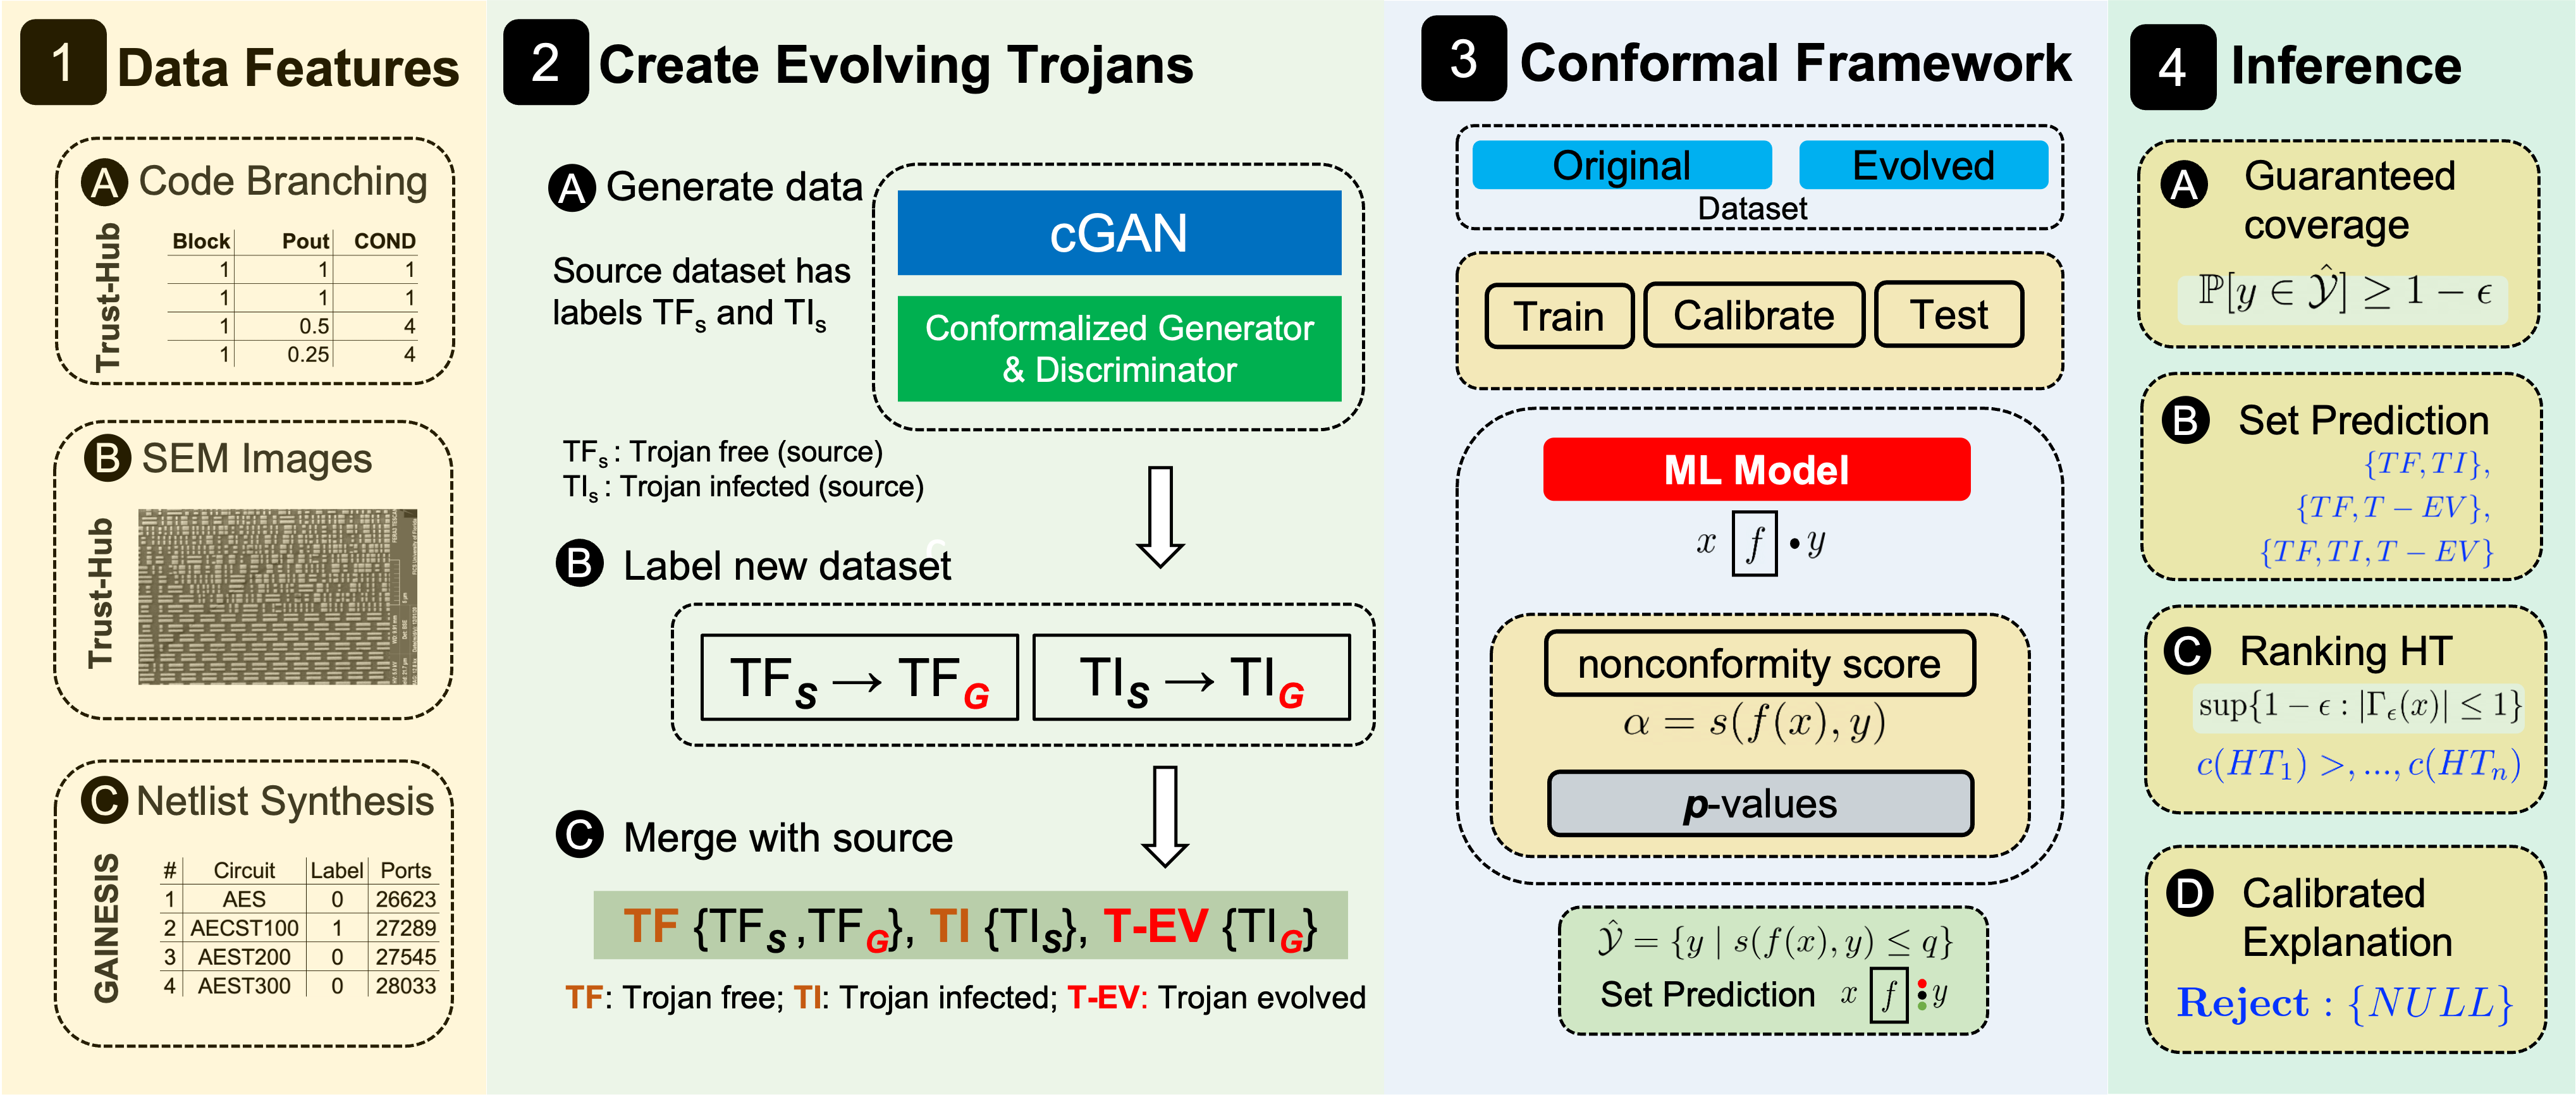
\includegraphics[width=1\linewidth]{figs/Solution.png}
  %\includegraphics[width=\columnwidth]{figs/solution.png}
  \caption{PALETTE: Proposed solution showing the method to design evolving hardware Trojan by tuning conformalized generative adversarial network and using the evolved dataset to make informed, risk-aware predictions with guaranteed coverage.}
  \label{fig:solution}
\end{figure*}

\subsection*{Generative Adversarial Network} 
\label{sec:GAN}
Based on the game theory and optimization approach, the objective of generative modeling \cite{goodfellow2020generative} is to analyze a set of training examples and acquire knowledge about the likelihood distribution that created them. Generative Adversarial Network (GAN) has been successfully used for detecting fake images \cite{ojha2023towards} and text-to-image synthesis \cite{kang2023scaling}. In the recent past, there has been a shift in focus towards the utilization of GANs for working with tabular data. An instance of this approach is used for conditional GAN, as demonstrated by \cite{xu2019modeling}, which models tabular data and is also effective with imbalanced data. %A few of the open source libraries are \cite{ashrapov2020tabular}, \cite{lederrey2022datgan}, and \cite{zhao2023gtv}.

Here are three prime motivations for using GAN for synthesizing the HT dataset. 

\subsubsection*{Highly Imbalanced Data} In a real-time scenario, the labels for Trojan-Infected circuits are very rare and difficult to detect. This gives rise to the problem of an imbalanced dataset. Based on the existing literature, we believe GANs can be used to generate a more realistic synthetic dataset that complements the training phase.

\subsubsection*{Non-IID Case for Law of Large Number} The evolved Trojan may or may not be from the same distribution, and for this reason we have to consider the case of Non-IID random variables. One such an example is demonstrated in \cite{yonetani2019decentralized}. We also know that for a large enough dataset with Non-IID samples, the sample mean will converge to the true population mean as the sample size increases. This implies that as the size of the dataset increases, the statistical properties of the data become more reliable and consistent. Thus, the larger the dataset, the more accurate the model is likely to be, provided that there are enough computational resources to effectively process the data. The proof given in \cite{etemadi1981elementary} for the strong law of large numbers can be generalized to an r-dimensional array of random variables where the sufficient condition becomes $E\left(|X|\left(\log ^{+}|X|\right)^{r-1}\right)<\infty$ based on the theorem and corresponding proof for Non-IID given in \cite{smythe1973strong}. The Non-IID case is worthy of our attention, as evolved HT might not represent the same distribution of population in real-time.

\iffalse 

\begin{theorem}
\label{llm}
The strong law of large numbers for Non-IID random variables states that, if $X_1, X_2, \ldots, X_n$ are a sequence of non-identically distributed random variables with finite means $\mu_1, \mu_2, \ldots, \mu_n$, then for any $\epsilon > 0$,

\begin{equation*}
\mathbb{P} \left( \lim_{n \to \infty} \frac{1}{n} \sum_{i=1}^n (X_i - \mu_i) = 0 \right) = 1 - \sum_{i=1}^n \frac{\mathrm{Var}(X_i)}{n^2 \epsilon^2}.
\end{equation*}

Here, $\mathrm{Var}(X_i)$ denotes the variance of the $i$-th random variable $X_i$.
\end{theorem}

\fi 


\subsubsection*{Risk Sensitive Application} Given the potential for significant financial losses, we cannot afford to tolerate even a small probability of a false positive. To mitigate this, we start by designing a near-realistic synthetic dataset using GAN by conformalizing the discriminator and generator. 


\section*{Designing \& Predicting Evolving Hardware Trojans}
\label{sec:Solution}
Our proposed evolving HT detection method called \textbf{PALETTE} is shown in Fig. \ref{fig:solution} with four major components.

\circleNumber{1} As with any ML-based solution, the first step is to extract the dataset, and in the case of HTs, we can have images, tables, and graphs as input dataset for HT classification. For example, the features extracted from an IC can be Scanning Electron Microscope (SEM) images, as used in \cite{vashistha2018trojan,shi2019golden}. %Very recently, there has been a growing adoption of GNN for HT detection \cite{alrahis2022embracing} by first converting the RTL-level code to AST and then either performing a graph classification or transforming the graph to a vector and then performing the classification. 
In our case, we have used the features extracted based on code branching from the TrustHub chip-level Trojan dataset \cite{px6s-sm21-22} and the netlist synthetic dataset based on GAINESIS \cite{liakos2022gainesis}. 

\circleNumber{2} We introduce the Conformalized GAN algorithm, which is illustrated in Algorithm \ref{alg:cgan1}. Our algorithm is inspired by \cite{sankaranarayanan2022semantic}, which leverages principled uncertainty intervals to generate high-quality images from corrupted inputs, and the uncertainty intervals provide a guarantee of containing the true semantic factors for any underlying generative model. Motivated by their work, we generate high-quality evolved representation of HTs from existing Trust-Hub dataset \cite{px6s-sm21-22} and the netlist synthesis GAINESIS dataset \cite{liakos2022gainesis}. 
The algorithm utilizes conformal prediction to generate evolving HTs and determine its associated level of confidence using prediction intervals. A comparison of Trust-Hub source dataset with the synthetically generated data, which we call the evolved dataset, is shown in Fig. \ref{fig:gan1}. In contrast with traditional GANs our proposed method provides a more reliable means for generating evolving HTs.  

% %%%%%%%%%%%%%%%%%%%%%%
% LIME
% %%%%%%%%%%%%%%%%%%%%%%

\iffalse 

It should be noted that the source dataset has only two labels, i.e., Trojan-Free (TF) and Trojan-Infected (TI), and consequently, the data generated from conformalized GAN also has only two labels. Here, we consider all the data points with label (TI) as Evolved Trojan as they are generated using GAN and this label is assigned T-EV. Finally, a consolidated dataset with evolved HT is created with three labels \{TF, TI, T-EV\}.

\fi 

\begin{figure}[!b]
  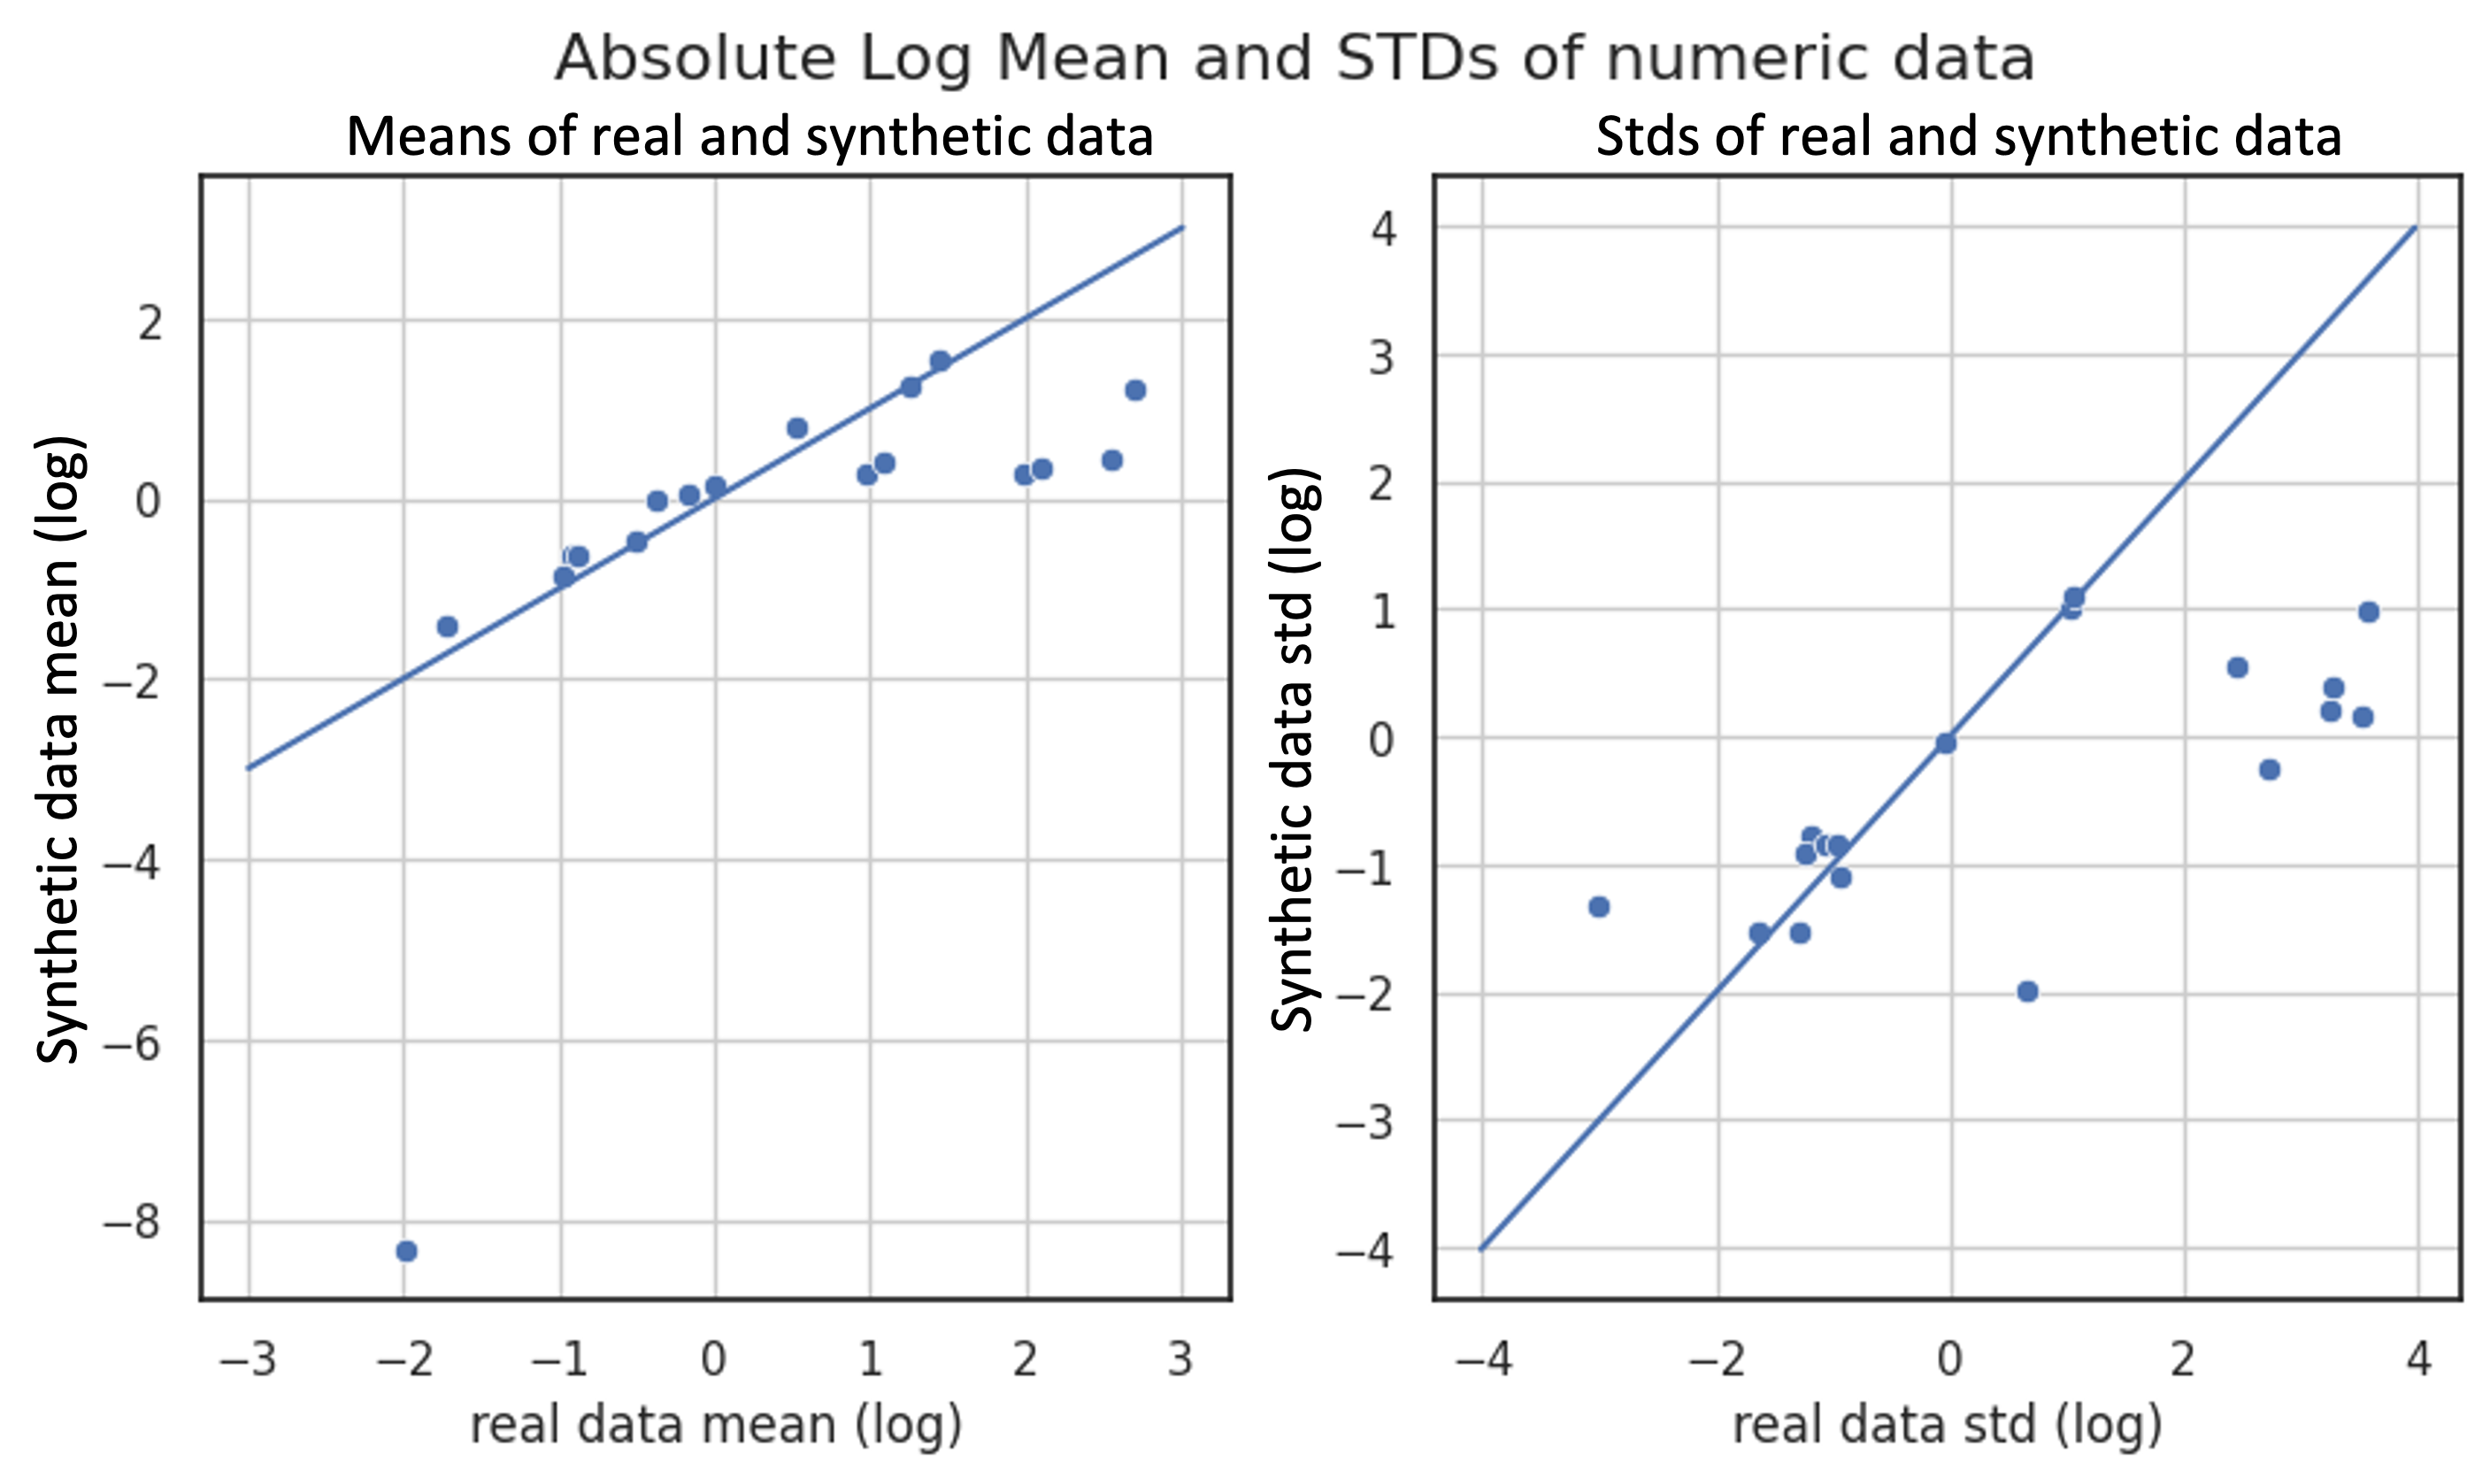
\includegraphics[width=1\linewidth]{figs/gan/real_fake.png}
  \caption{Comparison of real and synthetically generated dataset on Trust-Hub chip-level Trojan dataset.}
  \label{fig:gan1}
\end{figure}

\circleNumber{3} The dataset is further fed as input to the conformal inference engine, which outputs set prediction instead of point predictions based on the significance level. The method is \textit{algorithm-agnostic} as any ML classifier such as statistical or deep learning can be used as shown in Fig. \ref{fig:solution}. The non-conformity score is calculated for each prediction. The $p$-value represents the probability that the prediction is correct and is used to determine the guaranteed coverage. The important part of the solution is how we interpret the results in a risk sensitive domain where we cannot tolerate even a single wrong decision.

\circleNumber{4} We derive four different inferential use cases based on conformal inference. The motive is to quantify the uncertainty associated with each prediction and reduce the False Discovery Rate (FDR) for Trojan-Free (TF), Trojan-Infected (TI), or Evolving Trojan (T-EV). The first is guaranteed coverage, which claims that based on the user-defined significance level, the predicted label will belong to that class. Here, considering the degree of risk associated with the prediction, a significance level is defined and applied to the $p$-values of each label for the data point of the circuit. The second is an inherent property of conformal prediction that results in a set prediction which can have all the labels \{TF, TI, T-EV\}, a combination of labels \{TF, T-EV\} or \{TI, T-EV\}, or a single label \{TF\}, \{TI\}, or \{T-EV\}. The third, ranks the predicted HTs by calculating the confidence of each prediction and using it to rank the severity of being infected with a Trojan (TI, T-EV). The purpose of ranking is to prioritize which one to take action on first for mitigation. Finally, the fourth is calibrated explanation for the predictions where the model says: \textit{``I don't know''} and rejects the prediction. The proposed method overcomes the issues of local explanations by SHAP as discussed in Section \ref{Related} and provides a calibrated approach to reasoning out \textit{``why''} a certain prediction has to be rejected. This is achieved by a \textit{NULL} set, indicating that the model is not able to output the prediction for a specific significance level (1 - $\alpha$). These four risk-aware, tailored prediction use cases are discussed with experimental results in Section \ref{sec:Results}.



%%%%%%%%%%%%%%%%%%%%%%%%%%%%%%%%%%%%%%%%%%%%%%%%%%%%%
   % Experimental results
%%%%%%%%%%%%%%%%%%%%%%%%%%%%%%%%%%%%%%%%%%%%%%%%%%%%%
\section*{Experimental results}
\label{sec:Results}
In this section we share the experimental results on two datasets. First is GAINESIS \cite{liakos2022gainesis} synthetic dataset with binary labels and second is using Trust-Hub chip-level Trojan dataset \cite{px6s-sm21-22}. This dataset includes VHDL or Verilog source code files for each IP core design, which contain both malicious and non-malicious functions. The malicious functions are often embedded within conditional statements that are seldom executed. Consequently, the ML features are extracted from these conditional statements. We used Python (3.9) and implemented the solution on macOS (13.3.1) having 8 GB RAM with built-in GPU. The experimental results with source code and the dataset are hosted on GitHub \footnote{https://github.com/cars-lab-repo/PALETTE/}.

%%%%%%%%%%%%%%%%%%%%%%%%%%%%%%%%%%%%%%%%%%%%%%%%%%%%%
   % Dataset 
%%%%%%%%%%%%%%%%%%%%%%%%%%%%%%%%%%%%%%%%%%%%%%%%%%%%%

\subsection*{Source Dataset}
\label{Sec:Dataset}
For our experiment we have used the features extracted from TrustHub chip-level Trojan dataset based \cite{px6s-sm21-22} on RTL design using \textit{Code branching features}. The dataset includes VHDL or Verilog source code files for each IP core design, which contain both malicious and non-malicious functions. The malicious functions are often embedded within conditional statements that are seldom executed. Consequently, the machine learning features are extracted from these conditional statements. %There are 197 data points in the dataset which are marked as $TI_{S}$ (label = 1) and 901 as $TF_{S}$ (label = 0). 

We also use synthetic dataset from GAINESIS which has two labels \{TF,TI\}. The results are share in the following sections.  


\iffalse 
\begin{figure*}[ht]
  \centering
   %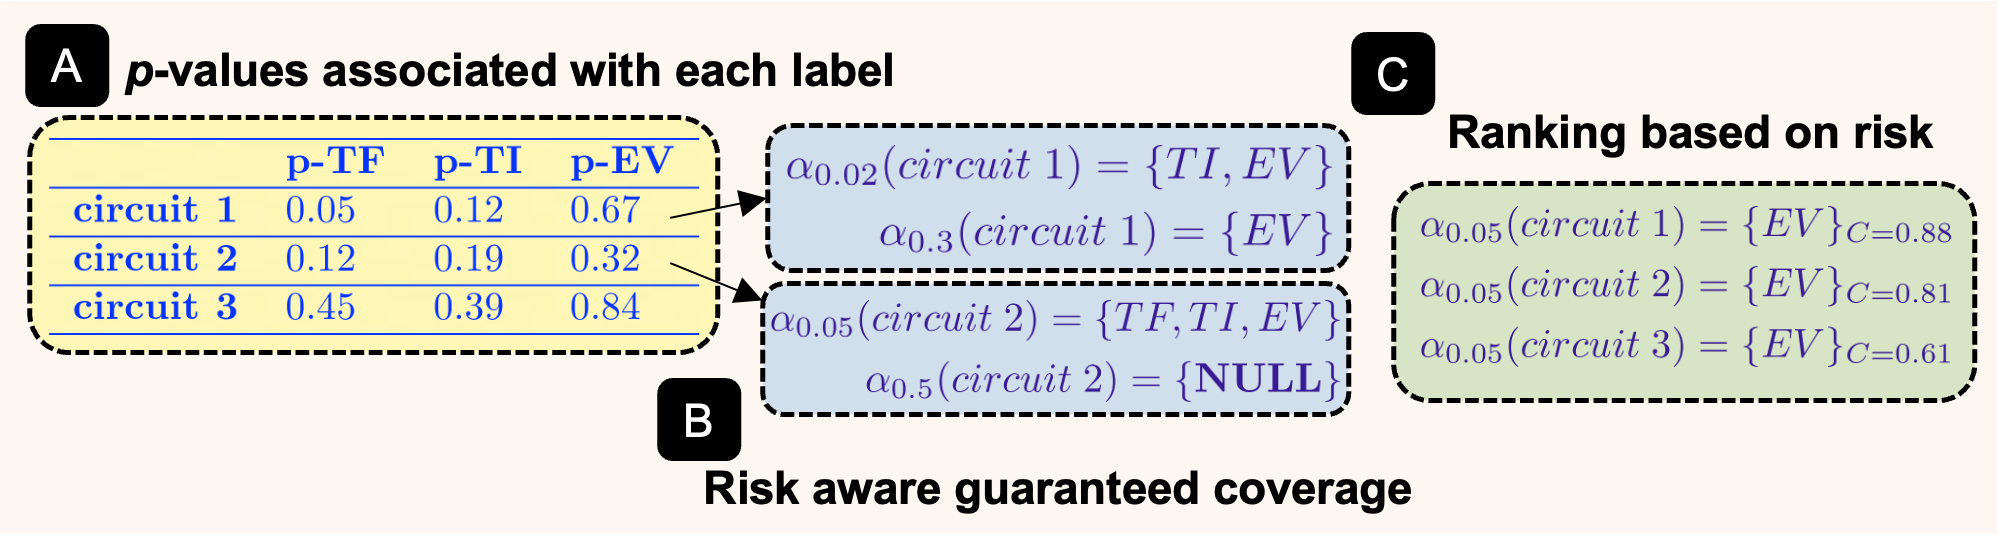
\includegraphics[width=0.5\linewidth]{figs/exp2.png}
  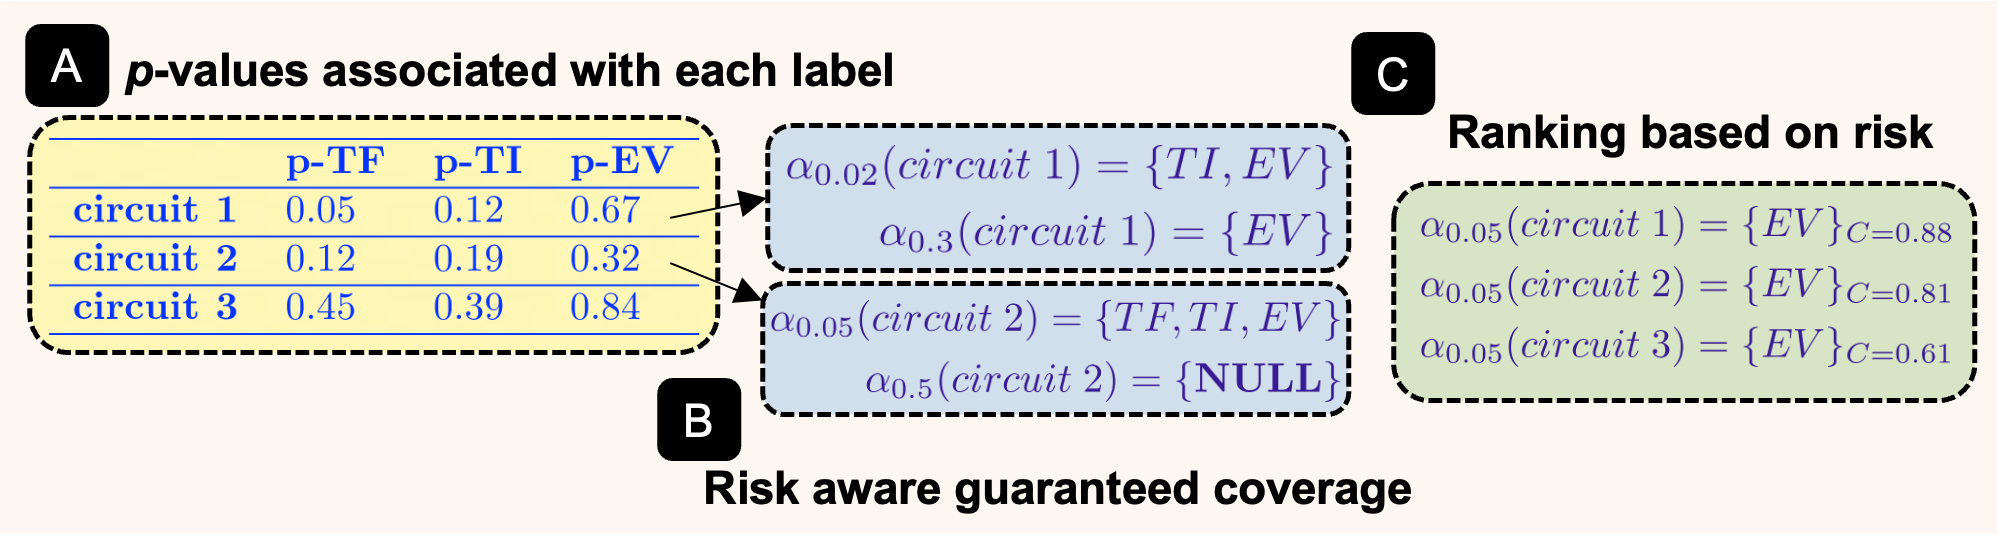
\includegraphics[width=0.5\textwidth]{figs/exp2.png}
  \caption{Interpretation of conformal inference and derived use case for Hardware Trojan detection.}
  \label{fig:inference}
\end{figure*}
\fi

\subsection*{Evolved Dataset}
\label{Sec:EvolvedDataset}
We first generated 10,000 data points using the proposed conformalized GAN  with the given source dataset and picked only 20\% of the evolved dataset. The generated dataset has labels $TF_{G}$ and $TI_{G}$, where as the source dataset has labels $TF_{S}$ and $TI_{S}$. In our evolved dataset, we create three labels as shown below. First, Trojan-Free (TF) which consists of $TF_{S}$ and $TF_{G}$; second, Trojan-Infected (TI) where we only consider the label $TI_{S}$; finally, the third label is Evolved Trojan (T-EV) which consists of the label $TI_{G}$. 
$$Label = \{TF, TI, T-EV \}$$

The dataset is split into training set, calibration set, and test set with ratio 2:1:1. In training dataset we have 1436 TF, 114 TI, and 308 T-EV. For calibration, we have 470 TF, 33 TI, and 117 T-EV. Finally, we have 18\% of T-EV in calibration set and 16\% each in train and test. 



The dataset is split into training set, calibration set, and test set as shown in Table \ref{tab:dataset}. 


\begin{table}[ht]
\centering
\caption{Dataset split for model input}
\begin{tabular}{rrrr}
\hline
\multicolumn{1}{l}{\textit{\textbf{}}} & \textit{Train}   & \textit{Calibration} & \textit{Test}    \\ \hline
\textit{TF}                            & 1436             & 470                  & 471              \\ \hline
\textit{TI}                            & 114              & 33                   & 44               \\ \hline
\textit{T-EV}                          & 308              & 117                  & 105              \\ \hline
Total count                            & 1858    & 620      & 620     \\
\textbf{T-EV}                                   & \textbf{16.50\%} & \textbf{18.87\%}     & \textbf{16.93\%}
\end{tabular}
\label{tab:dataset}
\end{table}



\subsection*{Baseline Model}
\label{Sec:Base}
We can choose any of the classification algorithms as a baseline model because \textbf{PALETTE}, as described in Section \ref{sec:CP}, is algorithm-agnostic. Here, we have used logistic regression as a classifier to detect the evolving HTs, and we evaluate the accuracy of the models as a performance metric. If we use logistic regression to detect HTs, the overall accuracy is 0.85, while if we use conformal inference as a wrapper over the logistic regression, the accuracy increases to 0.88 for $\alpha$ = 0.05 and 0.90 for $\alpha$ = 0.1. This also shows the performance improvement of any classification model when used with underlying conformal inference. A detailed result is shared on our GitHub repository.



\begin{table}[]
\caption{Confusion matrix of base model and conformal inference with significance level of 95\%}
\centering
\begin{tabular}{llllllll}
\hline
              & \multicolumn{3}{l}{\textit{\textbf{Logistic Regression}}} &  & \multicolumn{3}{l}{\textit{\textbf{Conformal Inference}}} \\ \hline
              & \textbf{TF}       & \textbf{TI}      & \textbf{T-EV}      &  & \textbf{TF}       & \textbf{TI}      & \textbf{T-EV}      \\ \hline
\textbf{TF}   & 462               & 8                & 8                  &  & 525               & 24               & 44                 \\ \hline
\textbf{TI}   & 11                & 26               & 2                  &  & 0                 & 10               & 7                  \\ \hline
\textbf{T-EV} & 52                & 0                & 51                 &  & 0                 & 0                & 10                 \\ \hline
\end{tabular}
\label{tab:basecm}
\end{table}



\begin{figure*}[ht]
  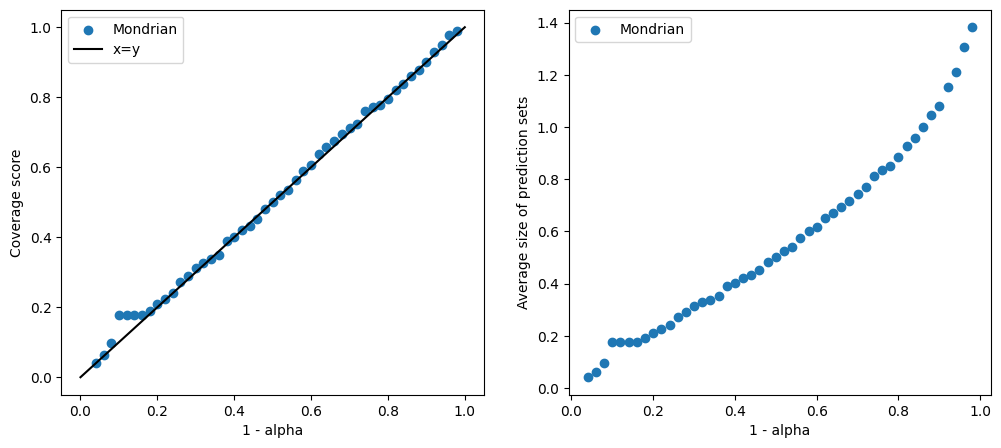
\includegraphics[width=1\linewidth]{figs/cp/cp_score_coverage_and_prediction_Set.png}
  \caption{Effective coverage and average prediction set size for Trust-Hub chip-level Trojan dataset.}
  \label{fig:split}
\end{figure*}

\subsection*{Conformal Inference}
\label{Sec:ConformalInference} 
We will emphasize and reiterate that \textbf{`any'} classification algorithm can be used along with the conformal inference framework, and in our work we have adopted logistic regression with Mondrian conformal predictors. The $p$-value is a measure of confidence in the predictions made by the ML model. It is like a score that tells us how well the model is doing when it makes predictions about new data. To calculate the $p$-value, we compare the model's prediction for a new piece of data with its predictions for the data it was trained on based on hypothesis testing. If the new data is very different from what the model has seen before, the $p$-value will be small, and this can be a sign that the model's prediction for the new data might not be as accurate. So, we need to be careful when interpreting predictions from the model if the $p$-value is too small.

\begin{figure*}[ht]
\centering
  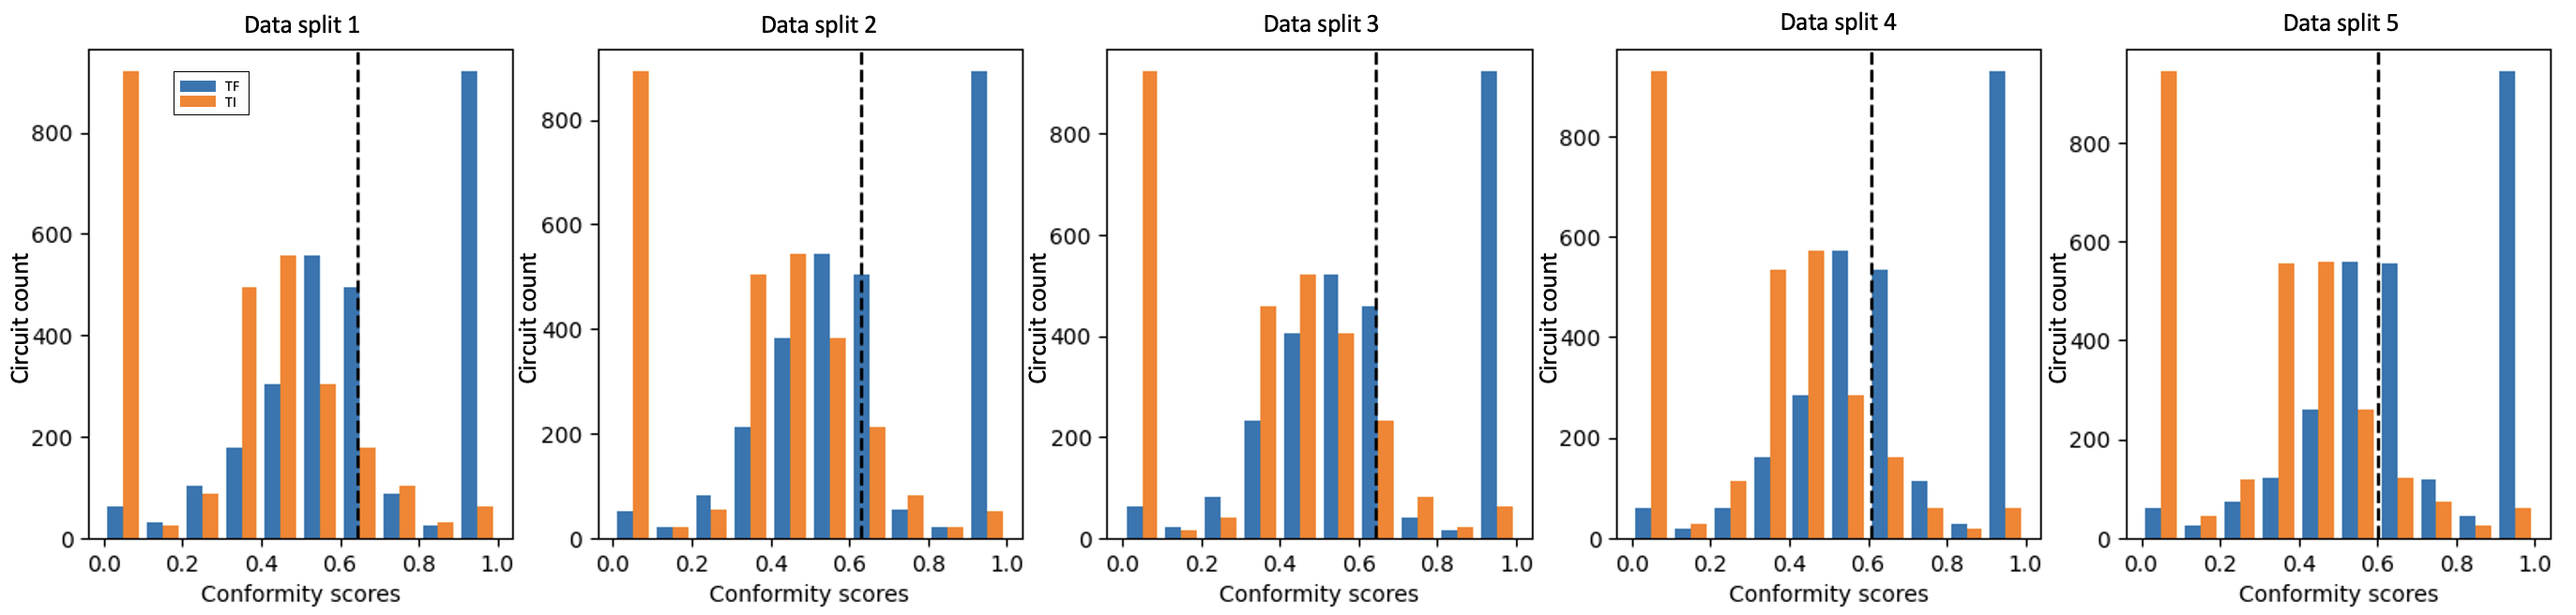
\includegraphics[width=\linewidth]{figs/split.png}
  \caption{Distribution of scores on each five of the calibration fold for the Mondrian conformal predictor for GAINESIS dataset.}
  \label{fig:b_fold}
\end{figure*}

\begin{table}[t]
\centering
\caption{Conformal inference and associated p-vales for Trust-Hub chip-level Trojan dataset.}
\begin{tabular}{lcccrrrrr}
\hline
  & \textbf{TF} & \textbf{TI} & \textbf{T-EV} & \textbf{pTF} & \textbf{pTI} & \textbf{pT-EV} & \textbf{y\_pred} & \textbf{Conf}\\ \hline
1 & T           & F           & F           & 0.319        & 0            & 0.003        & TF  & 0.997             \\ \hline
2 & T           & F           & F           & 0.243        & 0.002        & 0.006        & TF  & 0.994             \\ \hline
3 & T           & T           & F           & 0.161        & 0.078        & 0.016        & TF   & 0.992            \\ \hline
4 & T           & T           & T           & 0.114        & 0.053        & 0.119        & T-EV  & 0.886           \\ \hline
5 & T           & F           & F           & 0.645        & 0.001        & 0.004            & TF   & 0.996           \\ \hline
6 & F           & F           & T           & 0.653            & 0            & 0.971        & T-EV    & 0.365         \\ \hline
7 & T           & F           & F           & 0.3          & 0            & 0.002        & TF      & 0.998         \\ \hline
\end{tabular}
\label{tab:conformalresults}
\end{table}

\begin{table}[t]
\centering
\caption{Conformal inference for GAINESIS dataset.}
\begin{tabular}{lllll}
\hline
\textbf{circuit}        & \textbf{TI}             & \textbf{TF}             & \textbf{y-pred} & \textbf{Conf}           \\ \hline
1                       & FALSE                   & TRUE                    & TF              & 0.891                   \\ \hline
2                       & FALSE                   & TRUE                    & TF              & 0.796                   \\ \hline
3                       & FALSE                   & TRUE                    & TF              & 0.996                   \\ \hline
4                       & FALSE                   & TRUE                    & TF              & 0.997                   \\ \hline
\multicolumn{1}{c}{...} & \multicolumn{1}{c}{...} & \multicolumn{1}{c}{...} & ...             & \multicolumn{1}{c}{...} \\ \hline
4596                    & FALSE                   & TRUE                    & TF              & 1                       \\ \hline
4597                    & FALSE                   & TRUE                    & TF              & 0.991                   \\ \hline
4598                    & TRUE                    & FALSE                   & TI              & 0.995                   \\ \hline
4599                    & FALSE                   & TRUE                    & TF              & 0.989                   \\ \hline
4600                    & FALSE                   & TRUE                    & TF              & 0.992                   \\ \hline
\end{tabular}
\label{tab:binary_cp}
\end{table}

The results obtained after implementing conformal inference for detecting evolving HTs are shown in Table \ref{tab:conformalresults}. Each row represents the circuit and the truth value in columns TF, TI, and T-EV. In addition, the $p$-values for each label are mentioned in the columns pTF, pTI, and pT-EV. Finally, the detected Trojan is mentioned in column y\_pred with $\alpha$ = 0.05. The column \textit{Conf} represents the confidence score of each detected label for each circuit, which is obtained by $1 - 2^{nd}p_{max}$. An application of conformal inference is the improvement of detection quality for evolving HTs. For example, in Table \ref{tab:conformalresults}, circuit 2 is detected as Trojan-Free because the $p$-values of TI and T-EV are less than the value of $\alpha$ = 0.05. The circuit 4 and 6 are detected as infected with an evolved Trojan. In circuit 4, we see that $p$-values for TF, TI, and T-EV are greater than the value of $\alpha$, so all the labels are set as T (True), and the maximum of the $p$-value is specified for the detected label. For example, with conformal inference, we can say that with 95\% detection guarantee (as $\alpha$ = 0.05 decided by the user), circuit 4 is detected as an evolving Trojan with a confidence score of 0.886. This helps the end user have granular-level reasoning for trustworthy and robust decision-making.

We also share the results for binary labels (TF, TI) on the GAINESIS dataset in Table \ref{tab:binary_cp}. The method was validated on $4600$ synthetic circuits with and without Trojans, and the corresponding confidence score is shown in the column \textit{Conf}.

\begin{table}[t]
\centering
\caption{Comparison of conformal predictors with corresponding significance level on Trust-Hub chip-level Trojan dataset.}
\begin{tabular}{ccccc}
\hline
\textbf{alpha} & \textbf{mondrian} & \textbf{raps} & \textbf{naïve} & \textbf{top\_k} \\ \hline
0.05           & 10                & 37            & 35             & 0               \\ \hline
0.5            & 45                & 57            & 57             & 61              \\ \hline
0.9            & 45                & 61            & 61             & 61              \\ \hline
\end{tabular}
\label{tab:racp}
\end{table}

Furthermore, we also explored variations of conformal predictors as described in \cite{bates2021distribution}. Table \ref{tab:racp} shows that the Mondrian conformal predictor is very strict on detecting the evolved hardware Trojans as compared to the risk-adaptive prediction set \textit{raps}, \textit{naive}, and \textit{top\_k} methods with varying significance levels. The \textit{naive} and \textit{top\_k} first get the model output of the true class, and \textit{naive} makes the estimated set prediction by getting quantiles from the score distribution, while \textit{top\_k} gets the quantiles from the distribution of the ordered positions of the true label. The \textit{raps} method first sorts the model output in decreasing order to get cumulative output of the true class and then uses it to obtain quantiles from cumulative score distributions. Furthermore, with a very high coverage of 95\% ($\alpha$ = 0.05), \textit{raps} and \textit{naive} detect almost three times more Trojans as compared to Mondrian, while the detection coverage becomes almost similar when the coverage level is increased.

%%%%%%%%%%%%%%%%%%%%%%%%%%%%%%%%%%%%%%%%%%%%%%%%%%%%%
    % Performance metrics 
%%%%%%%%%%%%%%%%%%%%%%%%%%%%%%%%%%%%%%%%%%%%%%%%%%%%%

\subsection*{Performance Metrics}
\label{Sec:Performance}
Unlike classification task which produces Receiver Operating Characteristic (ROC) and Area Under Curve (AUC), conformal inference produces \textit{effective coverage} and \textit{efficiency}, i.e., average prediction set size, as performance metrics. The limitation of ROC and AUC is that they can be impacted by an imbalanced dataset. In Fig. \ref{fig:split} we show the two different performance metrics for Mondrian conformal predictors. The coverage score measures the proportion of instances in which the true label falls within the predicted region. It is typically measured at different confidence levels. Higher coverage indicates a more conservative prediction method. Now, since validity is guaranteed for all conformal predictors, the key performance metric is efficiency, i.e., the size of the label sets, where smaller sets are more informative and indicate higher efficiency. It is also a direct measure of how good the conformal predictor is at rejecting class labels.

When evaluating conformal prediction methods, there are several metrics that can be used to assess their performance. In Table \ref{tab:performance} we show the various performance metrics associated with the detection mechanism for significance levels ranging from 0.05 to 0.9. For example, avg\_c indicates the average number of class labels in the prediction sets; this metrics serves as a straightforward indicator of the conformal predictor's ability to accurately discard class labels.

%A derived metric, \textit{Efficiency-Validity Trade-off} is not shown the table, but it shows the balance between the efficiency and validity of the conformal prediction method and help determine the optimal trade-off point that provides a good balance between efficiency and validity. 

The significance level is like a threshold that controls how often the ML model makes incorrect predictions. If we set a higher significance level, the model will make fewer errors, but its predictions may be less precise. So, we need to find the right balance to get the best results from our model.

Furthermore, we also show the performance metrics for the GAINESIS dataset in Fig. \ref{fig:b_fold}. We examine the conforming score (expected label) distribution on each of the five calibration folds for the Mondrian conformal predictor and observe that there is no major difference in the conforming score for each calibration split.

\begin{table}[t]
\centering
\caption{Performance metrics of conformal inference on Trust-Hub chip-level Trojan dataset.}
\begin{tabular}{lllll}
\hline
\textbf{sig} & \textbf{mean\_err} & \textbf{avg\_c} & \textbf{n\_correct} & \textbf{mean\_T-EV} \\ \hline
0.05         & 0.049                 & 1.040           & 589                 & 0.012               \\ \hline
0.1          & 0.102                 & 0.941           & 556               & 0.045               \\ \hline
0.2          & 0.204                 & 0.812           & 493             & 0.133               \\ \hline
0.3          & 0.303                 & 0.701           & 431             & 0.220               \\ \hline
0.4          & 0.406                 & 0.596           & 367            & 0.319               \\ \hline
0.5          & 0.504                 & 0.497           & 307           & 0.423               \\ \hline
0.6          & 0.604                 & 0.397           & 245             & 0.536               \\ \hline
0.7          & 0.702                 & 0.298           & 184            & 0.650               \\ \hline
0.8          & 0.798                 & 0.202           & 125           & 0.764               \\ \hline
0.9          & 0.900                 & 0.100           & 61         & 0.884               \\ \hline
\end{tabular}
\label{tab:performance}
\end{table}

\begin{figure*}[h]
\centering
  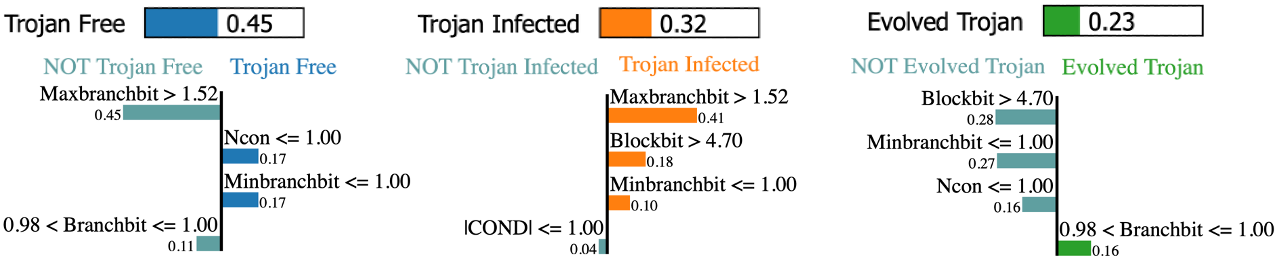
\includegraphics[width=\linewidth]{figs/lime.png}
  \caption{Calibrated explanation for rejecting a decision.}
  \label{fig:lime}
\end{figure*}

%%%%%%%%%%%%%%%%%%%%%%%%%%%%%%%%%%%%%%%%%%%%%%%%%%%%%
    % Ranking of prediciton based on confidence 
%%%%%%%%%%%%%%%%%%%%%%%%%%%%%%%%%%%%%%%%%%%%%%%%%%%%%
\subsection*{Risk-Aware Ranking}
\label{Sec:Risk}
We leverage \textit{confidence score} from the conformal inference as a ranking mechanism for evolved HTs. For the below given circuits 12, 13, and 14 from the Trust-Hub dataset, we calculated their confidence score (C) with $\alpha$ = 0.05. 
$$
\begin{aligned}
& \alpha_{0.05}(\text { circuit } 12)=\{T-E V\}_{C=0.88} \\
& \alpha_{0.05}(\text { circuit } 13)=\{T-E V\}_{C=0.81} \\
& \alpha_{0.05}(\text { circuit } 14)=\{T-E V\}_{C=0.61}
\end{aligned}
$$
Confidence in a model's prediction is determined by its $p$-value which indicates the probability of obtaining a similar outcome under the \textit{NULL} hypothesis. Higher confidence implies greater accuracy. This metric is defined as:
$$\text{Confidence} (x) = \sup \{1 - \epsilon : |\Gamma_\epsilon (x)| \leq 1\} $$

By ranking the predictions, conformal prediction can offer a more informative way to assess the reliability of individual predictions. The ranked list allows decision-makers to set thresholds or confidence levels for accepting or rejecting predictions based on their position in the ranking.

This provides a flexible tool for controlling the trade-off between accuracy and reliability in different applications. In Table \ref{tab:confcred} we show the \textit{confidence} and \textit{credibility} of the detected labels. The credibility is obtained by considering the maximum $p$-value of the given set prediction. Credibility quantifies the quality of the new data points. 

\begin{table}[t]
\centering
\caption{Adoption of confidence for risk-aware ranking on Trust-Hub chip-level Trojan dataset.}
\begin{tabular}{llll}
\hline
  & \textbf{confidence} & \textbf{credibility} & \textbf{y\_pred} \\ \hline
1 & 0.997               & 0.319                & TF               \\ \hline
2 & 0.994               & 0.242                & TF               \\ \hline
3 & 0.922               & 0.162                & TF               \\ \hline
4 & 0.886               & 0.119                & T-EV             \\ \hline
5 & 1                   & 0.645                & TF               \\ \hline
6 & 0.999               & 0.97                 & T-EV             \\ \hline
7 & 0.998               & 0.301                & TF               \\ \hline
\end{tabular}
\label{tab:confcred}
\end{table}


%%%%%%%%%%%%%%%%%%%%%%%%%%%%%%%%%%%%%%%%%%%%%%%%%%%%%
    %Explainability 
%%%%%%%%%%%%%%%%%%%%%%%%%%%%%%%%%%%%%%%%%%%%%%%%%%%%%

\subsection*{Calibrated Explanations for Reject}
\label{Sec:explain}
When the model is not able to detect evolving HT, the model simply says, \textit{``I don't know''} by giving a \textit{NULL} set as the output. In a risk-sensitive domain, a model with no output is better than a decision that is not confident. Our framework also provides the reason for rejecting the decision with a calibrated explanation, as shown in Fig. \ref{fig:lime}, which is different from traditional explainable methods. If we apply a significance level of 0.5 to the given circuit, none of the $p$-values for TF (0.45), TI (0.32), and T-EV (0.23) exceed the significance level. As a result, we reject the decision. The explanation for this rejection is based on Local Interpretable Model-agnostic Explanations (LIME) \cite{dieber2020model}. However, the differentiating factor as compared to SHAP (which disregards causality and is affected by human bias) is that before providing any explanation for the rejection, we ensure that it is calibrated. The approach begins by creating modified versions of the original instance called perturbed instances, where small random changes are introduced. Conformal prediction is then utilized to create prediction regions that estimate the reliability or confidence level of the explanations, and LIME is then used again on these perturbed instances to generate explanations for each of them. The prediction regions obtained through conformal prediction act as a calibration mechanism, guaranteeing that the explanations accurately reflect their level of reliability. 

%Calibration of the underlying model to ensure that probability estimates are closer to reality.

\iffalse 
\begin{table}[ht]
\centering
\caption{Rejecting a decision based on the significance level on Trust-Hub chip-level Trojan dataset}
\begin{tabular}{llll}
\hline & \text { p-TF } & \text { p-TI } & \text { p-EV } \\
\hline \text { circuit 23 } & 0.05 & 0.12 & 0.67 \\
\hline \text { circuit 24 } & 0.12 & 0.19 & 0.32 \\
\hline \text { circuit 25 } & 0.45 & 0.39 & 0.84 \\
\hline
\end{tabular}
\label{tab:reject}
\end{table}
\fi 

%%%%%%%%%%%%%%%%%%%%%%%%%%%%%%%%%%%%%%%%%%%%%%%%%%%%%
    %Discussion and Conclusion
%%%%%%%%%%%%%%%%%%%%%%%%%%%%%%%%%%%%%%%%%%%%%%%%%%%%%
\section*{Discussion}


We introduced a method for creating evolving dataset using a conformalized generative adversarial network. Afterward, we introduced \textbf{PALETTE}, a framework capable of detecting evolving hardware Trojans without being tied to a specific algorithm. We also implemented a unique method to reject decisions by offering a well-explained rationale. Notably, \textbf{PALETTE} proved effective in detecting hardware Trojans, providing an assigned uncertainty level for each detection.

Our results highlighted opportunities for fellow researchers in hardware security, especially those in logic locking. We encourage them to reconsider how machine learning solutions are applied and redefine the metrics for evaluating their methods. While acknowledging there's no one-size-fits-all solution for zero-day attacks, we emphasize the importance of robust methods to minimize the risk of attacks. A proactive defense approach, exemplified by our proposed method, plays a crucial role in strengthening systems against potential threats.

\endgroup
\newpage

\phantomsection
\addcontentsline{toc}{section}{3. MULTIMODAL LEARNING FOR HARDWARE TROJAN DETECTION}
\section*{Chapter 3 \\ MULTIMODAL LEARNING FOR HARDWARE TROJAN DETECTION}
\begingroup
\RaggedRight

\begin{quote}
"On what is fear: non-acceptance of uncertainty. If we accept that uncertainty it becomes an adventure!"
\newline
\hfill  — \textit{Jalāl al-Dīn Muḥammad Rūmī}
\end{quote}

\section*{Introduction}
Hardware Trojan (HT) insertion has become a major concern in today's fabless semiconductor manufacturing since attackers can make malicious modifications for a variety of reasons, such as information leakage, incorrect operation, or inflicting damage on the chip \cite{salmani2017hardware,  Regazzoni:HTDetection, Guin:HTDetection, Salmani:HTDetection}. The possibility of HTs being inserted at different manufacturing stages increases, presenting a significant security threat to hardware systems. Vulnerabilities range from RTL code and third-party IP integration in the design phase to potential insertions during EDA processes like synthesis, optimization, and place-and-route. Mask preparation \cite{belous2020methods} and lithography in wafer fabrication offer additional points of vulnerability. Packaging and testing phases also present opportunities for Trojan inclusion, as do third-party manufacturing and distribution in post-production. Robust security measures \cite{narasimhan2011tesr}, including hardware design practices \cite{muralidhar2021contrastive}, supply chain management \cite{chang2023supplier, panduro2023effective}, and thorough post-manufacturing testing \cite{monjur2023hardware}, are imperative to mitigate these risks in the semiconductor industry.
To effectively address the challenges posed by HTs in the current technological landscape, a comprehensive approach is imperative. This includes design integrity verification through formal verification \cite{nahiyan2017hardware} and simulation-based testing, coupled with the deployment of advanced Intrusion Detection Systems (IDS) for continuous monitoring and timely detection of suspicious behavior. Hardware security measures like obfuscation \cite{nishita2023hardware}, encryption \cite{chandra2023efficient}, and secure boot \cite{monjur2023hardware} should be integrated to fortify against HT insertion and minimize their impact if detected. Secure boot processes \cite{monjur2023hardware} and real-time monitoring further fortify chip integrity, while adherence to recognized security certification standards ensures compliance with industry best practices. 
While comprehensive approaches are vital for countering HTs, they entail certain drawbacks. Formal methods and simulation-based testing can be resource-intensive and time-consuming. Intrusion detection systems may yield false alarms, disrupting operations. %Hardware security measures may introduce performance overhead and complexity. 
Establishing a secure supply chain can limit flexibility in supplier selection. Post-manufacturing testing adds time and cost. 
Thus, striking a balance between these considerations and the need for robust Trojan defenses is crucial for semiconductor manufacturers.

Recently, Machine Learning (ML) has emerged as a powerful tool for detecting HTs \cite{gubbi2023hardware, huang2020survey, liakos2019machine, koblah2023survey, koylu2023survey}. %in fabless semiconductor manufacturing. 
It leverages algorithms to identify intricate patterns indicative of Trojans, even in increasingly sophisticated attacks. By training on diverse datasets, ML models can classify circuits as Trojan-free or Trojan-infected. Real-time processing enables continuous monitoring and immediate threat response. However, challenges exist, for example, acquiring large and diverse datasets, especially for rare Trojans, which can be difficult. Moreover, models are susceptible to adversarial attacks \cite{west2023towards}, potentially undermining their decision-making. Interpretability \cite{li2022interpretable} and explainability \cite{caruana2020intelligible} are crucial for trust but can be complex in this context. Additionally, resource-intensive training and deployment may limit accessibility for smaller manufacturers. Continuous retraining is necessary to adapt to evolving Trojan techniques \cite{Vishwakarma:ICCAD}, adding complexity to maintenance. 

Our goal in this paper is to address the gaps in the current ML-based approaches for identification of HTs by %leveraging two modalities of the circuit representation for an improved accuracy. In this paper, we propose 
proposing \textbf{NOODLE}, an u\textbf{N}certainty-aware hardware Tr\textbf{O}jan detecti\textbf{O}n using multimo\textbf{D}al deep \textbf{LE}arning. The proposed method uses graph representation and tabular data and performs binary classification.

\subsection*{Related Works}
The emphasis in traditional ML approaches for HT detection has primarily been on modeling techniques. This entails the development and implementation of algorithms aimed at enhancing the overall accuracy of HT detection. The model takes as input features extracted from the Register Transfer Level (RTL) code, which are represented both in tabular and graphical forms depicting the circuit. Various surveys on the application of ML in detecting HT attacks have been conducted.  
Many research papers have concentrated on extracting features from Register Transfer Level (RTL) or gate-level netlists and employing ML models such as Support Vector Machine (SVM) \cite{bao2014application}, Neural Network (NN) \cite{hasegawa2017hardware}, eXtreme Gradient Boosting (XGB) \cite{dong2019machine}, and the Random Forest (RF) classifier \cite{hasegawa2017trojan}. In \cite{ashok2022hardware}, image classification techniques are also employed. %while in \cite{10027082}, a multimodal image processing approach is utilized, the only paper that detects HTs using multimodal image processing.

Multimodal Deep Learning (DL) has been a well-explored topic in the Artificial Intelligence (AI) community. Early research, exemplified by Deep Boltzmann Machines (DBM) focused on the model's capacity to understand probability distributions across inputs with multiple modes \cite{srivastava2012multimodal}. Additionally, applications of uncertainty-aware multimodal learning \cite{wang2022uncertaintyaware} have been successfully demonstrated in healthcare \cite{sarawgi2021uncertainty} and in scenarios involving multimodal task distributions \cite{almecija2022uncertaintyaware}, particularly in safety-critical environments. In our work, we target the fusion of graph \cite{ektefaie2023multimodal, kim2023heterogeneous} and Euclidean data as the modalities of interest along with uncertainty estimation. 

Moreover, when working in the hardware security domain, it is expected to have fewer data points that are malicious or Trojan-infected. In this context, it is necessary to work with small data \cite{nyiri2023can} and this has been achieved in various domains such as material science \cite{xu2023small} and anomaly detection \cite{ghamisi2023anomaly}.

\subsection*{Contributions}
In this paper, we investigate the feasibility of applying a multimodal ML approach for HT identification by deriving two data representations of circuits. The first is graphical representation \cite{yu2021hw2vec} of circuits, and the second is euclidean data \cite{px6s-sm21-22} derived by processing the Abstract Syntax Tree (AST) of the RTL files (Verilog). Although the use of multimodal approaches for improved model accuracy has been used in other domains, we do not see any application in Trojan identification. For uncertainty-aware multimodal learning, we believe the logic should be implemented at the information fusion level of the modalities, and thus, we leverage the $p$-values aggregation with conformal prediction. Our main contributions are as follows:
\begin{itemize}
    \item Proposing a multimodal learning approach using graph and euclidean data of the hardware circuits. To the best of our knowledge, this study is the first to investigate and implement a multimodal approach for HT detection.
    \item Suggesting a model fusion approach using $p$-values with an uncertainty quantifier. By employing $p$-values as statistical measures, we can systematically assess each modality's contribution to the overall prediction. This not only enhances the interpretability of the fusion process but also enables more robust decision-making.
    \item Addressing the challenges of missing modalities and solving the issue of handling an imbalanced and small dataset by leveraging generative adversarial networks.
\end{itemize}

\begin{figure*}[ht]
  \centering
   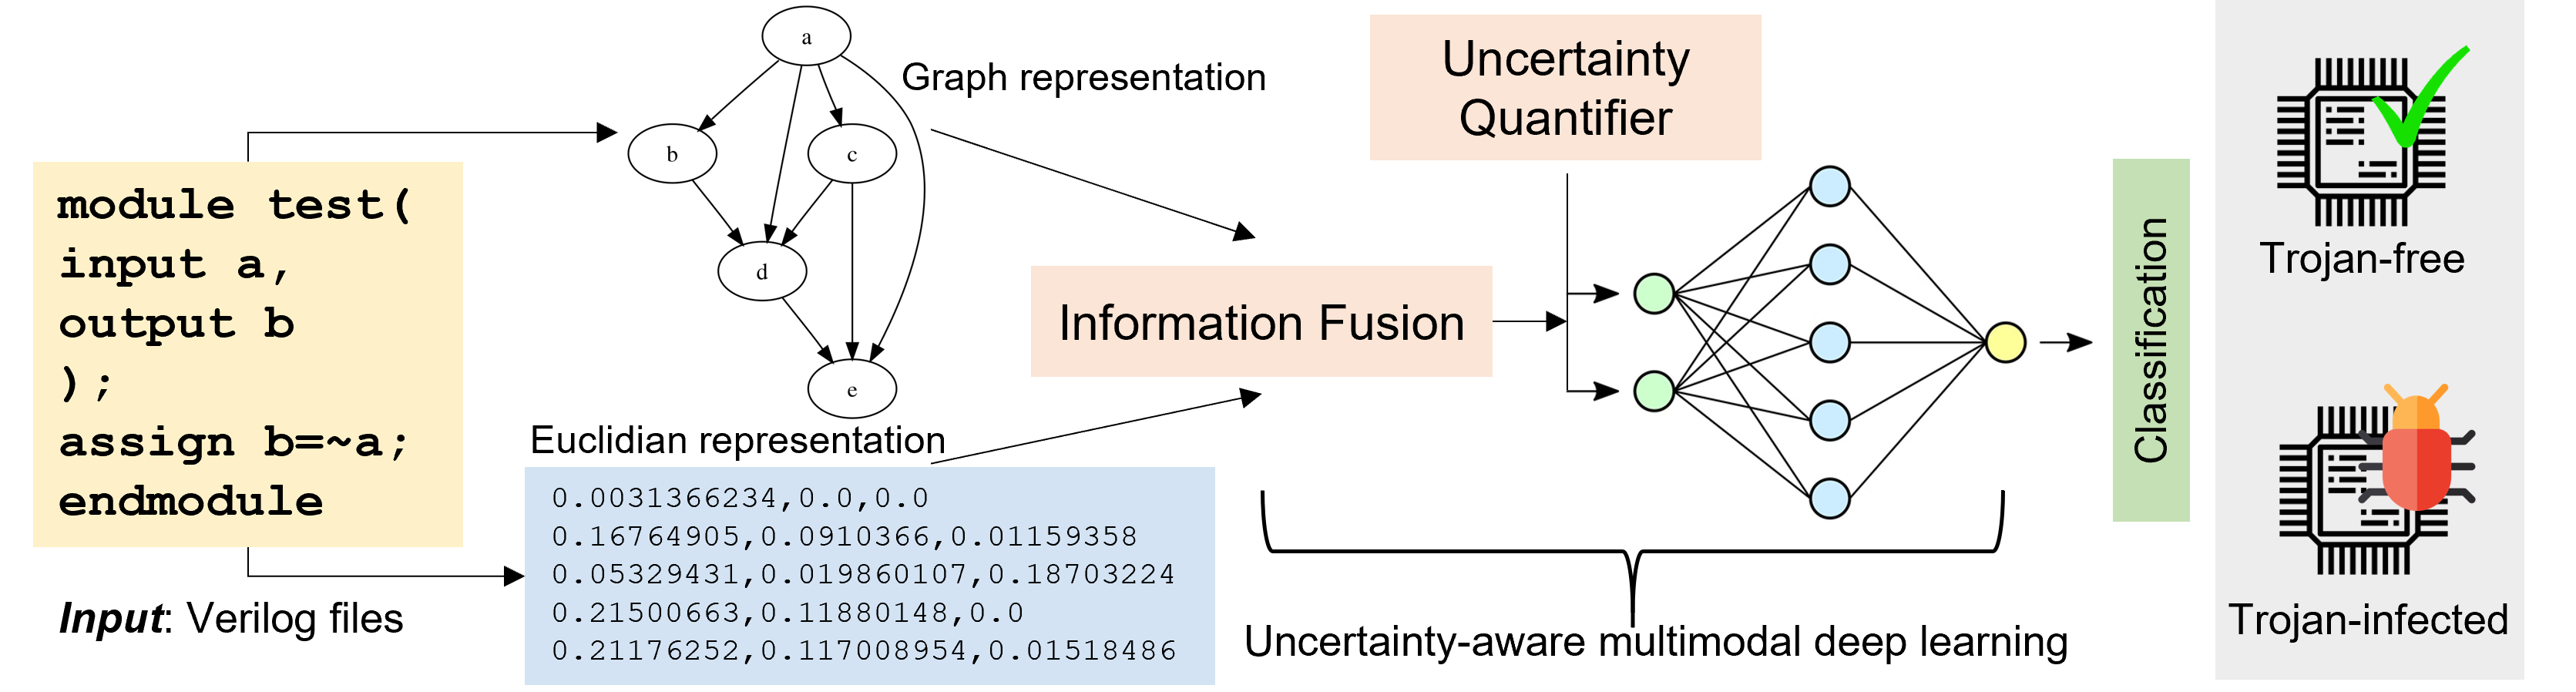
\includegraphics[width=1\textwidth]{figs/BigPicture.png}
   \caption{NOODLE framework: The input consists of an RTL file (Verilog), which undergoes conversion into both graph and Euclidean representations, and then input into a multimodal deep learning classifier. This classifier yields a decision indicating whether the circuit is Trojan-infected or Trojan-free.}
  \label{fig:intro}
\end{figure*}

\section*{Preliminaries}
\label{Sec:Prelem}
%Background 

%%%%%%%%%%%%%%%%%%%%%%%%%%%%%%%%%%%%%%%%%%%%%%%%%%%%%
    %Multimodal learning 
%%%%%%%%%%%%%%%%%%%%%%%%%%%%%%%%%%%%%%%%%%%%%%%%%%%%%
\subsection*{Multimodal Learning}
\label{sec:multimodal}
Multimodal learning \cite{ngiam2011multimodal} addresses complex problems by integrating information %from different data modals. It combines insights 
from multiple modalities, such as text, images, and audio, to obtain a comprehensive understanding of a given phenomenon. In our case, we use graphical data and tabular representations of the source circuits. This approach enables models to capture nuanced relationships that may be overlooked when considering each modality in isolation, and thus empowers the model to make more robust predictions.

From a mathematical perspective, multimodal learning involves the integration of data representations into a unified framework. Let \(X_1, X_2, ..., X_M\) represent \(M\) different modalities of data, each with their respective feature spaces \(\mathcal{F}_1, \mathcal{F}_2, ..., \mathcal{F}_M\). The task is to learn a mapping \(f\) that captures the relationships between these modalities. Mathematically, this can be formulated as:
\begin{equation}
f: \mathcal{F}_1 \times \mathcal{F}_2 \times ... \times \mathcal{F}_M \rightarrow \mathcal{Y}
\end{equation}
where \(\mathcal{Y}\) is the target space, representing the desired prediction.

The challenge lies in effectively combining information from diverse modalities, which can be approached through various techniques such as late fusion or early fusion. %, and cross-modal attention mechanisms. 

In late fusion \cite{trong2020late}, features are extracted independently from each modality and then combined at a later stage. This approach treats modalities as separate entities until a decision needs to be made and can be represented as:
\begin{equation}
f(x_1, x_2, ..., x_M) = g(h_1(x_1), h_2(x_2), ..., h_M(x_M))
\end{equation}
where \(h_i\) represents feature extraction for modality \(i\), and \(g\) combines the extracted features.

In early fusion \cite{nguyen2021gefa}, information from different modalities is combined at the input level, resulting in a joint feature representation which can be expressed as:
\begin{equation}
f(x_1, x_2, ..., x_M) = h(x_1, x_2, ..., x_M)
\end{equation}
where \(h\) combines the raw input data from all modalities.

%Cross-modal attention mechanisms \cite{wang2021cross} dynamically allocate attention weights to different modalities based on the context of the input. This allows the model to focus on relevant information for a given task, enhancing its adaptability and performance.

%%%%%%%%%%%%%%%%%%%%%%%%%%%%%%%%%%%%%%%%%%%%%%%%%%%%%
    %Calibration
%%%%%%%%%%%%%%%%%%%%%%%%%%%%%%%%%%%%%%%%%%%%%%%%%%%%%
\subsection*{Calibrated Prediction}
\label{sec:Calibration}
Calibration involves ensuring that a model's confidence score accurately reflects the true probability of the prediction's correctness \cite{ovadia2019can}. Let $X$ be the input data, and $Y$ be the output label. Given a training dataset $D = {(x_1, y_1), (x_2, y_2),..., (x_n, y_n)}$, the goal is to learn a function $f$ that can predict the correct output label $y$ for a given input $x$. The output of the model for an input $x$ can be denoted as $f(x)$, and the true probability of the prediction's correctness can be denoted as $P(y=1|x)$. A calibrated model produces a confidence score $g(x)$ that reflects the true probability of correctness of the prediction. The goal of calibration is to ensure that the confidence score $g(x)$ is well-calibrated, i.e., $P(y=1|g(x)=p) = p$ for all $p$ in the range $[0, 1]$.

Calibration is a crucial aspect in HT detection since it aids in determining the likelihood of the existence of a Trojan in a circuit, which can have a significant impact on decision-making. In situations where a model's confidence score is high, but the likelihood of a Trojan's presence is low, it is reasonable to assume that the circuit does not contain a Trojan. Conversely, if the confidence score is low but the likelihood of a Trojan's presence is high, further investigation of the circuit is necessary.

\begin{algorithm}[!b]
\small
\SetKwInOut{Input}{Input}
\SetKwInOut{Output}{Output}
\Input {Number of data sources $N$; \newline
Training sets for each data source $T_1 = \{(x^{(1)}_1, y_1), \ldots, (x^{(1)}_n, y_n)\}, \ldots, T_N = \{(x^{(N)}_1, y_1), \ldots, (x^{(N)}_n, y_n)\}$, where $x^{(j)}_i$ is the $i$th data point belonging to the $j$th data source and $y_i$ is the class label of the $i$th data point; \newline
Number of classes $M$; \newline
Class labels $y^{(i)} \in Y = \{y^{(1)}, y^{(2)}, \ldots, y^{(M)}\}$; \newline
Classifiers $S_1, \ldots, S_N$ for each data source; \newline
Confidence level $E$.}

\Output {Conformal prediction regions $r_E = \{y^{(j)} : \hat{p}_j > 1 - E, y^{(j)} \in Y\}$.}

Get the new unlabeled example w.r.t each data source $x^{(1)}_{n+1}, \ldots, x^{(N)}_{n+1}$.

Evaluate conformal predictors and classifiers $S_1, \ldots, S_N$ corresponding to each data source, compute $p$-values $p^{(i)}_j$, where $i = 1, \ldots, N$ corresponds to the $i$th data source and $j = 1, \ldots, M$ corresponds to the $j$th class label.

\For {each class label $y^{(j)}$, $j = 1, \ldots, M$}{
    Compute $p$-value, $\hat{p}_j$, of combined hypothesis from $N$ modalities}

\Return $r_E$.
\caption{Uncertainty-aware information fusion}
\label{algo:mcp}
\end{algorithm}

%%%%%%%%%%%%%%%%%%%%%%%%%%%%%%%%%%%%%%%%%%%%%%%%%%%%%
    %Conformal Prediction
%%%%%%%%%%%%%%%%%%%%%%%%%%%%%%%%%%%%%%%%%%%%%%%%%%%%%
\subsection*{Conformal Prediction}
\label{sec:CP}
Conformal Prediction (CP) is a ML framework that assesses prediction uncertainty by generating sets of possible predictions \cite{shafer2008tutorial}. This approach strengthens the inference of conventional models, ensuring their reliability and enabling confidence estimation for individual predictions. It is worth noting that minority classes often bear a disproportionate burden of errors when label-conditional validity is lacking \cite{lofstrom2015bias}. Nevertheless, this challenge can be mitigated by ensuring label-conditional validity, which guarantees that the error rate, even for the minority class, will eventually converge to the selected significance level in the long run. 

In certain instances, CP may yield uncertain predictions, signifying that prediction sets contain more than one possible value. This happens when none of the labels can be rejected at the specified significance level. Moreover, when employing CP, the confusion matrix differs from the conventional one due to the distinctive nature of prediction sets, which encompass multiple values rather than a single one. In binary classification scenarios, it is crucial to consider the number of accurately predicted instances, where the prediction set contains only the correct label, as well as the number of inaccurately predicted instances, where the prediction set contains only the incorrect label. Additionally, it is important to account for the number of inconclusive predictions, which occur when the prediction set contains both labels, along with the number of instances with an empty prediction set. Moreover, in cases where providing a single-point prediction may be more appropriate than a prediction set or interval in a hedged forecast, opting for the label with the highest $p$-value is a straightforward and reasonable choice. This point prediction can be hedged by incorporating additional information that characterizes the uncertainty.

There has been limited exploration of the application of CP in modal fusion \cite{balasubramanian2015conformal}. This method entails treating individual data sources as separate hypothesis tests within the CP framework. Subsequently, it utilizes $p$-value combination techniques as a test statistic for the combined hypothesis after the fusion process. Our approach relies on the Mondrian Inductive Conformal Prediction (ICP) methodology \cite{bostrom2021mondrian} outlined in Algorithm \ref{algo:mcp} for the uncertainty-aware fusion of various modalities during classification. This algorithm can be effectively extended for both early and late fusion of the modalities.

In the domain of HT detection, it is not only important to have a high level of confidence in the predictions made by a model but also a guarantee of the coverage of each prediction. The property of guaranteed coverage is an inherent property of CP, which provides statistical guarantees of the correctness of the model's predictions \cite{angelopoulos2023conformal}. The theoretical guarantee of coverage is based on the significance level, which is the probability of the model making a mistake. For example, if we set the significance level to $0.05$, it means that we allow the model to make mistakes $5\%$ of the time.
 
The theoretical guarantee of coverage is valid for any input $x$, that the true output label $y$ will be contained in the prediction set $C(x)$ with a probability of at least $1 - \alpha$, where $\alpha$ is the significance level. Mathematically, this can be expressed as:
\begin{equation}
P(y \in C(x)) \geq 1 - \alpha
\end{equation}

In other words, the probability of making a mistake is bounded by $\alpha$, and as $\alpha$ decreases, the size of the prediction set decreases, leading to higher confidence in the model's predictions. For example, if we set $\alpha = 0.05$, it means that we are $95\%$ confident that the true output label $y$ is contained in the prediction set $C(x)$ for any input $x$.

%\section{Design Principles}
%\label{sec:desing}
\begin{algorithm}[!b]
\small
\SetKwInOut{Input}{Input}
\SetKwInOut{Output}{Output}
\Input {RTL-level files (Verliog) of circuits}
\Output {Decision (D) = Trojan-free or Trojan-infected}
\For {each circuit $C$}{
    Convert $C$ to Graph data \textbf{G} and Euclidean data \textbf{T}.
    \newline 
    \If{$\exists$ missing modalities}{
       perform GAN to impute the missing modality. 
    }
}
Feed the modalities to \textit{CNN}-based classifier.
\newline 
\For {each modalities $M$}{
    Use Algorithm \ref{algo:mcp} for uncertainty-aware information fusion.\\
    Perform early fusion.\\
    Perform late fusion. 
}
Choosing the winning fusion method.\\
\Return $D$.
\caption{Multimodal deep learning}
\label{algo:mdd}
\end{algorithm}

\section*{Multimodal Hardware Trojan
Detection}
\label{sec:solution}
While state-of-the-art works on HT detection have focused mainly on choosing the right algorithm and choosing different representations of the dataset for improved accuracy, incorporating different modalities of the same data and feeding it to the ML system has not been investigated. By performing information fusion derived from different modalities, a more refined data representation can be achieved. Furthermore, in a practical scenario, we encounter missing values while collecting data, and this may lead to missing modalities when dealing with a multimodal ML approach. So, we also need a method that handles missing modalities for any given dataset. Lastly, in the domain of hardware security, it is difficult to get enough data for training, especially the labels marked as Trojan-infected because of the rarity of the event. In such a situation, we need to work with limited data.

%To summarize, we narrow down our design principles for the research work as below:
%\begin{itemize}
 %   \item The need for including different modalities of the data representation for an improved accuracy.
  %  \item Handing missing modalities for the machine learning model in a real-time scenario.
   % \item How to work with limited data points in case of highly imbalanced dataset.
%\end{itemize}

Our proposed \textit{NOODLE} framework is shown in Fig. \ref{fig:intro} emphasizing the design and implementation, and a pseudocode is also provided in Algorithm \ref{algo:mdd}. We choose to use two modalities, i.e., graph and tabular data representations. Methods like multimodal autoencoder \cite{jaques2017multimodal} have been used for handing missing modalities; however, we use Generative Adversarial Networks (GANs) \cite{creswell2018generative} to increase the dataset size to 500 data points as it aims to generate samples that are consistent with the joint distribution of the observed modalities and facilitate more effective multimodal fusion. The data points labeled as Trojan-Free (TF) will be segregated, and only these will be used to generate more data points using GAN so that they represent the same label, and we will do the same for data labeled as Trojan-Infected (TI). Before performing multimodal learning, we first explain the working of uncertainty-aware model fusion.

To perform an uncertainty-aware multimodal fusion, we leverage conformal prediction $p$-values for the model fusion as described in Algorithm \ref{algo:mcp}. First, we use a Convolutional Neural Network (CNN)-based classifier for graph and tabular data sources with a designed non-conformity score that provides $p$-values for each label and for each data modal. The below non-conformity score can be used in the CP framework to get calibrated conformal predictions:
\begin{equation}
NS = \sum_{t=1}^T B_t(x, y)
\end{equation}
where \(B_t(x, y)\) is the non-conformity score of \((x, y)\) computed from a classifier, \(h_t\). Thus, for every class label \(y(j)\), \(j \in \{1, ..., M\}\), we have an individual null hypothesis for each data source, \(H0_1, H0_2, ..., H0_N\), where \(M\) is the number of class labels, which in our case is either TF or TI, and \(N\) is the number of data sources. Thus, for every class label \(y(j)\), we obtain \(N\) $p$-values, \(p(i)\), \(i = 1,..., N\) (one for each modality). These $p$-values are then combined into a new test statistic \(C(p(1), ..., p(N))\), which is used to test the combined null hypothesis \(H0\) for class label \(y(j)\). %The combined null hypothesis, \(H0\), is that each of the individual null hypotheses (say \(H0_1, H0_2, ... , H0_N\)) is true. 
The conformal prediction region at a specified confidence level, \(r_E\), is then presented as a set containing all the class labels with a $p$-value greater than \(1-E\). The mentioned steps helps in realization of uncertainty-aware multimodal fusion.

After obtaining a sufficient number of data points for the experiment, we implement multimodal ML using the graph and tabular data. Specifically, we have employed a CNN for binary classification. It is worth mentioning that any ML model can be optimized through hyperparameter tuning to enhance accuracy. However, our primary emphasis is on assessing the effectiveness of uncertainty-aware multimodality by accessing early and late fusions. Finally, the model will be used to make further informed decisions for the detection of HTs.

%%%%%%%%%%%%%%%%%%%%%%%%%%%%%%%%%%%%%%%%%%%%%%%%%%%%
   % Experimental results
%%%%%%%%%%%%%%%%%%%%%%%%%%%%%%%%%%%%%%%%%%%%%%%%%%%%%
\section*{Experimental results}
\label{sec:Results}
We used Python (3.9) and implemented \textit{NOODLE} on macOS (13.3.1) with 8GB RAM. The experimental results with source code and the dataset are hosted on GitHub\footnote{https://github.com/cars-lab-repo/NOODLE}.

\subsection*{Dataset}
For our experiment, we have used the features extracted from the TrustHub RTL-level (Verilog) Trojan dataset based on code branching features \cite{px6s-sm21-22} and the graph dataset in \cite{yu2021hw2vec} which includes RTL source code files (Verilog) for each IP core design containing both malicious and non-malicious functions.

{\renewcommand{\arraystretch}{1.2}%
\begin{table}[ht]
\caption{Brier score comparison for different modalities}
\centering
\begin{tabular}{lc}
\hline
\textbf{Dataset} & \textbf{Brier Score} \\ \hline 
Graph-based Data & 0.1798 \\ \hline
Tabular-based Data & 0.1913 \\ \hline
NOODLE - Early Fusion (Graph + Tabular) & 0.1685 \\ \hline
NOODLE - Late Fusion (Graph + Tabular)  & 0.1589 \\ \hline
\end{tabular}
\label{tab:table1}
\end{table}
}

\subsection*{Brier Score}
For any of the classification problem statements, the most common performance metric is model accuracy, followed by various other complementing metrics such as precision recall and F1-score. However, these metrics can be misleading in situations where the class distribution is imbalanced, as in our case. For this reason, we have used the Brier score as an evaluation metric for assessing the quality of probabilistic predictions in the classification of HTs. The Brier score, which
offers insights into accuracy and calibration, is defined as follows:
\begin{equation}
BS = \frac{1}{N} \sum_{i=1}^{N} (p_i - o_i)^2
\end{equation}
where \(N\) is the number of instances, \(p_i\) is predicted probability for instance \(i\), and \(o_i\) is the observed outcome for instance \(i\). The Brier score ranges from 0 to 1. A score of 0 indicates perfect accuracy, meaning the predicted probabilities perfectly match the actual outcomes. A score of 1 signifies complete inaccuracy, where the predicted probabilities are entirely different from the actual outcomes.

\begin{figure*}[]
\centering
  \subfloat[]
  {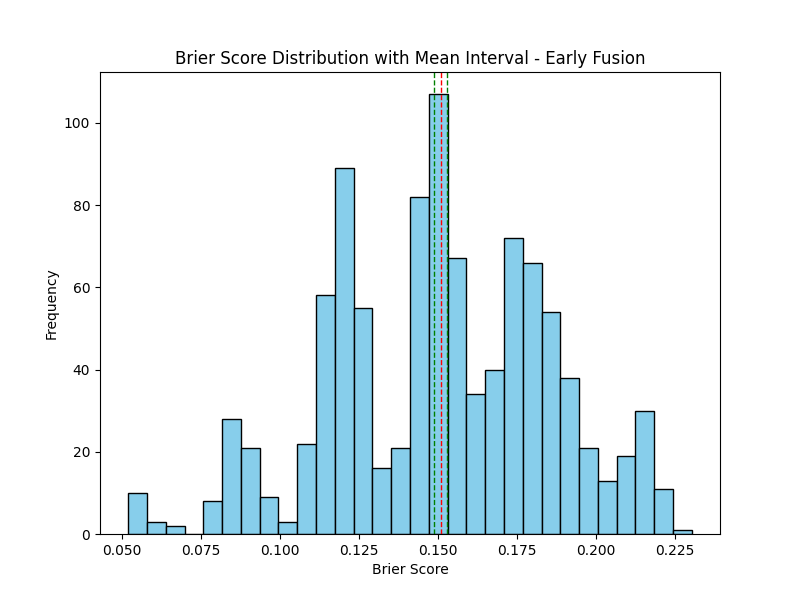
\includegraphics[width=0.5\columnwidth]{figs/early_fusion.png}}
  \subfloat[] 
  {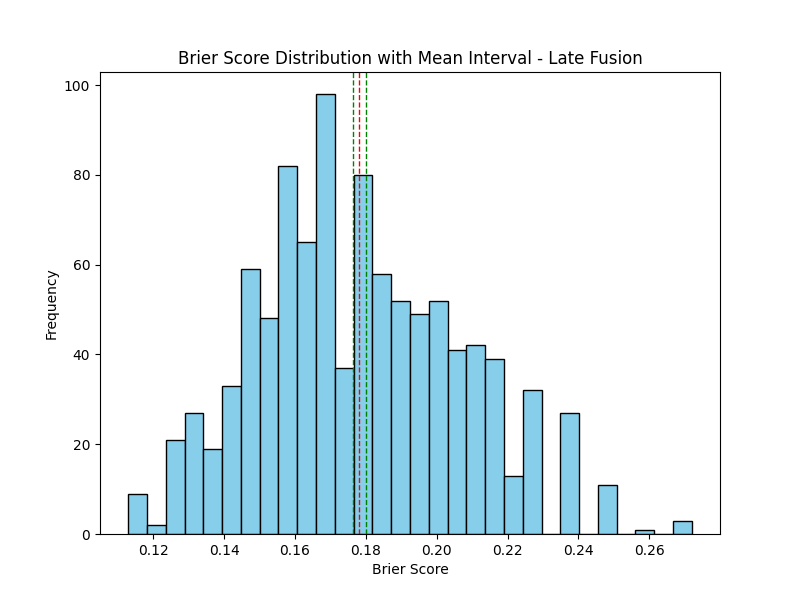
\includegraphics[width=0.5\columnwidth]{figs/late_fusion.png}}
  \caption{NOODLE's Brier score (a) Early fusion (b) Late fusion}
  \label{fig:gan}
\end{figure*}

\begin{figure*}[]
\centering
\begin{minipage}{0.30\textwidth}
\centering
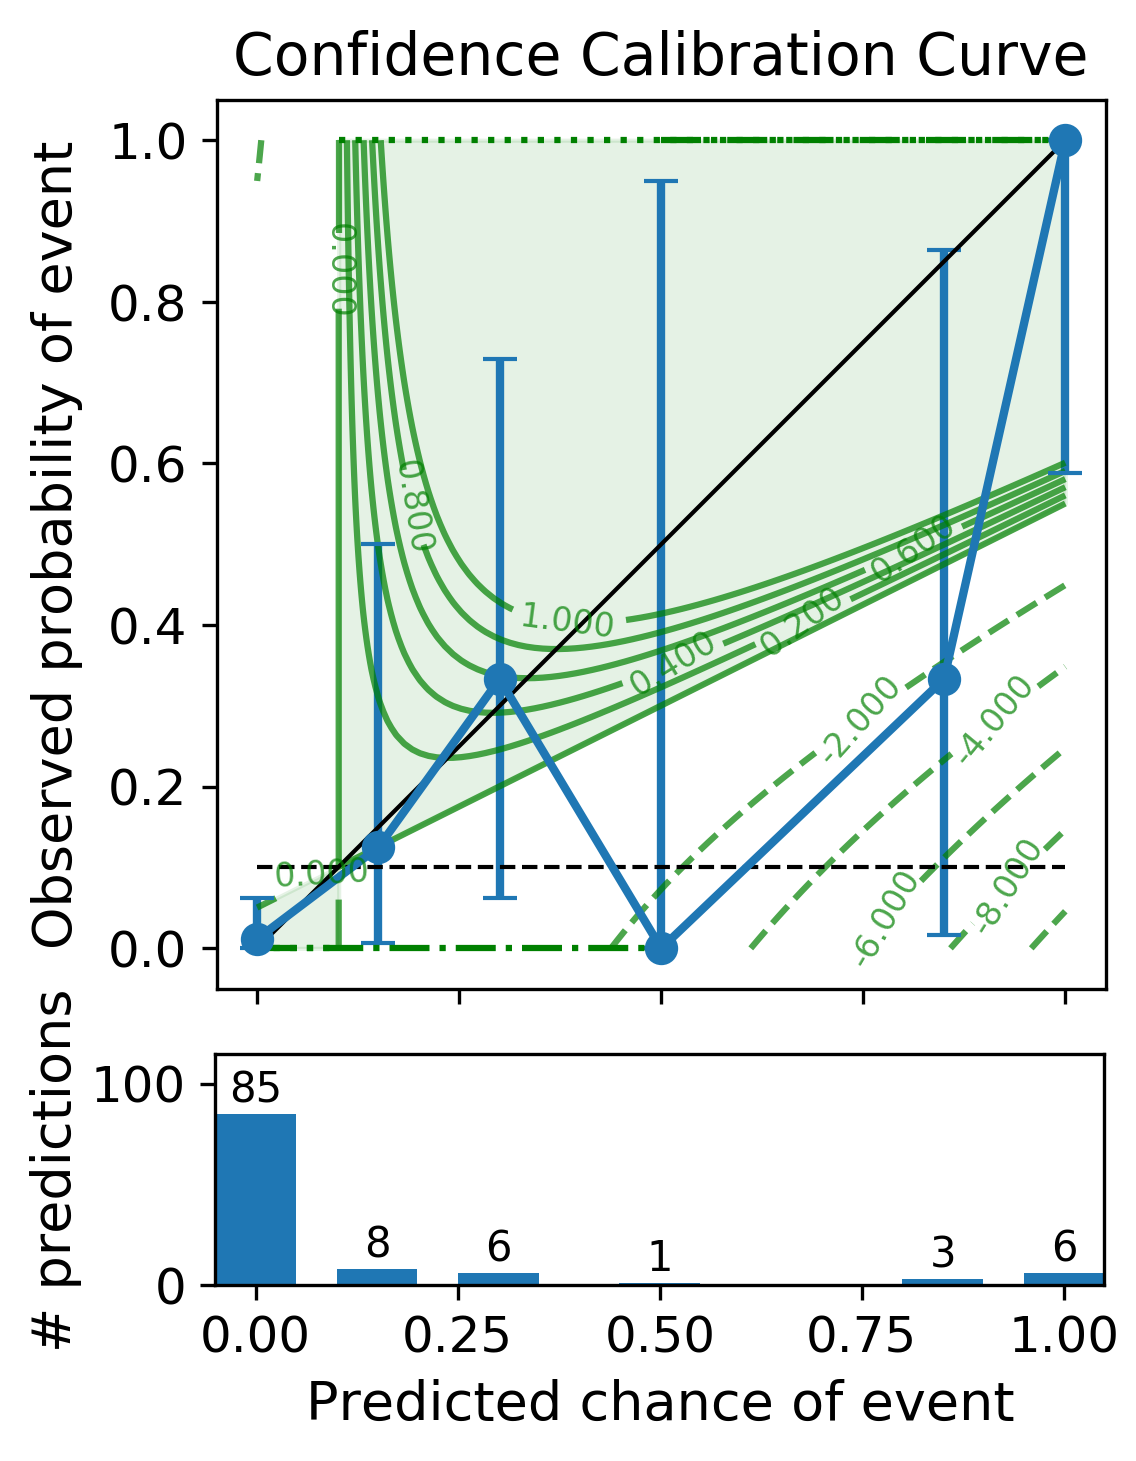
\includegraphics[width=0.79\textwidth] {figs/1.png}
\captionof{figure}{NOODLE's confidence calibration curve}
\label{fig:ccc}
\end{minipage}% 
\hspace{0.5em}
\begin{minipage}{0.30\textwidth}
\centering
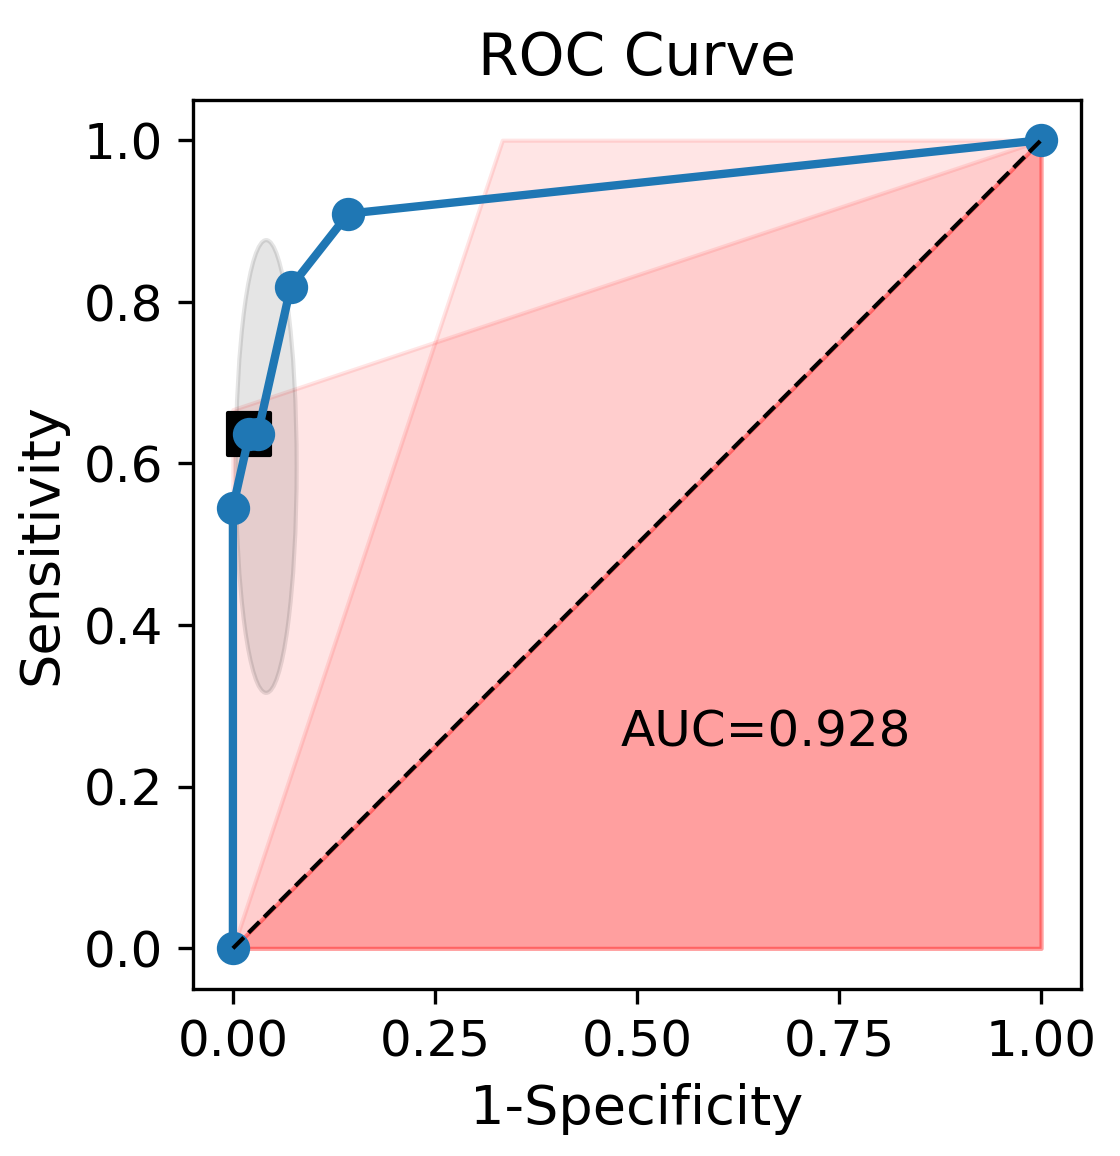
\includegraphics[width=0.98\textwidth]{figs/2.png}
\captionof{figure}{NOODLE's ROC-AUC curve under late fusion}
\label{fig:gan5}
\end{minipage}
\hspace{0.5em}
\begin{minipage}{0.35\textwidth}
\centering
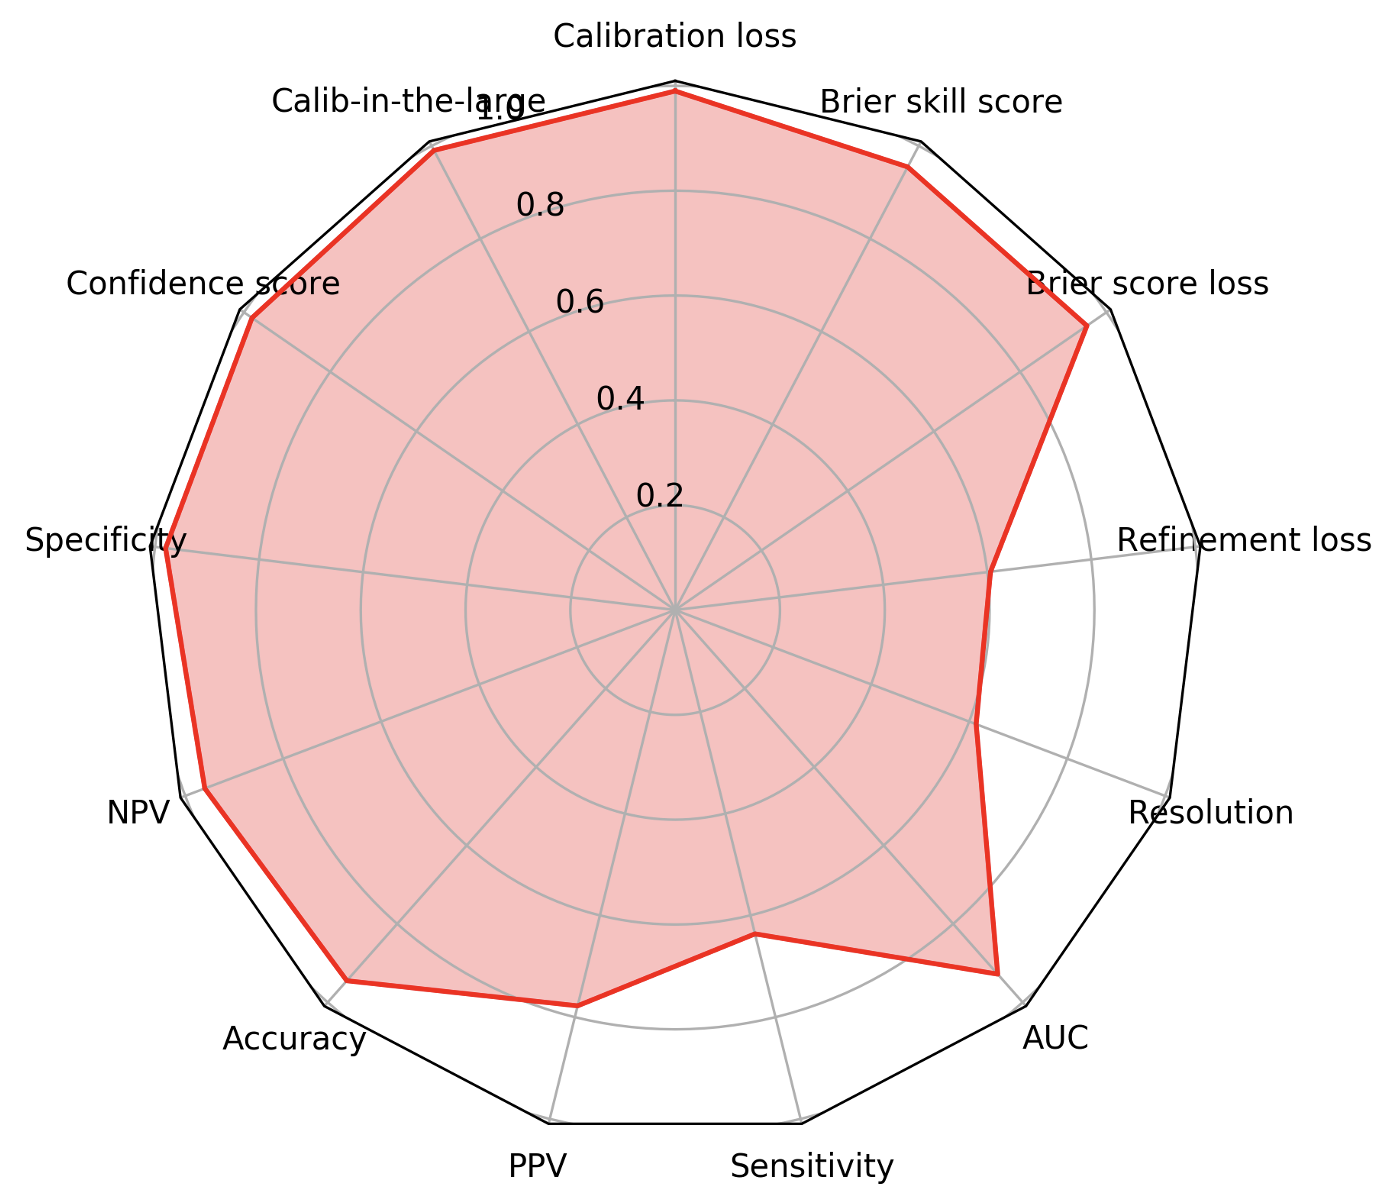
\includegraphics[width=\textwidth]{figs/radar.png}
\captionof{figure}{NOODLE's radar plot for consolidated metrics}
\label{fig:radar}
\end{minipage}
\end{figure*}

%\begin{figure}[!b]
%\centering
 % 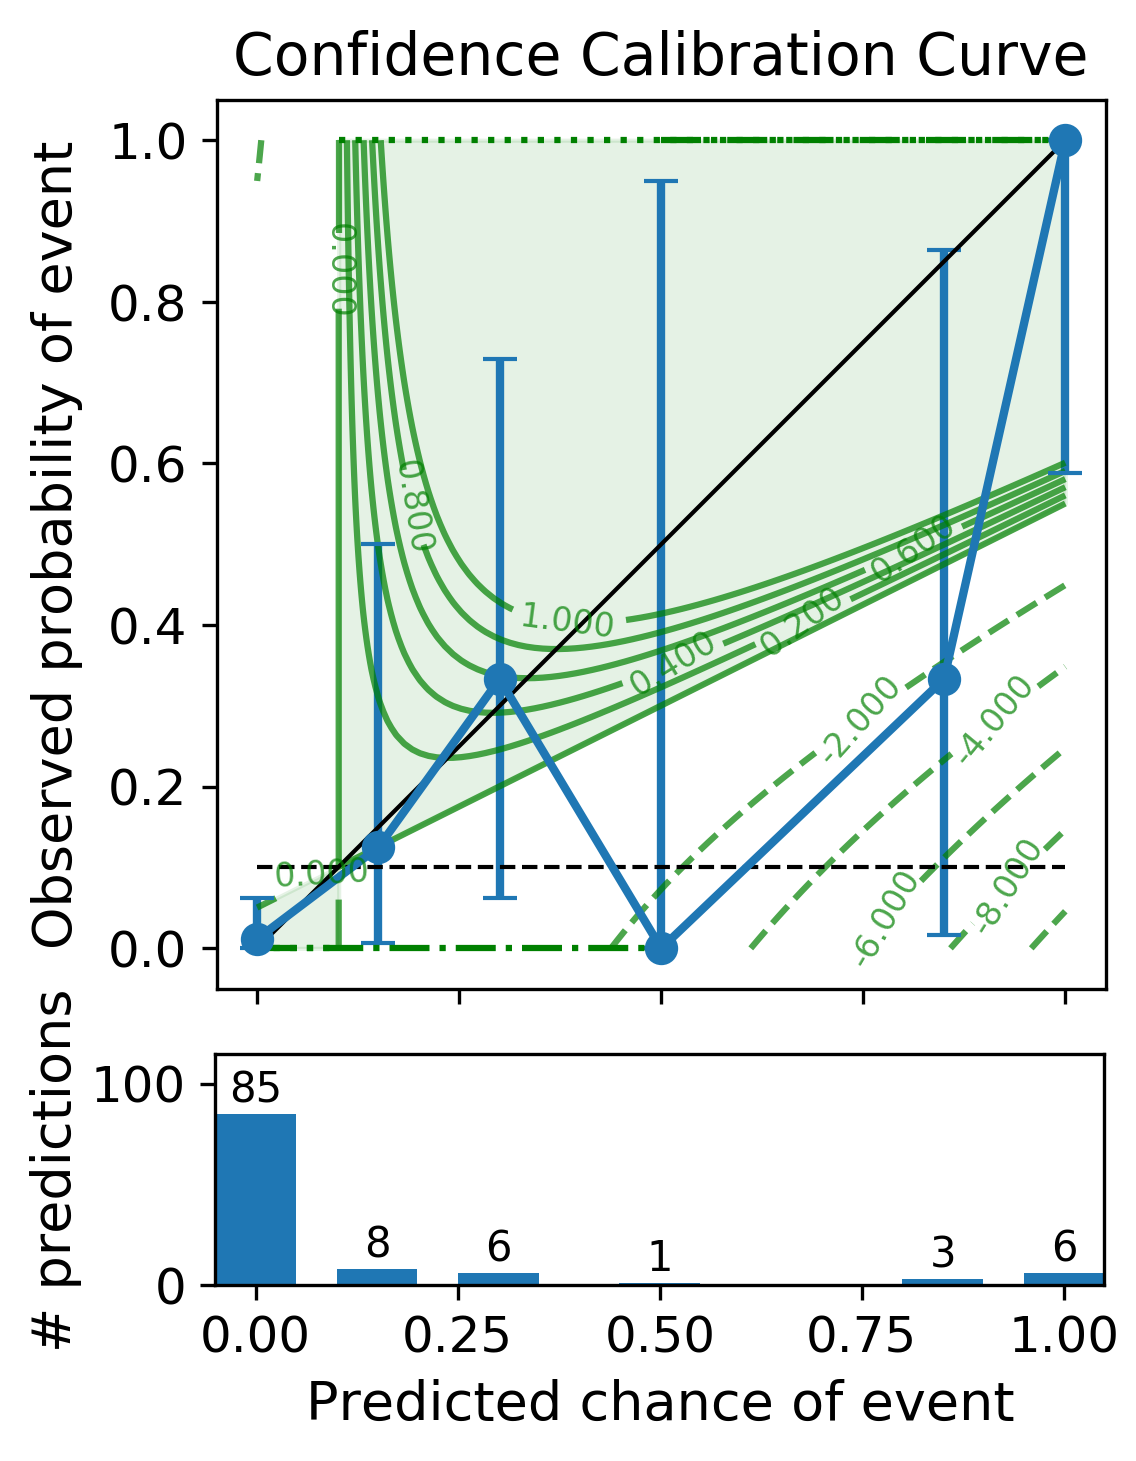
\includegraphics[width=0.7\columnwidth]{figs/1.png}
  %\caption{NOODLE's confidence calibration curve}
  %\label{fig:ccc}
%\end{figure}

We begin the evaluation process by independently assessing each modality. This involves conducting binary classification on both the graph dataset and the tabular data. The resulting comparative Brier scores for these classification tasks are presented in Table \ref{tab:table1}. The experimental outcome demonstrates that, when employing the same CNN-based deep learning model with identical hyperparameters, the graph dataset yields a superior Brier score (0.1798) compared to the tabular data (0.1913). It is worth noting that while we established a baseline model using CNN, any other alternative classification algorithms can also be employed in this context.

Then, we tested \textit{NOODLE} with two different information fusion approaches, i.e., early fusion (feature) and late fusion (decision). As shown in Table \ref{tab:table1}, the early fusion approach, which combines the graph and tabular data before processing, yields a Brier score of 0.1685. On the other hand, the late fusion strategy, which integrates the graph and table data after individual processing, demonstrated the best performance with a Brier score of 0.1589.

It is worth noting that neither of these data fusion methods can be deterministically labeled as superior \cite{gallo2017multimodal} as each one of them will demonstrate their potential to produce favorable outcomes when the data distribution changes. For this reason, we implemented both of the fusion approaches and chose the approach that provides a better Brier score (i.e., closer to 0), as mentioned in Step 8 of Algorithm \ref{algo:mdd}. The corresponding Brier score distribution with mean interval is also shown in Fig. \ref{fig:gan}a and Fig. \ref{fig:gan}b for early and late fusion, respectively. This provides a comprehensive view of predictive accuracy across multiple scenarios and is also useful for comparing models and understanding the variability in performance.

%\begin{figure}[!t]
%\centering
 % 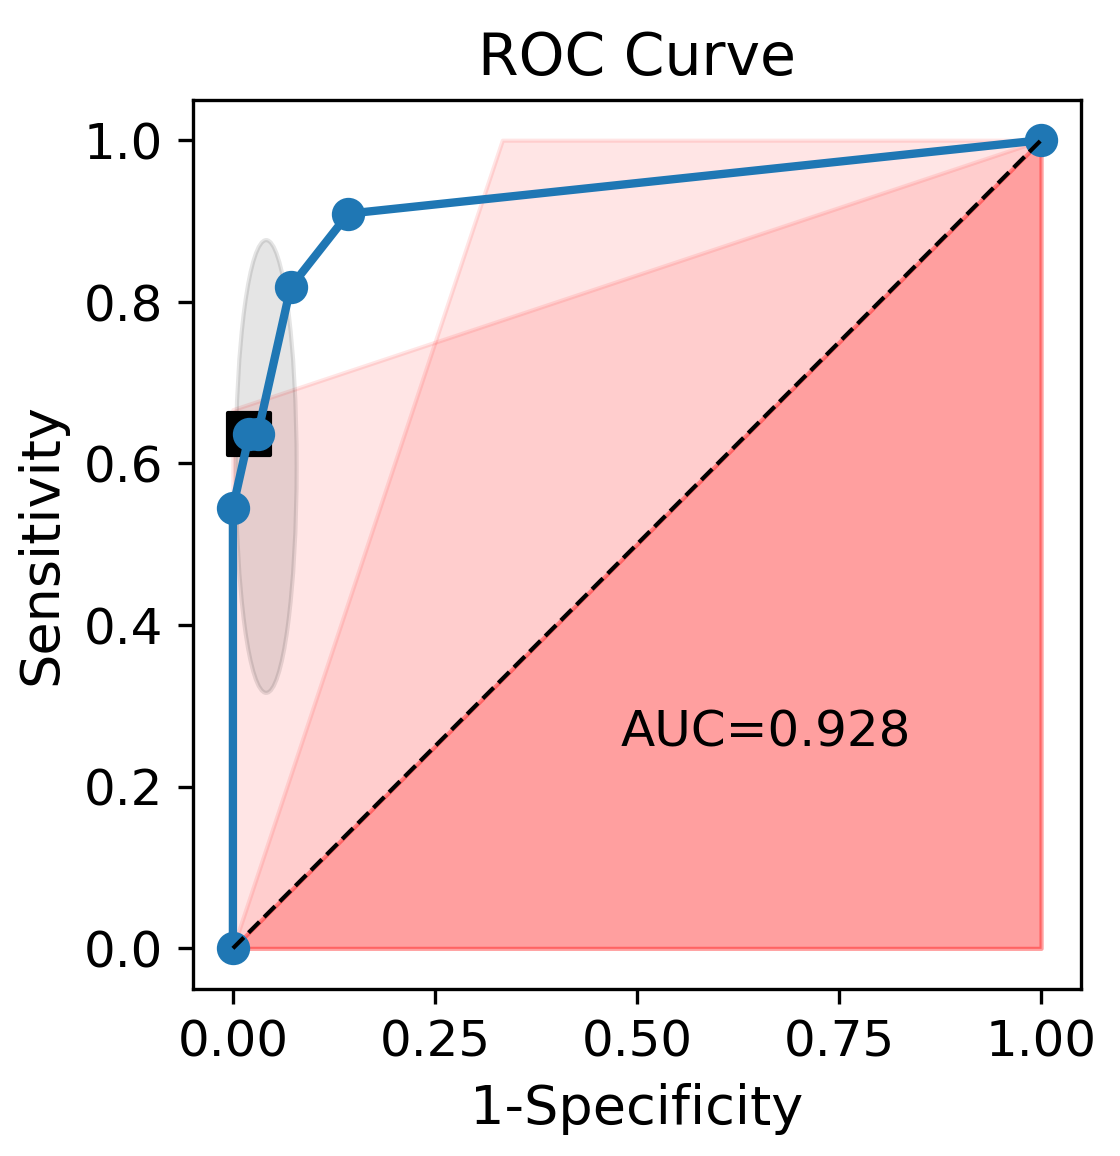
\includegraphics[width=0.7\columnwidth]{figs/2.png}
  %\caption{NOODLE's AUC-ROC curve under late fusion}
  %\label{fig:gan5}
%\end{figure}

%\begin{figure}[!b]
%\centering
 % 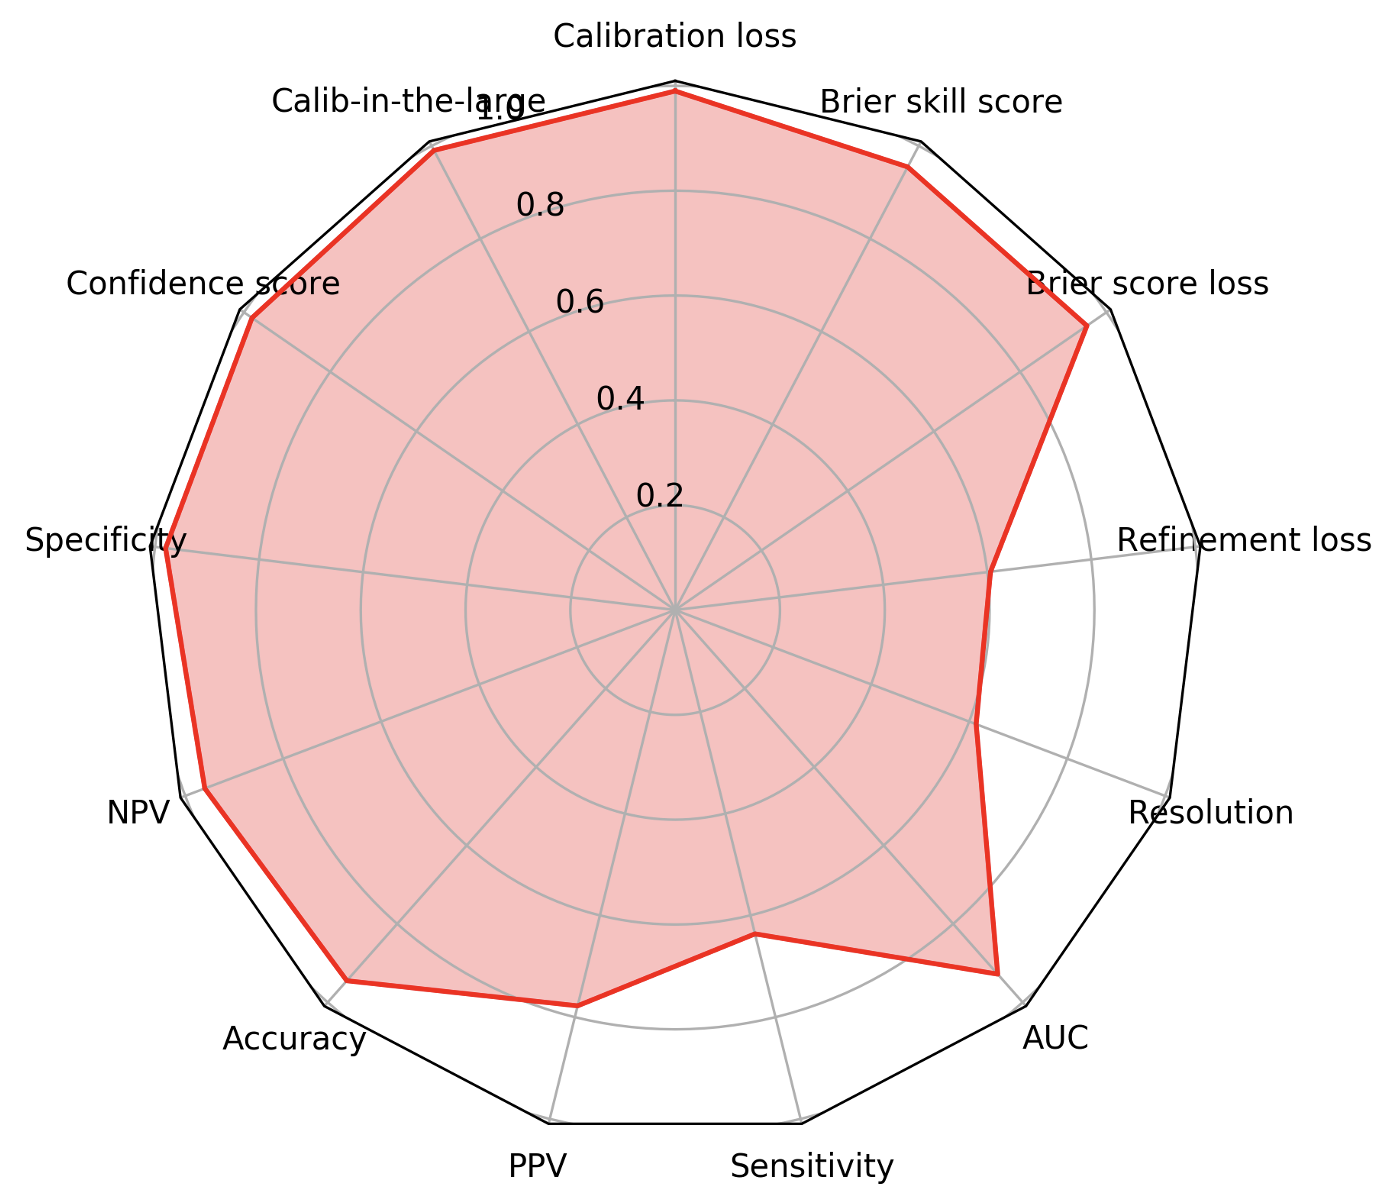
\includegraphics[width=0.8\columnwidth]{figs/radar.png}
  %\caption{NOODLE's Radar plot for consolidated metrics}
  %\label{fig:radar}
%\end{figure}


\subsection*{Confidence Calibration Curve}
The confidence calibration curve %(CCC)
plots observed probabilities of occurrence as a function of the predicted probabilities for the classification model, as shown in Fig. \ref{fig:ccc}. For the model to be perfectly calibrated, it will have all data points along the diagonal; however, in our case, the model is not well calibrated because of the highly imbalanced dataset. These are the cases on which any decision-maker should focus while making a risk-aware decision and not completely relying on accuracy alone. It helps evaluate the alignment between a model's predicted probabilities and the actual likelihood of events.

A histogram at the bottom of Fig. \ref{fig:ccc} shows the predicted chance for 109 test data. It describes the distribution of the forecasts and helps with visualization of the sharpness, i.e., tendency of the predictions to lie at the extremes of the 0-1 distribution, and is equal to the variance of the predictions.

%The curve provides crucial insights into the model's reliability, ensuring that predicted probabilities are aligned with actual probabilities for accurate decision-making.

\subsection*{ROC-AUC Curve}
The Receiver Operating Characteristic (ROC) curve illustrates the balance between sensitivity and specificity in a model. It provides a visual representation of how these two metrics change as the threshold for classifying a condition varies. The Area Under the Curve (AUC), on the other hand, quantifies the likelihood that a randomly chosen pair of circuits, one with the Trojan and one without, will be accurately classified by the model. The \textit{NOODLE}'s ROC-AUC curve is given in Fig. \ref{fig:gan5}.

The white area represents the optimal zone for model performance, and the lightly shaded red areas represent the zones of acceptable efficacy. The values for ROC-AUC range from 0 to 1, where values near `1' suggest that it can effectively discriminate between TF and TI cases with a high degree of confidence, and if the value is near `0', the model's performance is worse than random guessing. In our case, the value is 0.928, which suggests that the model is performing well.

\subsection*{Radar Plot}
The radar plot provides a visual means of presenting complex, multi-dimensional data, as shown in Fig. \ref{fig:radar}. When appraising the effectiveness of a predictor, there is a tendency to focus narrowly on a limited set of metrics. However, the radar plot provides a method for gaining a comprehensive understanding of performance across diverse dimensions. In a radar chart, each variable is represented along its corresponding axes (some variables have been normalized to conform to the 0-1 range of the radial axis). It is also important to organize the variables in a way that clusters connected ideas or principles. This aids in conducting a thorough evaluation of various facets of performance.

In the given radar plot, we have metrics related to discrimination, which include AUC, resolution, and refinement loss. Following these are combined metrics assessing both calibration and discrimination, namely the Brier score and Brier skill score. As shown in the figure, the model is less sensitive and has high accuracy. This implies that while the model is generally accurate in its predictions, it may not be as effective in identifying all the actual TI cases. This could be due to a higher number of false negatives, which means the model is missing some of the positive cases.

%%%%%%%%%%%%%%%%%%%%%%%%%%%%%%%%%%%%%%%%%%%%%%%%%%%%%
    %Discussion and Conclusion
%%%%%%%%%%%%%%%%%%%%%%%%%%%%%%%%%%%%%%%%%%%%%%%%%%%%%
\section*{Discussion}


We addressed the growing concerns related to the insertion of hardware Trojans during various stages of chip production, where confidence in fabless manufacturing is increasingly elusive. Our method involved a novel application of generative adversarial networks (GANs) to augment our dataset for missing modalities, for both graph and tabular representation of source data. Additionally, the introduction of the uncertainty-aware multimodal deep learning framework, \textit{NOODLE}, for hardware Trojan detection represented a substantial advancement. We utilized both early and late fusion strategies to thoroughly assess its efficacy. 

The deployment of multimodality and uncertainty quantification techniques showcases significant promise in addressing critical challenges within hardware security, including complexities such as logic locking. These collective contributions signify a substantial stride forward in reinforcing the security and reliability of hardware systems, especially within the evolving landscape of emerging threats.


\endgroup
\newpage

\iffalse 
\phantomsection
\addcontentsline{toc}{section}{4. SECURING CHAOTIC COMMUNICATION WITH MEMRISTORS}
\section*{Chapter 4 \\ SECURING CHAOTIC COMMUNICATION WITH MEMRISTORS}
\begingroup
\RaggedRight

\begin{quote}
``Chaos: When the present determines the future, but the approximate present does not approximately determine the future.''
\newline
\hfill  — \textit{Edward Lorenz, The Essence of Chaos}
\end{quote}

\section*{Introduction}\label{sec1}
The number of wearable devices have increased exponentially in the recent times and is expected to exceed more than \$67 Billion by 2024 \cite{9214833}. Much like embedded devices, they are loaded with sensors for collecting data from the surrounding ecosystem and transmitting the data to the destination for desired analysis and actions. With the advancement in healthcare wearable devices \cite{wang2022cloud} such as implantable pacemakers, biofluidic-based wearables, and skin-based wearables, there has been growing concern over their manufacturing and their implications for security and privacy \cite{wen2021quantum}. Consider a pacemaker as an example. If an eavesdropper gets access to the data, it creates a privacy issue for the user \cite{al2022medical}, but if the receiver's circuit is duplicated, the attacker can decode the data and pose a life-threatening threat by sending malicious actions to the pacemaker. Therefore, not only is a solution needed for reliable communication resistant to eavesdropping, but also the risk-sensitive issues of device duplication must be addressed.  

Because chaos-based communication \cite{zhong1985experimental, hedayatipour2021comprehensive} is highly sensitive to initial conditions and synchronize over time, it is a suitable choice for reliable communication \cite{duan2022fully} against eavesdroppers. Moreover, use of chaos is suggested as a potential alternative in post-quantum cryptography \cite{onuki2022secret}. Although there are improvements over chaotic communication, for example, the implementation of hyperchaotic circuits \cite{zhang2022hyperchaotic}, not much work has been done to secure the design and manufacturing of chaotic transceivers at an untrusted foundry \cite{rezaei2019hybrid}. Due to the growing trend in outsource manufacturing, the electronic industry must deal with various hardware threats that an untrusted foundry can pose. Since the third-party foundry has access to the circuit design, it can do a lot of unintended activities, which not only have a negative impact on the designers' revenues but, more importantly, can be risk-sensitive to end users, especially in the case of healthcare wearable and implantable devices. One approach to addressing untrusted foundries is to implement logic locking (a.k.a. logic encryption) on the circuits. Logic locking \cite{Koushanfar-LL} is a mechanism to enable the desired behavior of the circuit only when the correct key is applied to the circuit. Recently, Register-Transfer Level (RTL) locking is proposed to protect sensitive Intellectual Property (IP) semantics against untrusted entities \cite{limaye2021fortifying}. However, this approach is not suitable for mixed-signal circuits like transceivers. Moreover, different chaos-based implementations of basic logic gates to obfuscate power profiles and mitigate power analysis–based side channel attacks are proposed \cite{8383903,8383903journal}, and the concept of asymmetry in chaotic Boolean gates is exploited to lock the circuit \cite{9424321}; but the main goal of these initiatives is to use the unique features of chaos to reach hardware security goals in digital circuits rather than proposing secure and reliable mixed-signal chaotic transceivers. In addition, an approach to securing mixed-signal circuits via logic locking is proposed \cite{8715043}, which relies on logic locking of the digital portion of the mixed-signal IC such that unless the correct digital key is provided, the mixed-signal performance will be pushed outside of the acceptable specification range. However, directly locking the analog portion of the mixed-signal ICs via an analog key has not been investigated.

Thus, in this paper, we use a low-overhead yet effective approach to enable logic locking using memristors \cite{chua1971memristor} in the chaotic circuits. We believe that memristor, as the fourth fundamental two-terminal circuit element, can close the gap between reliable communication and secure manufacturing since its resistance can be programmed by the designer and not the foundry.

Fig. \ref{fig:Logic-locked} shows our proposed solution to address the issue of untrusted foundries and eavesdroppers together. On a logic-locked Chua's chaotic circuit, an input signal is encrypted and sent over a public channel. The encrypted signal is decoded at the receiver, which is also logic-locked, and only with the correct key values for the memristor can the message be successfully decoded. Because chaotic maps are highly sensitive and the key space is exponentially large, logic locking based on memristors makes it safe against an attacker attempting to duplicate the receiver without knowing the correct key value. The key contributions of this work are threefold:
\begin{itemize}
   \item Establishing reliable communication against eavesdroppers using memristor-based Chua's chaotic system;
    \item Proposing a novel logic locking mechanism based on the use of memristors as the keys for securing the circuit design against untrusted foundries;
    \item Practical realization of the proposed system on LTSpice and NI Multisim; and validating the system of equations in MATLAB Simulink.
\end{itemize}

\begin{figure}[!t]
    \centering
    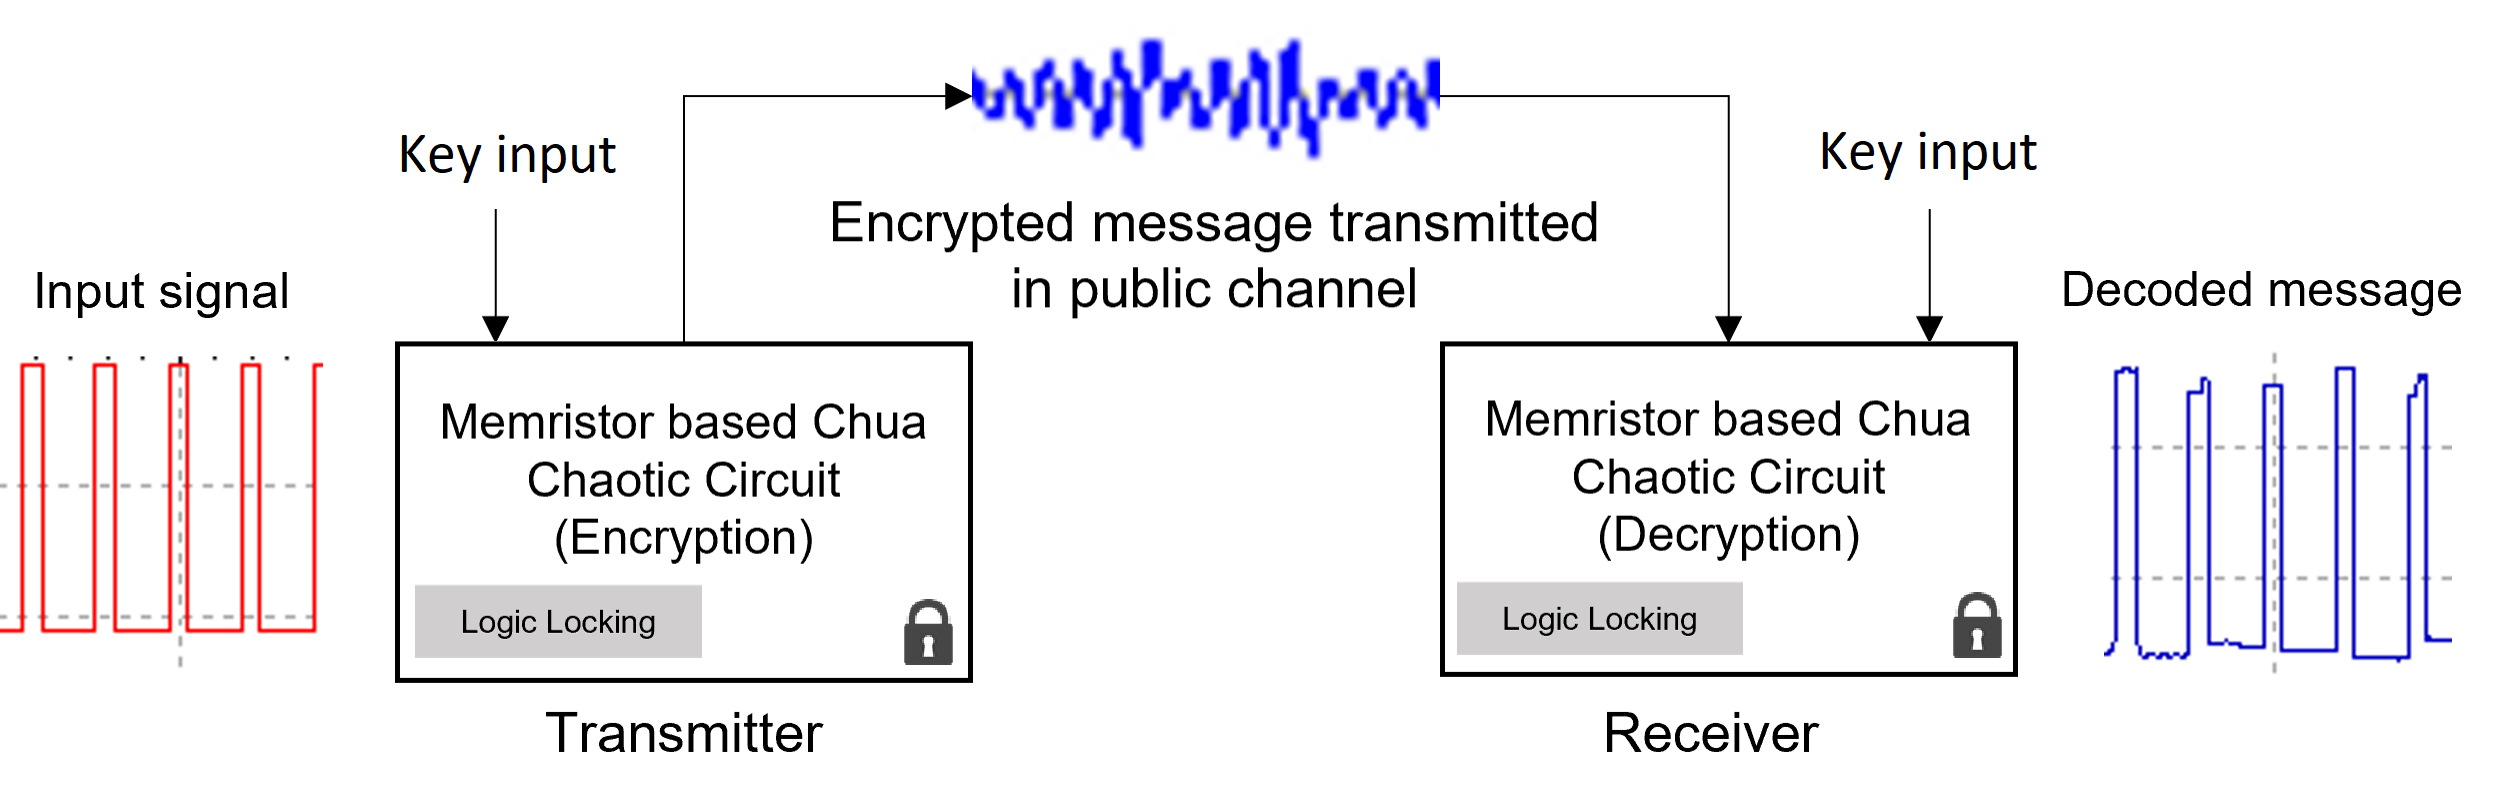
\includegraphics[width = 1\linewidth]{figs/Fig1introductionV2.png}
    \caption{Logic-locked memristor-based Chua's chaotic system}
    \label{fig:Logic-locked}
\end{figure}

The remainder of this paper is organized as follows. First, a memristor model is designed in the LTSpice Simulator in Section II. The implementation of memristor-based Chua's chaotic circuit and mathematical simulation of the circuit using MATLAB Simulink is shown in Section III. Further, in Section IV, a secure transceiver is designed using a logic-locked memristor-based chaotic circuit. Section V shows the experimental results, and the paper concludes with Section VI.

\section*{Preliminaries}\label{prelim}


\subsection*{Attack Model}
In this paper, we consider two attack models:
\begin{itemize}
\item Eavesdropper: The attacker passively listens to transceivers' communications to gain access to transmitted information. It is a privacy threat, and in our case, the goal of the eavesdropper is to find out private information about the user who uses implementable and wearable devices. 
\item Untrusted foundry: The attacker resides in the foundry and can duplicate the transceivers. It is a security threat, and in our case, the goal of the untrusted foundry is either to make a financial profit by selling unauthorized devices to the gray market or to synchronize with authorized implementable and wearable devices to send malicious actions. 
\end{itemize}
Please note that we consider that testing will be done in-house, and thus the test/verification engineer is trusted.


\subsection*{Memristor Model}
A memristor is a two-terminal electrical component relating electric charge and magnetic flux linkage. It can be viewed as a form of non-volatile memory that is based on resistance switching, which increases the flow of current in one direction and decreases the flow of current in the opposite direction. There are primarily three types of memristor model: linear, non-linear, and threshold adaptive. To add non-linearity at the boundaries, window functions are used \cite{Joglekar-Memristor, 5934403}. We use HP Memristor Model with non-linear dopant drift for transient analysis as it offers results which are in good agreement with a part of the hitherto published experiments. A detailed implementation of the model can be found in \cite{biolek2009spice}. The total resistance of the memristor R\textsubscript{MEM} is given by the below equations.
\begin{equation}
R\textsubscript{MEM}(x) = R\textsubscript{ON} (x) + R\textsubscript{OFF} (1-x),
\end{equation}

\begin{equation}
x = \frac{w}{D}\in(0,1)     
\end{equation}

Fig. \ref{fig:memristor} shows the component model of the memristor on LTSpice XVII(x64) (17.0.34.0).
\begin{figure}[ht]
    \centering
    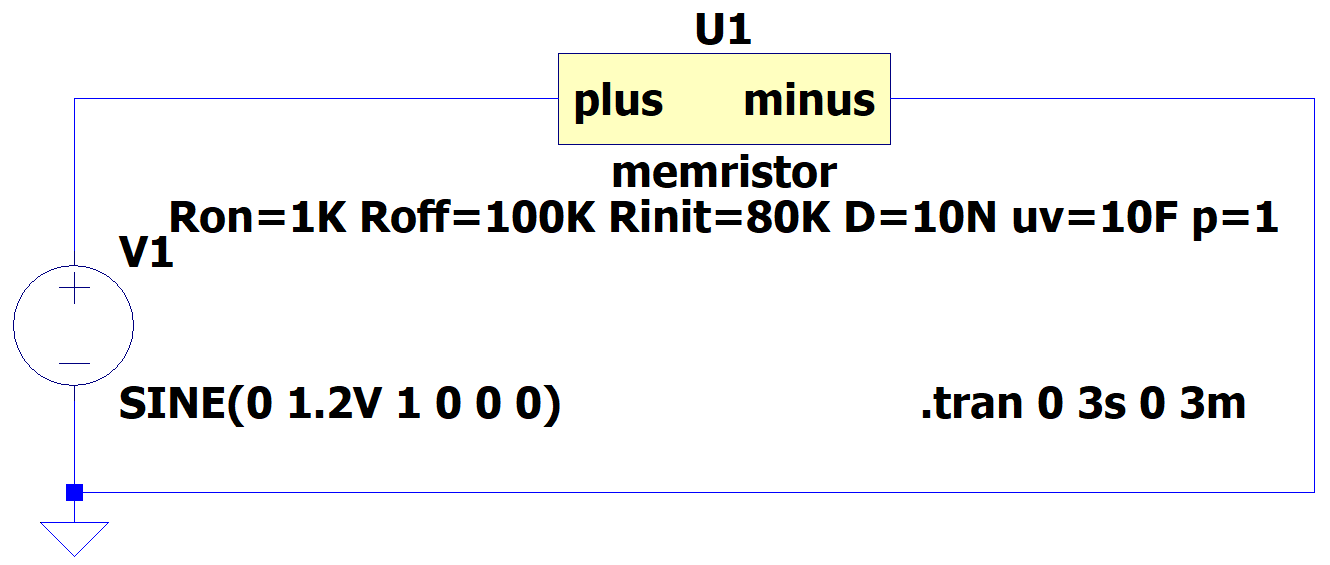
\includegraphics[width = 0.6\linewidth]{figs/Fig2memristor_model.PNG}
    \caption{Memristor component model}
    \label{fig:memristor}
\end{figure}

\subsection*{Chua's Chaotic Circuit}
Chaos can be defined as the unpredictability of a deterministic system that is highly dependent on its initial conditions. In \cite{hedayatipour2021comprehensive} different modes of chaotic equations such as Lorenz \cite{246163}, R$\ddot{o}$ssler \cite{7910544}, Chua \cite{Chua1995} and Lü \cite{ electronics10030359} have been compared for various performance metrics.

 Chua's circuit generates a chaotic behavior which is identified by a double scroll attractor or a spiral attractor. There are a few criteria for a circuit to exhibit chaotic behavior which include one or more non-linear elements, one or more resistors operating locally at the same time, and three or more energy storage elements.


 \begin{figure}[!t]
    \centering
    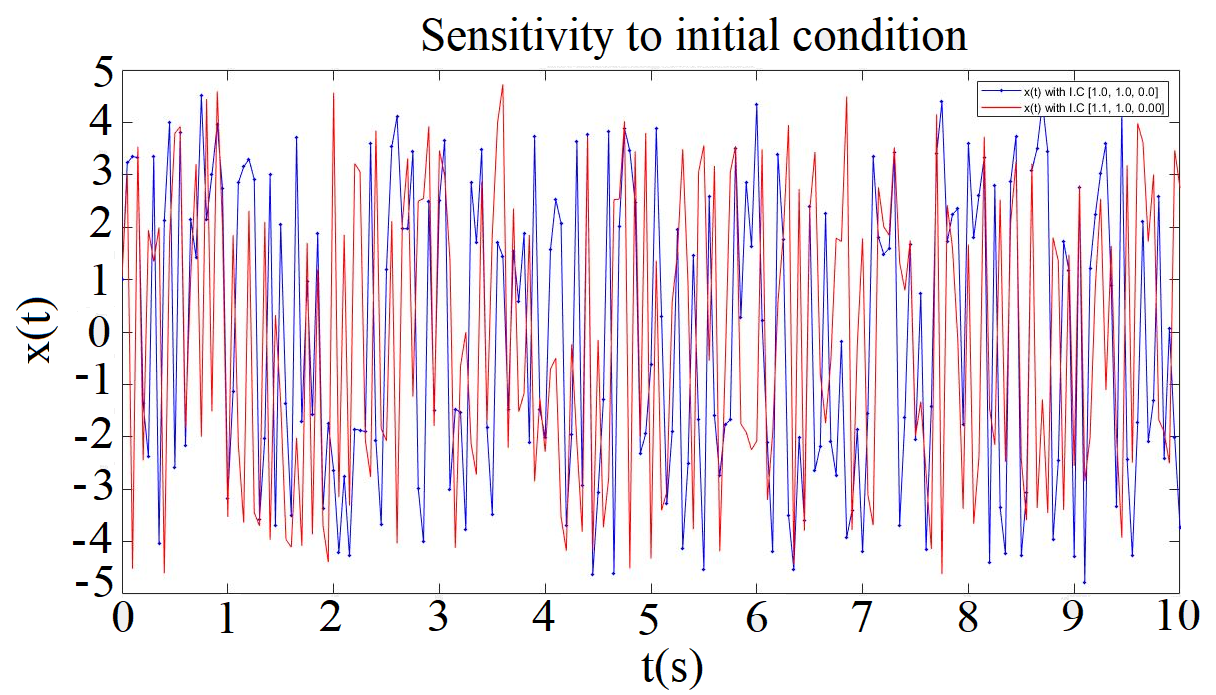
\includegraphics[width = 0.7\linewidth]{figs/Fig3Chuas_sensitivity.PNG}
    \caption{The plot of sensitivity to initial conditions of Chaos for Chua's circuit}
    \label{fig:incchua}
\end{figure}

By varying the value of one of the parameters from 1.0 to 1.1, the trajectories of x(t) are extremely
different as depicted by Fig. \ref{fig:incchua}. Thus, the Chua's circuit is the most sensitive of conventional chaotic circuits. %(Lorenz, Lü, R$\ddot{o}$ssler’s and Chua's Chaotic Equations ).
Most importantly, the Chua's circuit is one of the most basic durable experimental proofs of chaos that can be readily implemented in a variety of ways \cite{fortuna2009chua}, and provides the best performance trade-off among the others. %“one of the simplest robust experimental proof of chaos and can be easily implemented in different ways” \cite{fortuna2009chua}. 

As presented in Fig. \ref{fig:ltspice1}, two different design for Chua's chaotic equations are implemented to study the behaviour. Fig. \ref{fig:ltspice1} (a) demonstrate the design with inductor (L) valued 28mH and Fig. \ref{fig:ltspice1} (b) represents the design with the reduced inductance using the additional non-inverting amplifiers. The inductance of the circuit on the left C2 in Fig. \ref{fig:ltspice1} (b) can be calculated as below. 
    \begin{figure}[!t]
        \centering
        \subfloat[\centering ]{{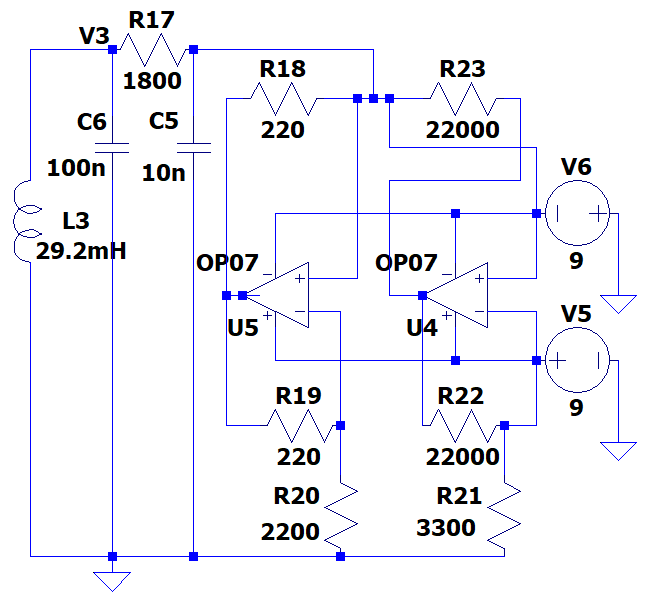
\includegraphics[scale=0.29]{figs/Fig4ach3_Chua's1st_design.PNG} }}%
        \qquad
        \subfloat[\centering ]{{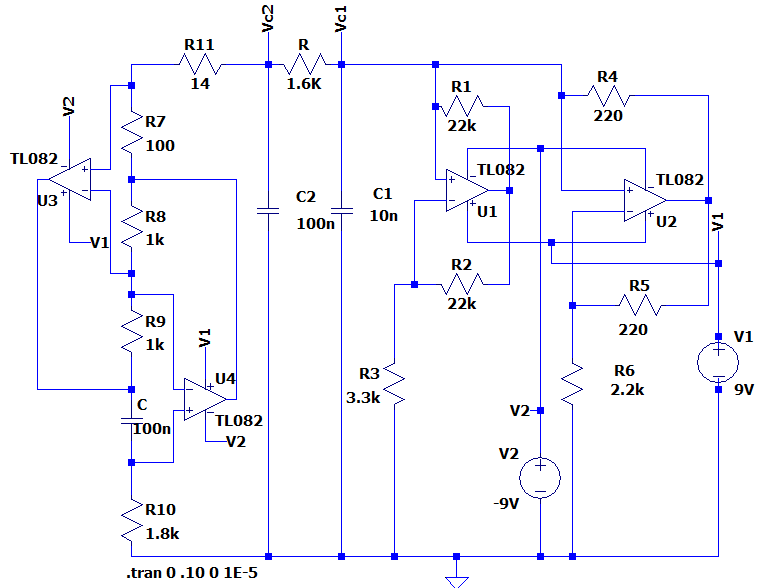
\includegraphics[scale=0.29]{figs/Fig4bch3_Chua's2nd_design.PNG} }}%
        \qquad
        \subfloat[\centering ]{{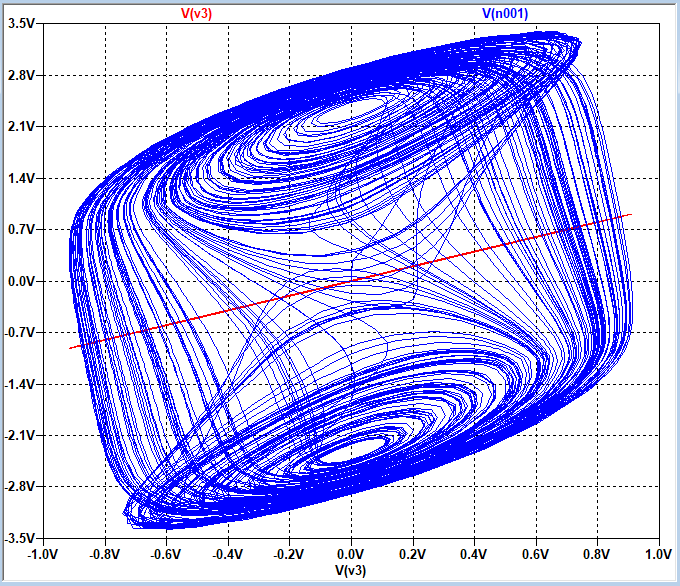
\includegraphics[height=5cm, width=5cm]{figs/Fig4cch3_Chua's1st_sim.PNG} }}%
        \qquad
        \subfloat[\centering ]{{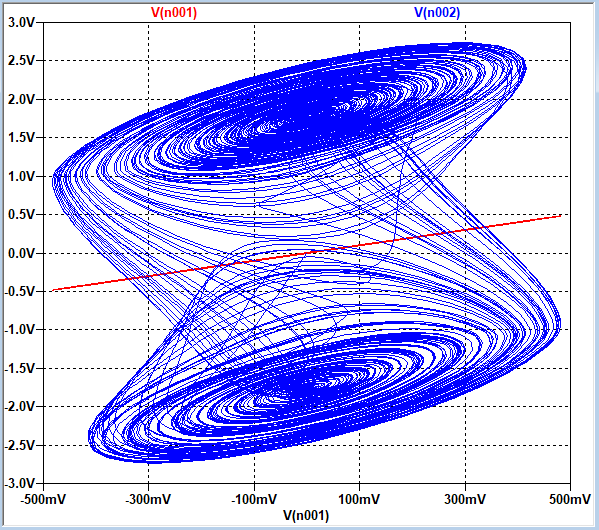
\includegraphics[height=5cm, width=5cm]{figs/Fig4dch3_Chua's2nd_sim.PNG} }}%
        \vspace{2pt}
        \caption {LTSpice design of Chau's chaos (a) with Inductor (L), (b) without Inductor (L). The attractor (c) corresponds to design in (a), and (d) corresponds to design in (b).}
        \label{fig:ltspice1}%
    \end{figure}
   % \vspace{-0.5cm}
%\[\centerline{L = (R7 * R9 * R10 * C) / R8 }  \]

\begin{equation*}
L = \frac{R7 \times R9 \times R10 \times C}{R8}    
\end{equation*}

The simulation of these LTSpice designs is shown in Fig. \ref{fig:ltspice1} (c) and (d) for designs in (a) and (b) respectively, generating Chua's attractor shape. However, the fine distinction can be observed even though they both develop Chua's attractor. The basic building block of these designs is non-inverting Operational Amplifier (Op-Amp).

In communication when the signal is discussed, it always important to pay attention to the noise component involved within the signal. Signal to Noise Ration (SNR) is the ratio of signal power compared to all other electrical signals, which can be identified as noise. SNR can be calculated by the mean of the signal divided by the standard deviation. SNR provides very critical information about the usability of the signal. Lower SNR tend to introduce the more Gaussian noise, as signal becomes unusable. This is also called `noise floor’. During the analysis of the chaotic equations, it is observed that the chaotic signal of Chua has the SNR near to 10 dB that makes signal more prone to noise and jitter attacks. Fig. \ref{fig:SNR} illustrates the SNR plot of signal X from Chua’s equation. The signal with SNR near to 10 dB can be identified as noise and the signal becomes unusable. The characteristic of these
chaotic equations is that it generates a signal as similar characteristic as noise signal even with
a message decoded in it. Thus, when transmitted through public channels these signals are just noise. Chua attains more chaos with parameter sensitivity, that symbolizes
the robustness of the chaotic equations to the static noise and eliminates possibilities of data loss.

\begin{figure}[!t]
    \centering
    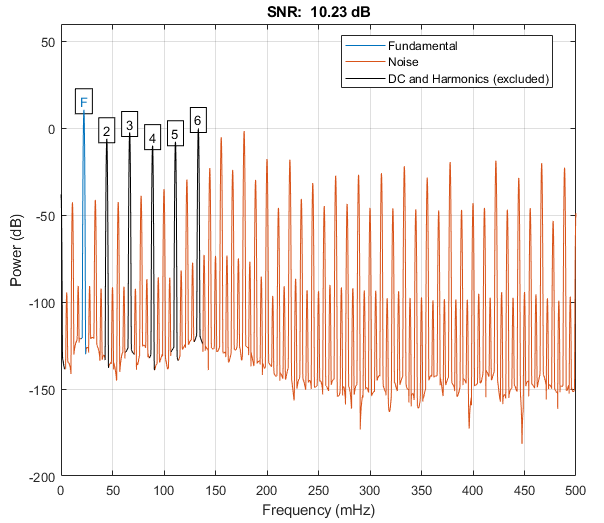
\includegraphics[width = 0.6\linewidth]{figs/Fig5SNR_chuaX.PNG}
    \caption{Signal to Noise Ratio (SNR) for Chua’s signal X}
    \label{fig:SNR}
\end{figure}


\section*{Memristor-based Chua's Chaotic Circuit}

The implementation of memristor-based Chua's chaotic circuit is described in \cite{muthuswamy2010implementing} and the same chaotic circuit is implemented using two memristors in \cite{bao2017two}. In this work, to increase the key space, we have used more than two memristors in Chua's chaotic circuit. 

\subsection*{Circuit Design in LTSpice}
Usually, for the non-linear element, a Chua's diode is utilized; however, we have used a memristor instead of a Chua's diode and also replaced a few other resistors with memristors as shown in Fig. \ref{fig:3}.

\begin{figure}[!t]
    \centering
    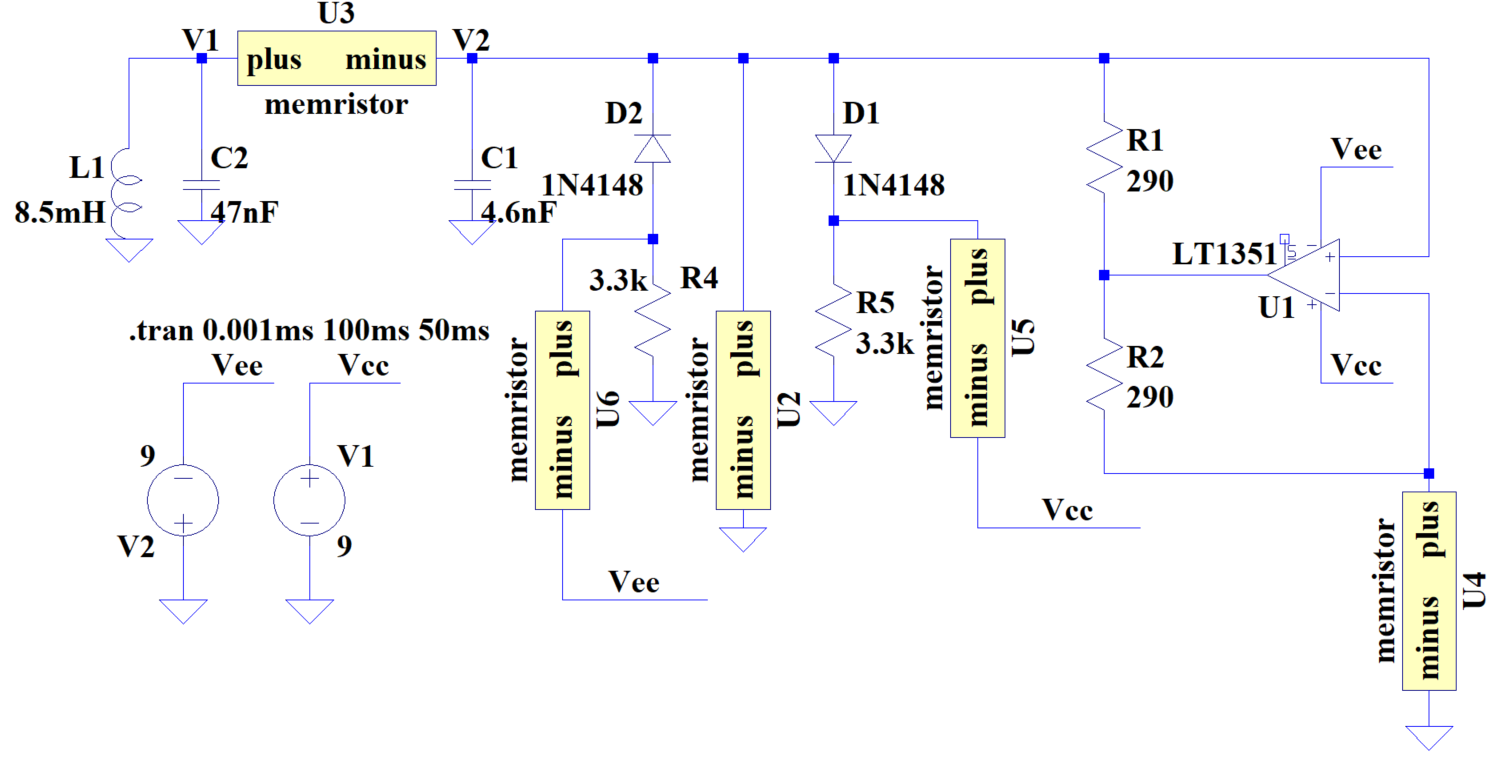
\includegraphics[width = 0.9\linewidth]{figs/Fig6chua_memristor_LTSpice.PNG}
    \caption{Implementation of memristor-based Chua's chaotic circuit}
    \label{fig:3}
\end{figure}

\begin{figure}[!t]
    \centering
    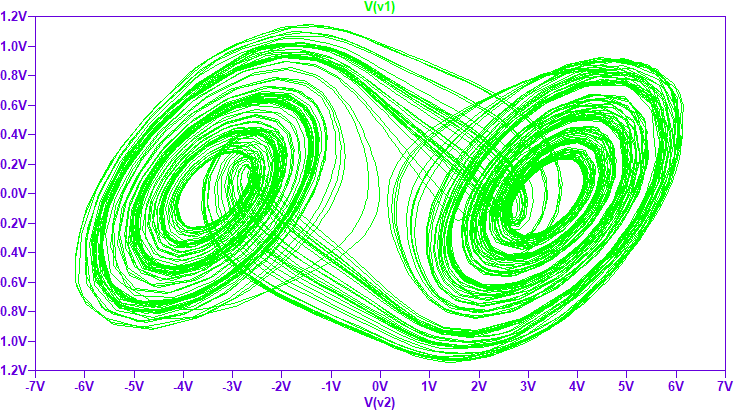
\includegraphics[width = 0.5\linewidth]{figs/Fig7double_scroll_attractor.PNG}
    \caption{Double scroll attractor for memristor U3 in Chua's chaotic circuit with values R$_{on}$=0.8K R$_{off}$=1.65K R$_{init}$=1.65K D=70N uv=10F p=1}
    \label{fig:4}
\end{figure}

\begin{figure*}[]
    \centering
    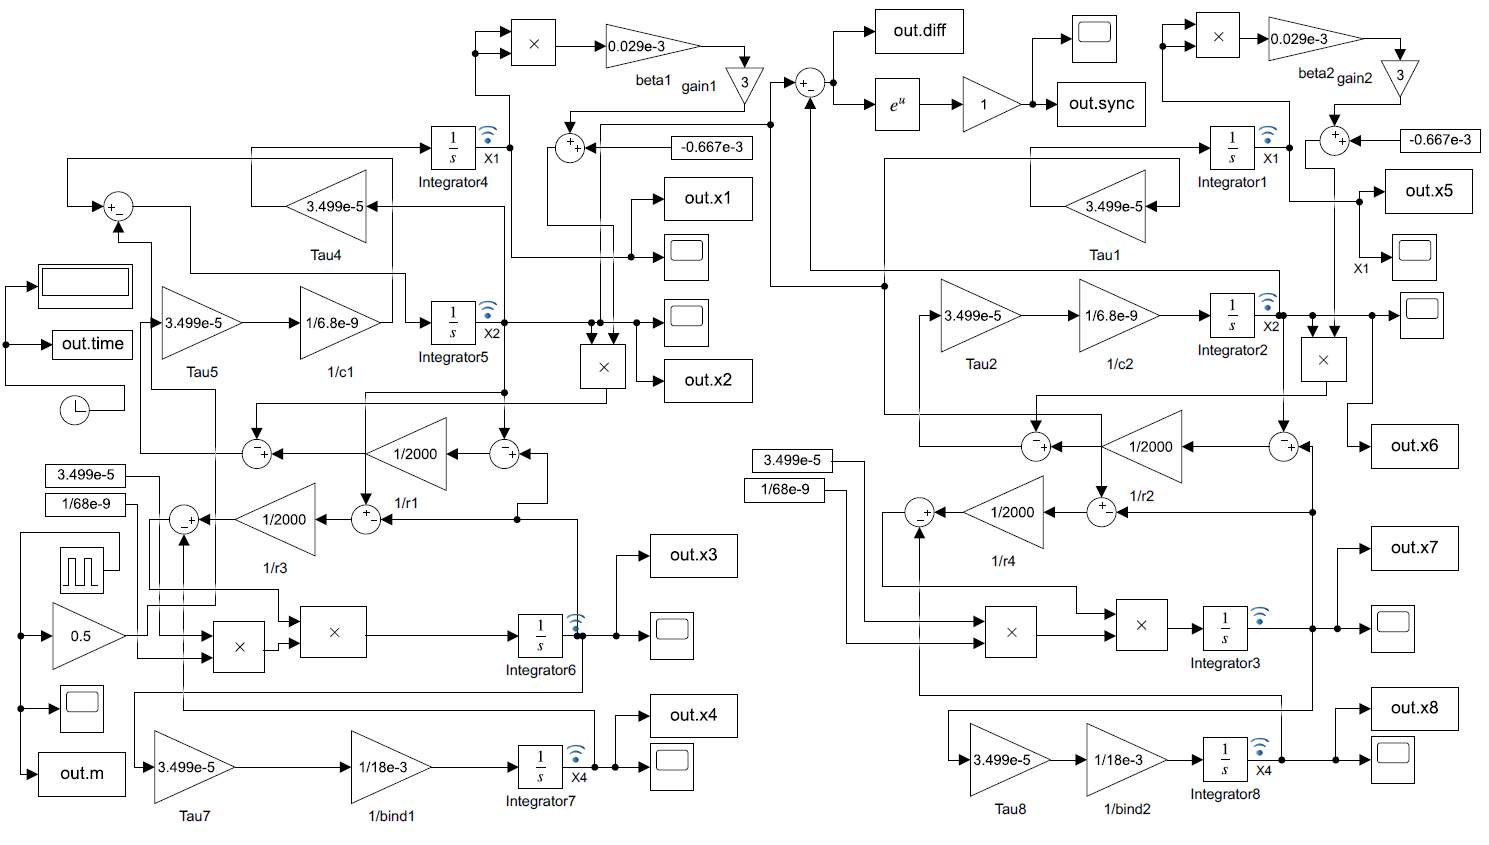
\includegraphics[width = 1\linewidth]{figs/Fig8output_simulink.PNG}
    \caption{Simulation of memristor-based Chua's chaotic circuit in MATLAB Simulink}
     \label{fig:5}
\end{figure*}

The chaotic behavior of our designed circuit is shown in Fig. \ref{fig:4} as a double scroll attractor by plotting I-V characteristics for memristor U3 in the circuit. The values of the other memristors are tuned in a range such that they satisfy the chaotic equations to exhibit chaotic behavior.


\subsection*{Mathematical Model in MATLAB Simulink}
Most of the researchers have focused on designing a system to reliably transmit the information from the sender to receiver \cite{guo2022novel} by making improvement in the way chaotic circuit is designed. For example, \cite{yang2014exponential} studies the synchronization of chaotic circuit for discontinuous chaotic systems, and \cite{9630142} uses time-scaling chaotic shift keying encryption for wireless systems. Based on the introduction of a non-linear element, i.e., memristor in the Chua's chaotic circuit, we derived the following system of equation by applying Kirchhoff Law around the loop. Fig. \ref{fig:5} shows the simulation of chaotic communication using memristor-based Chua's circuit in MATLAB Simulink.
 
\begin{equation}
\frac{d\Phi}{dt} = v\textsubscript{1}
\end{equation}

\begin{equation}
\frac{dv\textsubscript{1}(t)}{dt} = \frac{1}{C\textsubscript{1}} \left( \frac{v\textsubscript{2}(t) - v\textsubscript{2}(t)} {R} - i\textsubscript{L}(t) \right)
\end{equation}

\begin{equation}
\frac{dv\textsubscript{2}(t)}{dt} = \frac{1}{C\textsubscript{2}} \left( \frac{v\textsubscript{2}(t) - v\textsubscript{2}(t)} {R} - i\textsubscript{L}(t) \right)
\end{equation}

\begin{equation}
\frac{di\textsubscript{L}(t)}{dt} = \frac{v\textsubscript{2}(t)}{L} 
\end{equation}

The Runge–Kutta method was used, using the ode45 function, with a tolerance of 1x10-9, with a sample step of 0.01 and simulating 500 seconds. Here are the initial values used in Simulink: 
r=2000.0; 
c1=6.8e-9;	
c2=68.0e-9;	
bind=18.0e-3;
alpha = -0.667D-03;
beta=0.029D-03; 
tau=3.499e-05;
cn1=tau/c1r;
cn2=tau/c2*r; 
cn3=tau/bind;
tspan = 0:0.01:500;
x1 = 0.1; 
x2 = -0.2; 
x3 = -0.003;
x4 = 0.05;

Fig. \ref{fig:6} depicts the comparison of the input signal in red and the decoded message in blue. This can be further calibrated to obtain the accurate decoded message.  

\begin{figure}[!b]
    \centering
    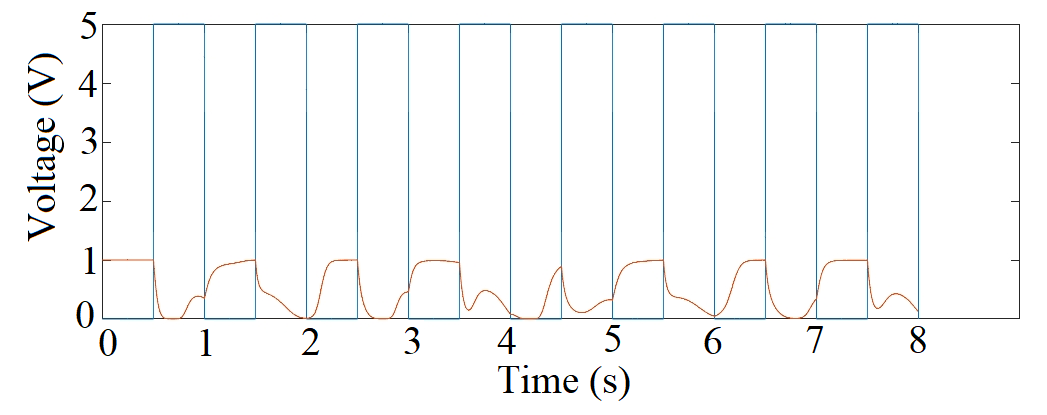
\includegraphics[width = 0.8\linewidth]{figs/Fig9syncronization.PNG}
    \caption{Comparison of input message and decoded message}
    \label{fig:6}
\end{figure}

\section*{Logic-Locked Secure Chaotic Transceivers}



With the existing research, much of the work has been done to design and improve the reliability of data transfer against eavesdroppers using chaotic communication; however, we see a gap in the security of the transceiver design itself. There can be a risk-sensitive scenario where an attacker from an untrusted foundry recreates the transceivers. To overcome this problem, we have the design goal of securing the transceivers by taking inspiration from the properties of logic locking in digital circuits. The circuit can be locked, and the locked version can be sent to the foundry for manufacturing; once the prototyped locked circuit has been returned to the design house, only the authorized users can unlock the original functionality by plugging in the secret key {\color{red}(i.e, programming the memristors based on their predefined continues values.)}

While state-of-the-art logic locking methods \cite{Koushanfar-LL,limaye2021fortifying,9427060} have focused on designing key-controlled logic gates targeted to secure purely digital circuits or designing digital keys for mixed-signal circuits \cite{8715043}, the main idea in our work is to lock the mixed-signal circuit using the analog memristors, and as we can tune the resistance value of the memristors, these continuous values can act like an analog secret key. Please note that, structurally, all the memristors used are indistinguishable, and the inside foundry attacker cannot find the value of their resistance by analyzing the circuit layout. While the key value in digital logic locking needs to be inserted into a so-called tamper-proof memory that itself may be the point of attack, here the key value is embedded into the circuit and programmed after the manufacturing.

Another part of secure and reliable communication is the design of chaotic circuits. The ``key'' values (i.e., memristors' values) will be in a certain range, which will always satisfy the chaotic equations. Although this gives a hint to the attacker to at least make an estimate of the range of values and perform the attack, even then, it will be difficult to start with brute-force as there are multiple memristors in the circuit with exponentially large key space. LTSpice model of our proposed logic-locked transmitter and receiver is shown in Fig. \ref{fig:7}. The input message is a pulse signal, which is mixed with the chaotic message, and finally it will be decoded at the receiver end. A \(\beta\)-modulator is also used in the circuit, which is a variable gain circuit designed with an inverting summing amplifier and two separate inverting amplifiers, and is controlled by a switch.

\begin{figure*}[]
    \centering
    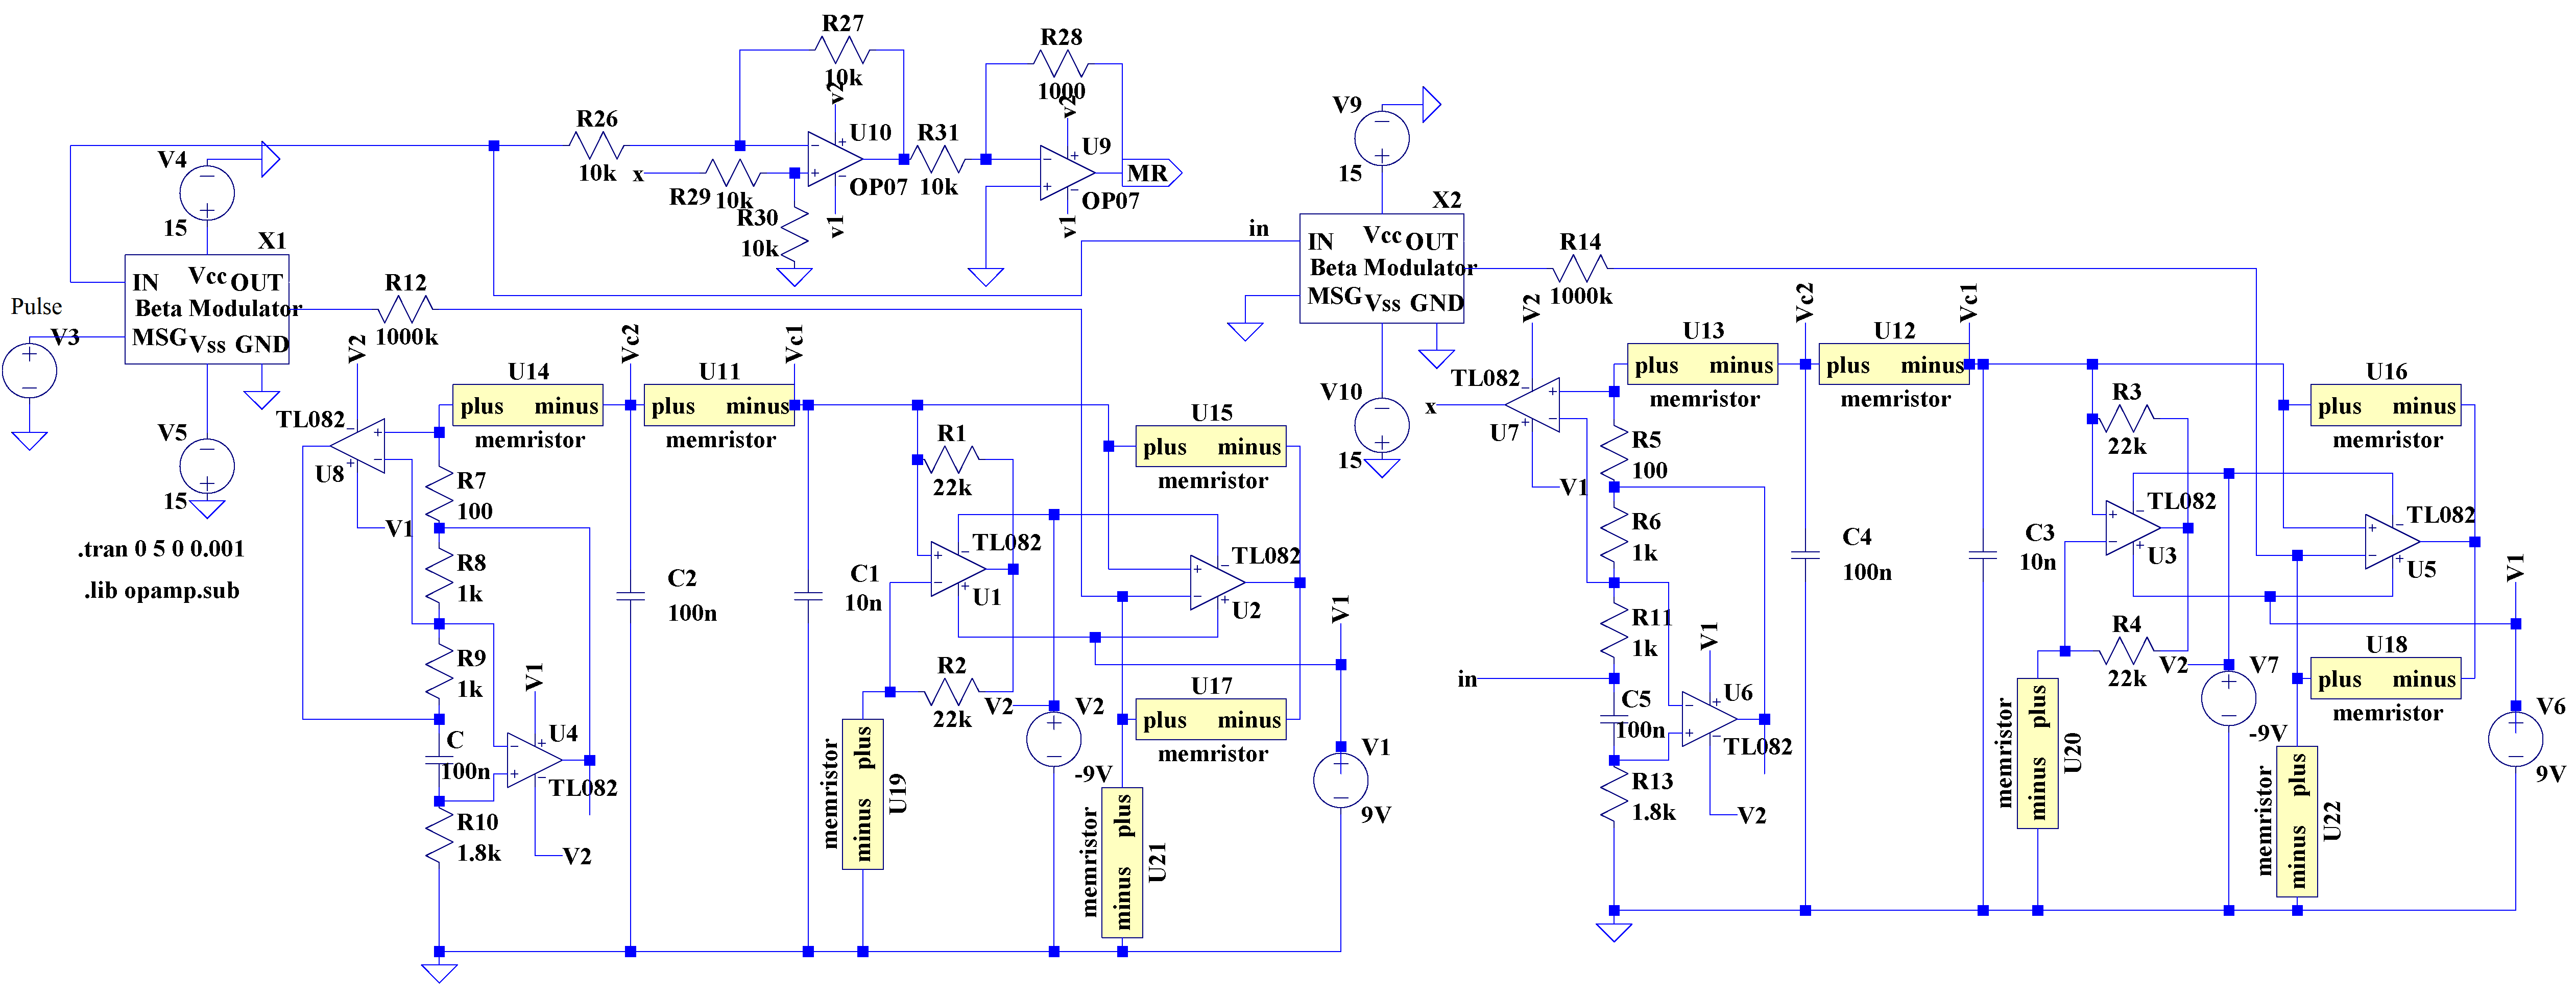
\includegraphics[width = 1\linewidth]{figs/Fig10Tx_Rx_LTSpice.PNG}
    \caption{LTSpice design of transmitter and receiver for memristor-based Chua's chaotic circuit}
     \label{fig:7}
\end{figure*}

\begin{figure}[!b]
    \centering
    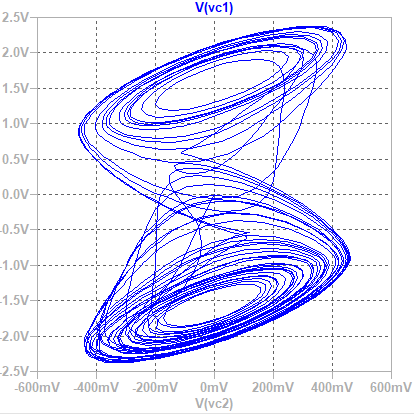
\includegraphics[width = 0.65\linewidth]{figs/Fig11double scroll attractor.PNG}
    \caption{Double scroll attractor of Chua's chaotic circuit with memristor value R\textsubscript{OFF} = 1.6K for T\textsubscript{x} (U11) and R\textsubscript{x} (U12) }
     \label{fig:8}
\end{figure}

\subsection*{Attack Analysis}
The logic locking methods designed for digital circuits with an $n$-bit key size have 2$^n$ cases with discrete values, such that R$_{i}$ $\in$ $\{0,$ 1$\}$ $\rightarrow$ 2$^n$ which cannot be broken by brute-force attack but may be challenged by the SAT-based attack \cite{7140252} that adopts a stronger attacker model by using both a locked version of the circuit and an activated transceiver bought off the market. As the SAT-based attack can handle only Boolean variables, it cannot break analog logic locking. But and advanced attack version based on satisfiability modulo theories (SMT) \cite{9000113} can be applicable here.

However, our research focuses on the use of continuous values for the keys $R\textsubscript{i}$ $\in$ $[0, R\textsubscript{max}]$ which is equivalent to the discrete form with many possibilities. Assuming we have $R\textsubscript{max}$ $=$ $m\Delta$, the above relationship can be written as $R\textsubscript{i}$ $\in$ $[0$, $\Delta$, 2$\Delta$, 3$\Delta$, ..., m$\Delta$] $\rightarrow$ m$^n$. For each memristor value, there are $m\Delta$ possibilities with $m >> n$. In comparison with the traditional method, we have m$^n$\texttt{>>}n$^n$$\texttt{>>}$2$^n$, which is double exponential.In this case, even for the SMT attack \cite{9000113}, the key size will be exponentially large, and not possible to be deciphered in polynomial time. We complement our attack analysis via experiments in Section \ref{experiments}.

\section*{Experimental results} \label{experiments}
We experimentally implemented different transceivers simulated in \cite{hedayatipour2021comprehensive} using FPGA board Nexys A7 for the system generator design of Lorenz, SprottD, and Chua as shown in Fig. \ref{fig:hwcosim2}. The parameter values, generated in XSG is taken to the MATLAB to plot them and is shown in Fig. \ref{fig:XSG}. When comparing these experimental plots with the simulation plot, it can be seen that the hardware experimental data matches the attractor shape for each equation and generates the chaos. The details of these hardware implementation is published in our recent work \cite{monani2022implementation}.

    \begin{figure}[!ht]
        \centering
        \subfloat[\centering ]{{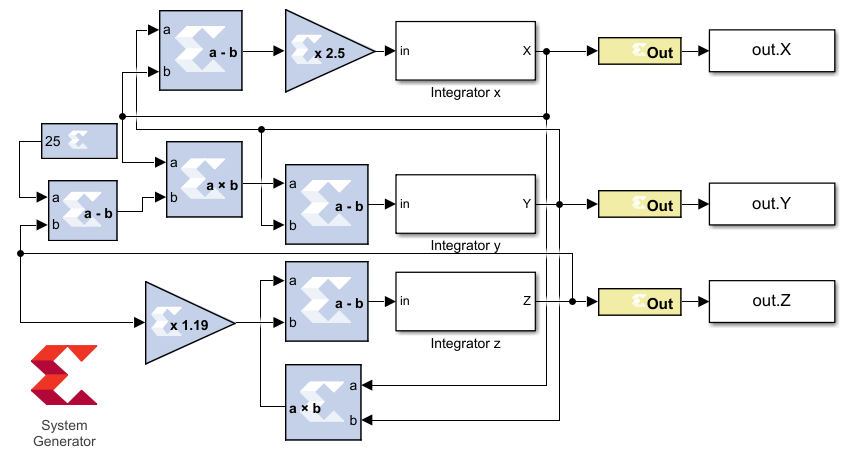
\includegraphics[height=4cm, width=7cm]{figs/Fig12aLorenz_XSG.PNG} }}%
        \qquad
        \subfloat[\centering ]{{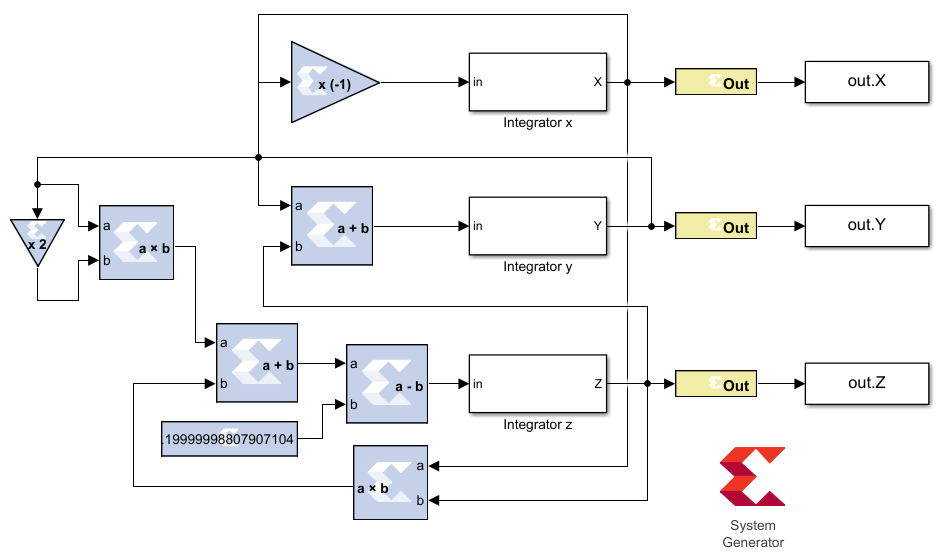
\includegraphics[height=4cm, width=7cm]{figs/Fig12bSprottD_XSG.PNG} }}%
        \qquad
        \subfloat[\centering ]{{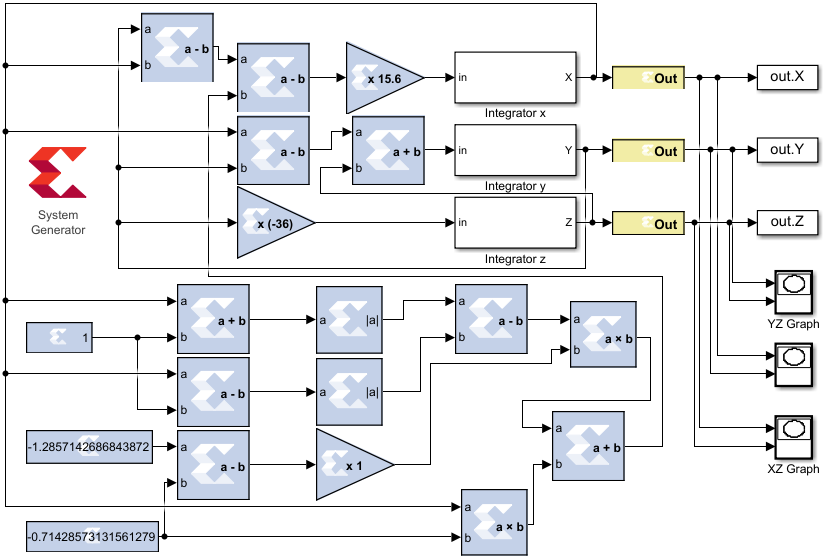
\includegraphics[scale= 0.4]{figs/Fig12cXSG_Chua.PNG} }}%
        \vspace{1pt}
        \caption{XSG Design for Transmitter of (a) Lorenz, (b) SprottD, and (c) Chua.}
        \label{fig:hwcosim2}%
    \end{figure}



        \begin{figure}[ht]
        \centering
        \subfloat[\centering ]{{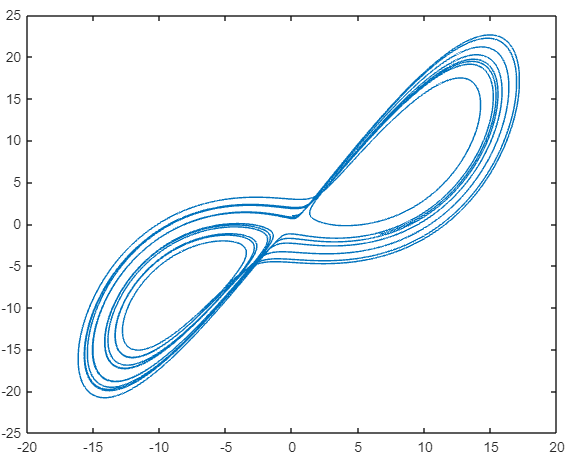
\includegraphics[height=4cm, width=4cm]{figs/Fig13aLorenz_XY_XSG.PNG} }}%
        %\qquad
        \subfloat[\centering ]{{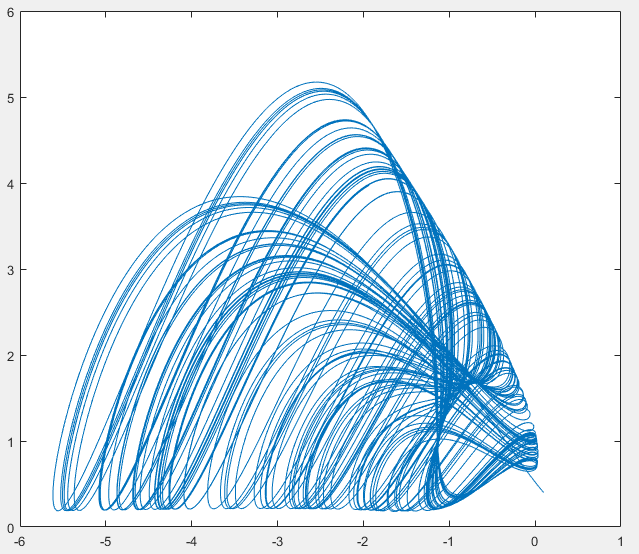
\includegraphics[height=4cm, width=4cm]{figs/Fig13bSprottD_XZ_XSG.PNG} }}%
        %\qquad \vspace{-0.2cm}
        \subfloat[\centering ]{{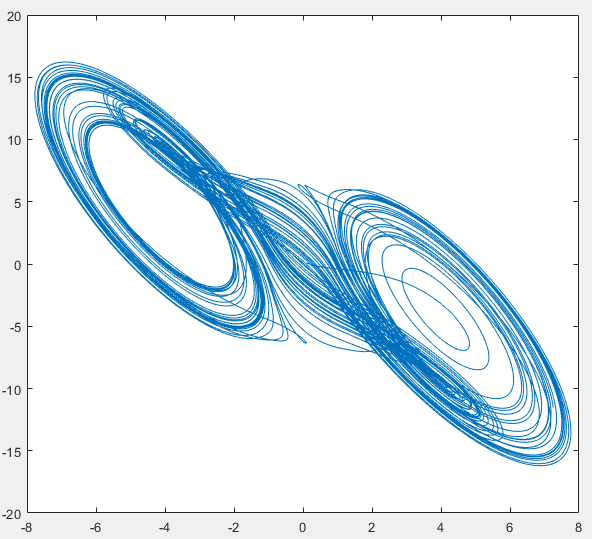
\includegraphics[height=4cm, width=4cm]{figs/Fig13cChua_XZ_XSG.PNG} }}%
       % \vspace{2pt}
        \caption{XSG hardware co-simulation plot for (a) Lorenz, (b) (SprottD), and (c) Chua.}
        \label{fig:XSG}%
    \end{figure}

The post-synthesis and the post-implementation data are represented in Table \ref{tab:resources}  for the hardware utilization. These hardware resources can be considered as Look-Up Table (LUT), Flip-Flops (FF), and Digital Signal Processors (DSP). The chart of these comparisons can also be seen in Figure \ref{fig:resource} (b).

\begin{table}[b]
	\centering
	\caption{Comparison of Resource Utilization}
	\vspace*{0.2in}
	\begin{tabular}{| c | c | c | c |c | }
		\hline
		Design & Resource & Available & Utilization & Utilization in \% \\ 
		\hline 
	Lorenz & LUT & 20800& 850 & 4.09 \\
	{} & FF & 41600& 96 & 0.23 \\
	{} & DSP & 90 & 15 & 16.67 \\
	\hline 
	SprottD & LUT & 20800& 578 & 2.78 \\
	{} & FF & 41600& 96 & 0.23 \\
    {} & DSP & 90 & 14 & 15.56 \\
    \hline
	Chua & LUT & 20800& 933 & 4.49 \\
	{} & FF & 41600& 96 & 0.23 \\
	{} & DSP & 90& 20 & 22.22 \\
		\hline
	\end{tabular}
	\label{tab:resources}
\end{table}

 \begin{figure}[t]
        \centering
        \subfloat[\centering ]{{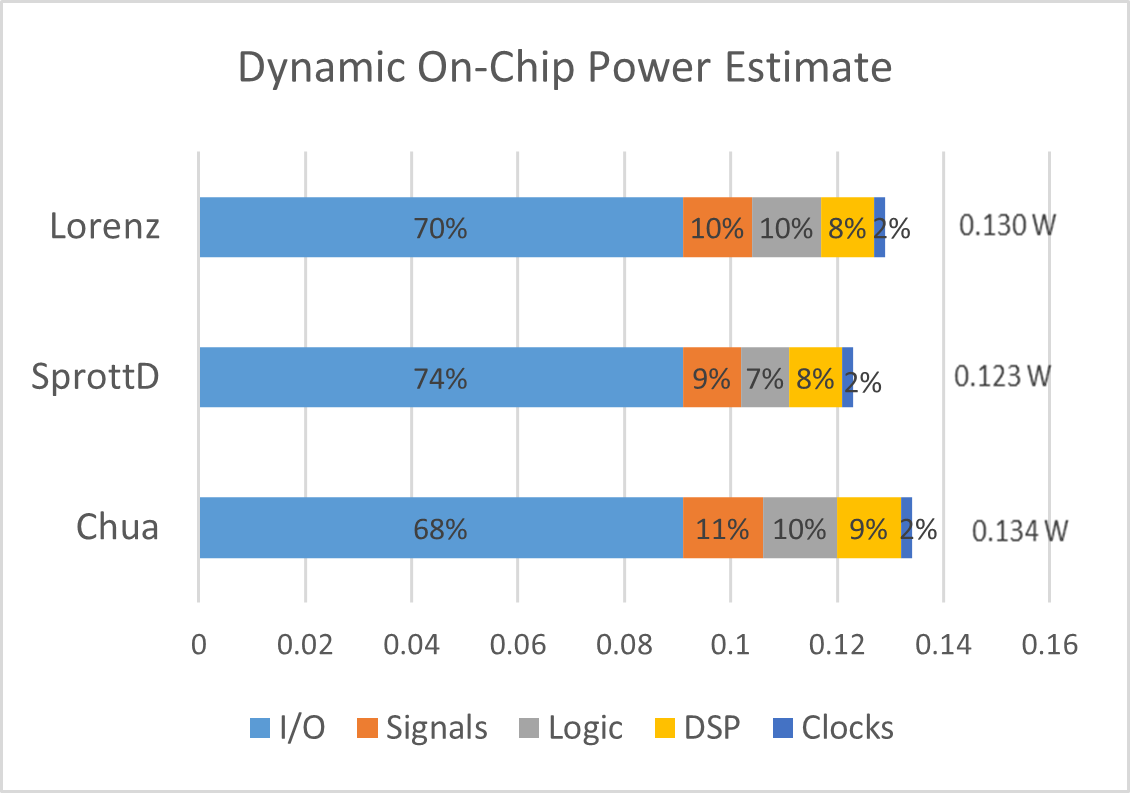
\includegraphics[height=5cm, width=7.6cm]{figs/Fig14aPower_est.png} }}%
        \qquad
        \subfloat[\centering ]{{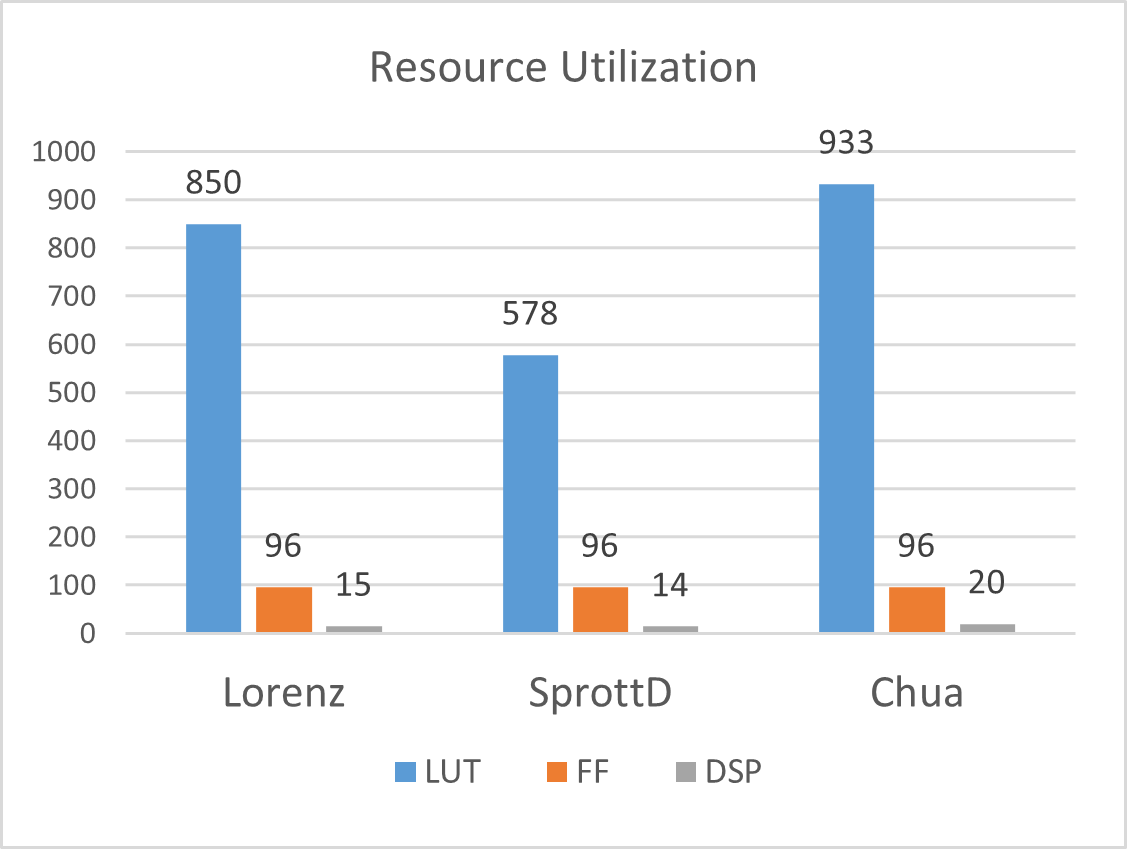
\includegraphics[height=5cm, width=7.85cm]{figs/Fig14bResource_uti.png} }}%
        \vspace{-6pt}
        \caption{Comparison of Chaotic Equation for (a) On-Chip Power Estimate, (b) Resource Utilization.}
        \label{fig:resource}%
    \end{figure}


The circuit design is shared with the untrusted foundry, and once the manufactured circuits are received, the memristor values can be tuned in-house to create a pair of transmitter and receiver that can only work together. The use of memristors secures the mechanism in that even if someone gains access to the entire circuit, the circuit will not function without the specific key inserted. On the other hand, in a situation where an eavesdropper has access to the message transmitted, he/she cannot decode the message without knowing the actual values of the memristors used in the pair of transceivers. 

Thus, for experimental validation, we will discuss two scenarios for performing chaos-based communication:
\begin{itemize}
\item \textbf{Scenario 1:} We only vary the circuit's component parameters of the transmitter, keeping the receiver's parameters constant to achieve a chaotic circuit and perform secure communication.
\item \textbf{Scenario 2:} We can have different values of the memristor component in the transmitter as well as receiver and still achieve secure communication.
\end{itemize}

\begin{figure}[!t]
    \centering
    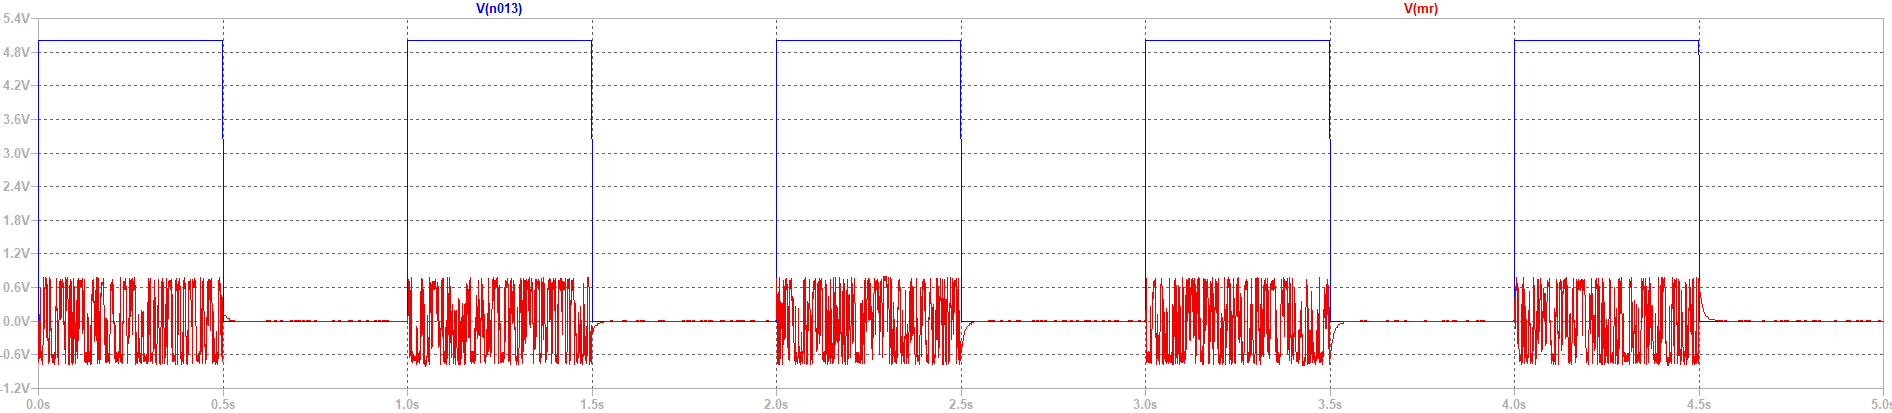
\includegraphics[width = 0.8\linewidth]{figs/Fig15U11_1_6K.PNG}
    \caption{Case 1: Original message V(n013) in blue color and decoded message V(mr) in red color}
    \label{fig:9}
\end{figure}

In the first scenario, the focus is on the chaotic circuit that can be regulated by the similar system of equations but having slightly different parameters which are in the limit of component tolerances. The second scenario focuses on the chaotic circuit with different dynamical behaviors because of the component's different parameters (parametric mismatches). Finally we also show the results of the SMT attack on our proposed transceiver in Fig. \ref{fig:7}.

\subsection*{Transmitter \& Receiver with Identical Memristors}

The two circuits, transmitter and receiver are identical, but their component's tolerance range obey the set of equations mentioned in \cite{chua1971memristor} to generate Chua's chaotic behavior. In our experiment we consider two cases and show that if the memristor's values are within the tolerance range, a secure communication is established and the encoded message is decoded successfully.  
\newline
\\
\textbf{Case 1:} Memristor parameter R\textsubscript{OFF} = 1.6K for T\textsubscript{x} (U11) and R\textsubscript{x} (U12)

The corresponding memristor values of T\textsubscript{x} and R\textsubscript{x} are set identical, but different from the suggested values mentioned in \cite{chua1971memristor}. The motive is to demonstrate large key space using memristors and establish secure and reliable chaotic communication.

\begin{center}
\small
\begin{tabular}{|c c c |} 
 \hline
 Tx & Rx & Memristor Parameters \\ [0.5ex] 
 \hline\hline
 U11 & U12 & Ron=0.8K Roff=1.6K D=70N uv=10F p=1 \\ 
 \hline
 U14 & U13 & Ron=7 Roff=14 D=70N uv=10F p=1 \\ 
 \hline
 U19 & U20 & Ron=1.65K Roff=3.3K D=70N uv=10F p=1 \\ 
 \hline
 U21 & U22 & Ron=1.1K Roff=2.2K D=70N uv=10F p=1 \\ 
 \hline
\end{tabular}
\end{center} 

The (T\textsubscript{x}, R\textsubscript{x}) memristor pairs (U11, U12), (U14, U13), (U19, U20), (U21, U22) also have a slightly different values (within the tolerance range) as mentioned in \cite{biolek2009spice} and the chaotic circuit produces a double scroll attractor as shown in Fig. \ref{fig:8}. 

Fig. \ref{fig:9} shows the decrypted signal V(mr) and is compared with the originally received signal V(n013) at the receiver end. The signal difference between them is amplified to retrieve the message signal data in order to complete the transaction. 

\textbf{Case 2:} Memristor parameter R\textsubscript{OFF} = 1.8K for T\textsubscript{x} (U11) and R\textsubscript{x} (U12)

To show that the memristor-based chaotic circuit still holds the chaotic behavior with different parameters as compared to the values used in case 1, a circuit was simulated using the below parameters of the memristors. Fig. \ref{fig:10} shows the chaotic behavior of the circuit with memristor value R\textsubscript{OFF} = 1.8K for T\textsubscript{x} (U11) and R\textsubscript{x} (U12). The comparison of input message and the decoded message is shown in Fig. \ref{fig:11}.  

\begin{center}
\small
\begin{tabular}{|c c c |} 
 \hline
 Tx & Rx & Memristor Parameters \\ [0.5ex] 
 \hline\hline
 U11 & U12 & Ron=0.9K Roff=1.8K D=70N uv=10F p=1 \\ 
 \hline
 U14 & U13 & Ron=7 Roff=13 D=70N uv=10F p=1 \\ 
 \hline
 U19 & U20 & Ron=1.65K Roff=3.2K D=70N uv=10F p=1 \\ 
 \hline
 U21 & U22 & Ron=1.1K Roff=2.19K D=70N uv=10F p=1 \\ 
 \hline
\end{tabular}
\end{center}

\begin{figure}[!b]
    \centering
    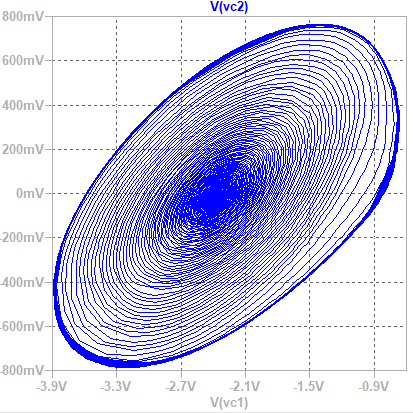
\includegraphics[width = 0.65\linewidth]{figs/Fig161_8_Spiral attractor.PNG}
    \caption{Spiral attractor of Chua's chaotic circuit with memristor value R\textsubscript{OFF} = 1.8K for T\textsubscript{x} (U11) and R\textsubscript{x} (U12)}
     \label{fig:10}
\end{figure}

\begin{figure}[!b]
    \centering
    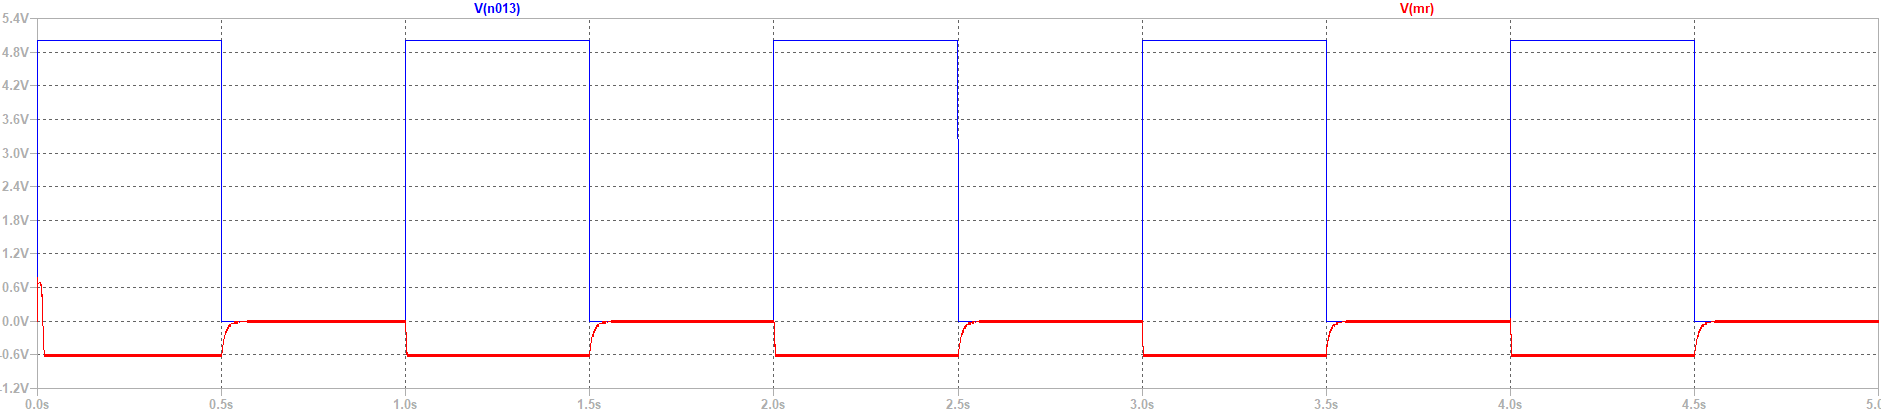
\includegraphics[width = 0.8\linewidth]{figs/Fig17U11_1_8K.PNG}
    \caption{Case 2: Original message (V(n013) in blue color and decoded message V(mr) in red color}
     \label{fig:11}
\end{figure}

Further, if the values of the memristor is changed beyond the tolerance range for which it stops exhibiting chaotic behavior, it is observed in Fig. \ref{fig:12} that the transceiver fails to decode the message.   
If we change the value of R\textsubscript{x} (U12) from Ron=0.9K Roff=1.8K D=70N uv=10F p=1 to Ron=0.9K Roff=1.79K D=70N uv=10F p=1, the message will not be decoded. So, the attacker has to be aware of all the values of the memristors present in the transmitter circuit. 

\begin{figure}[ht]
    \centering
    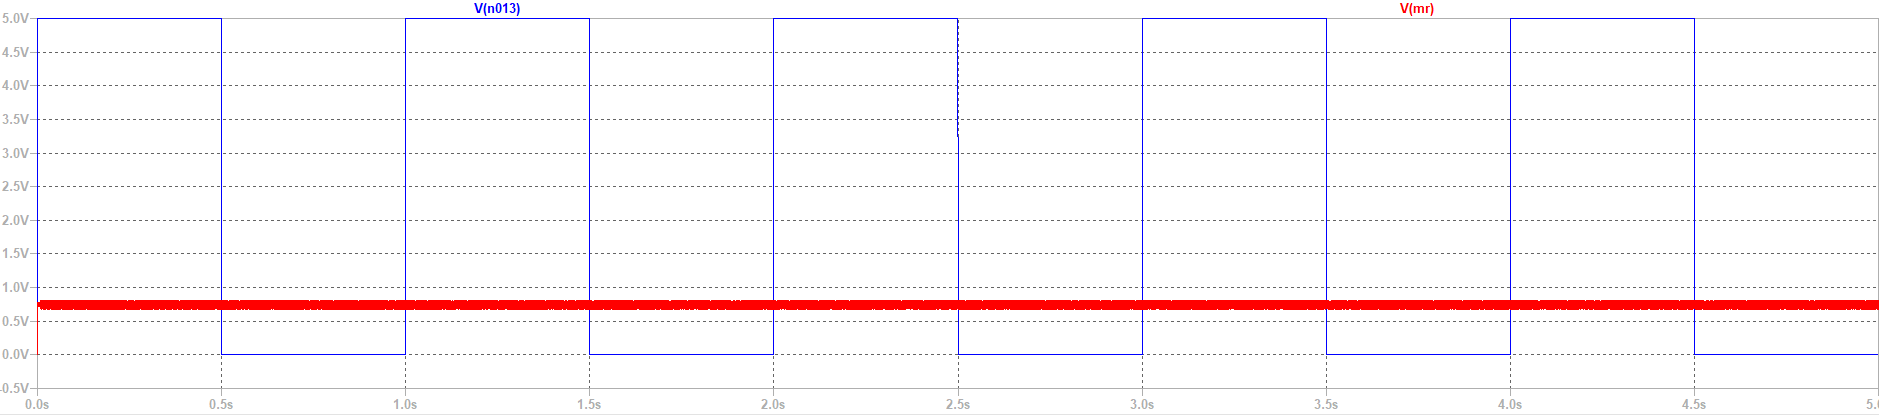
\includegraphics[width = 0.8\linewidth]{figs/Fig18U11_1_8K_no_decode.PNG}
    \caption{Message is not decoded if the memristors values are changed beyond the tolerance}
    \label{fig:12}
\end{figure}

\subsection*{Transmitter and Receiver with Non-Identical Memristors}
Second scenario is to validate if the original message is decoded at the receiver end when the Chua's chaotic circuit are non-identical, i.e., parameter mismatch. For simplicity, only one memristor value is different in transmitter and receiver, and other values of the memristor are identical. %NI Multisim 14.3 is used for designing memristor-based Chua's chaotic circuit and perform secure communication.  



\begin{figure}[!t]    
\centering
    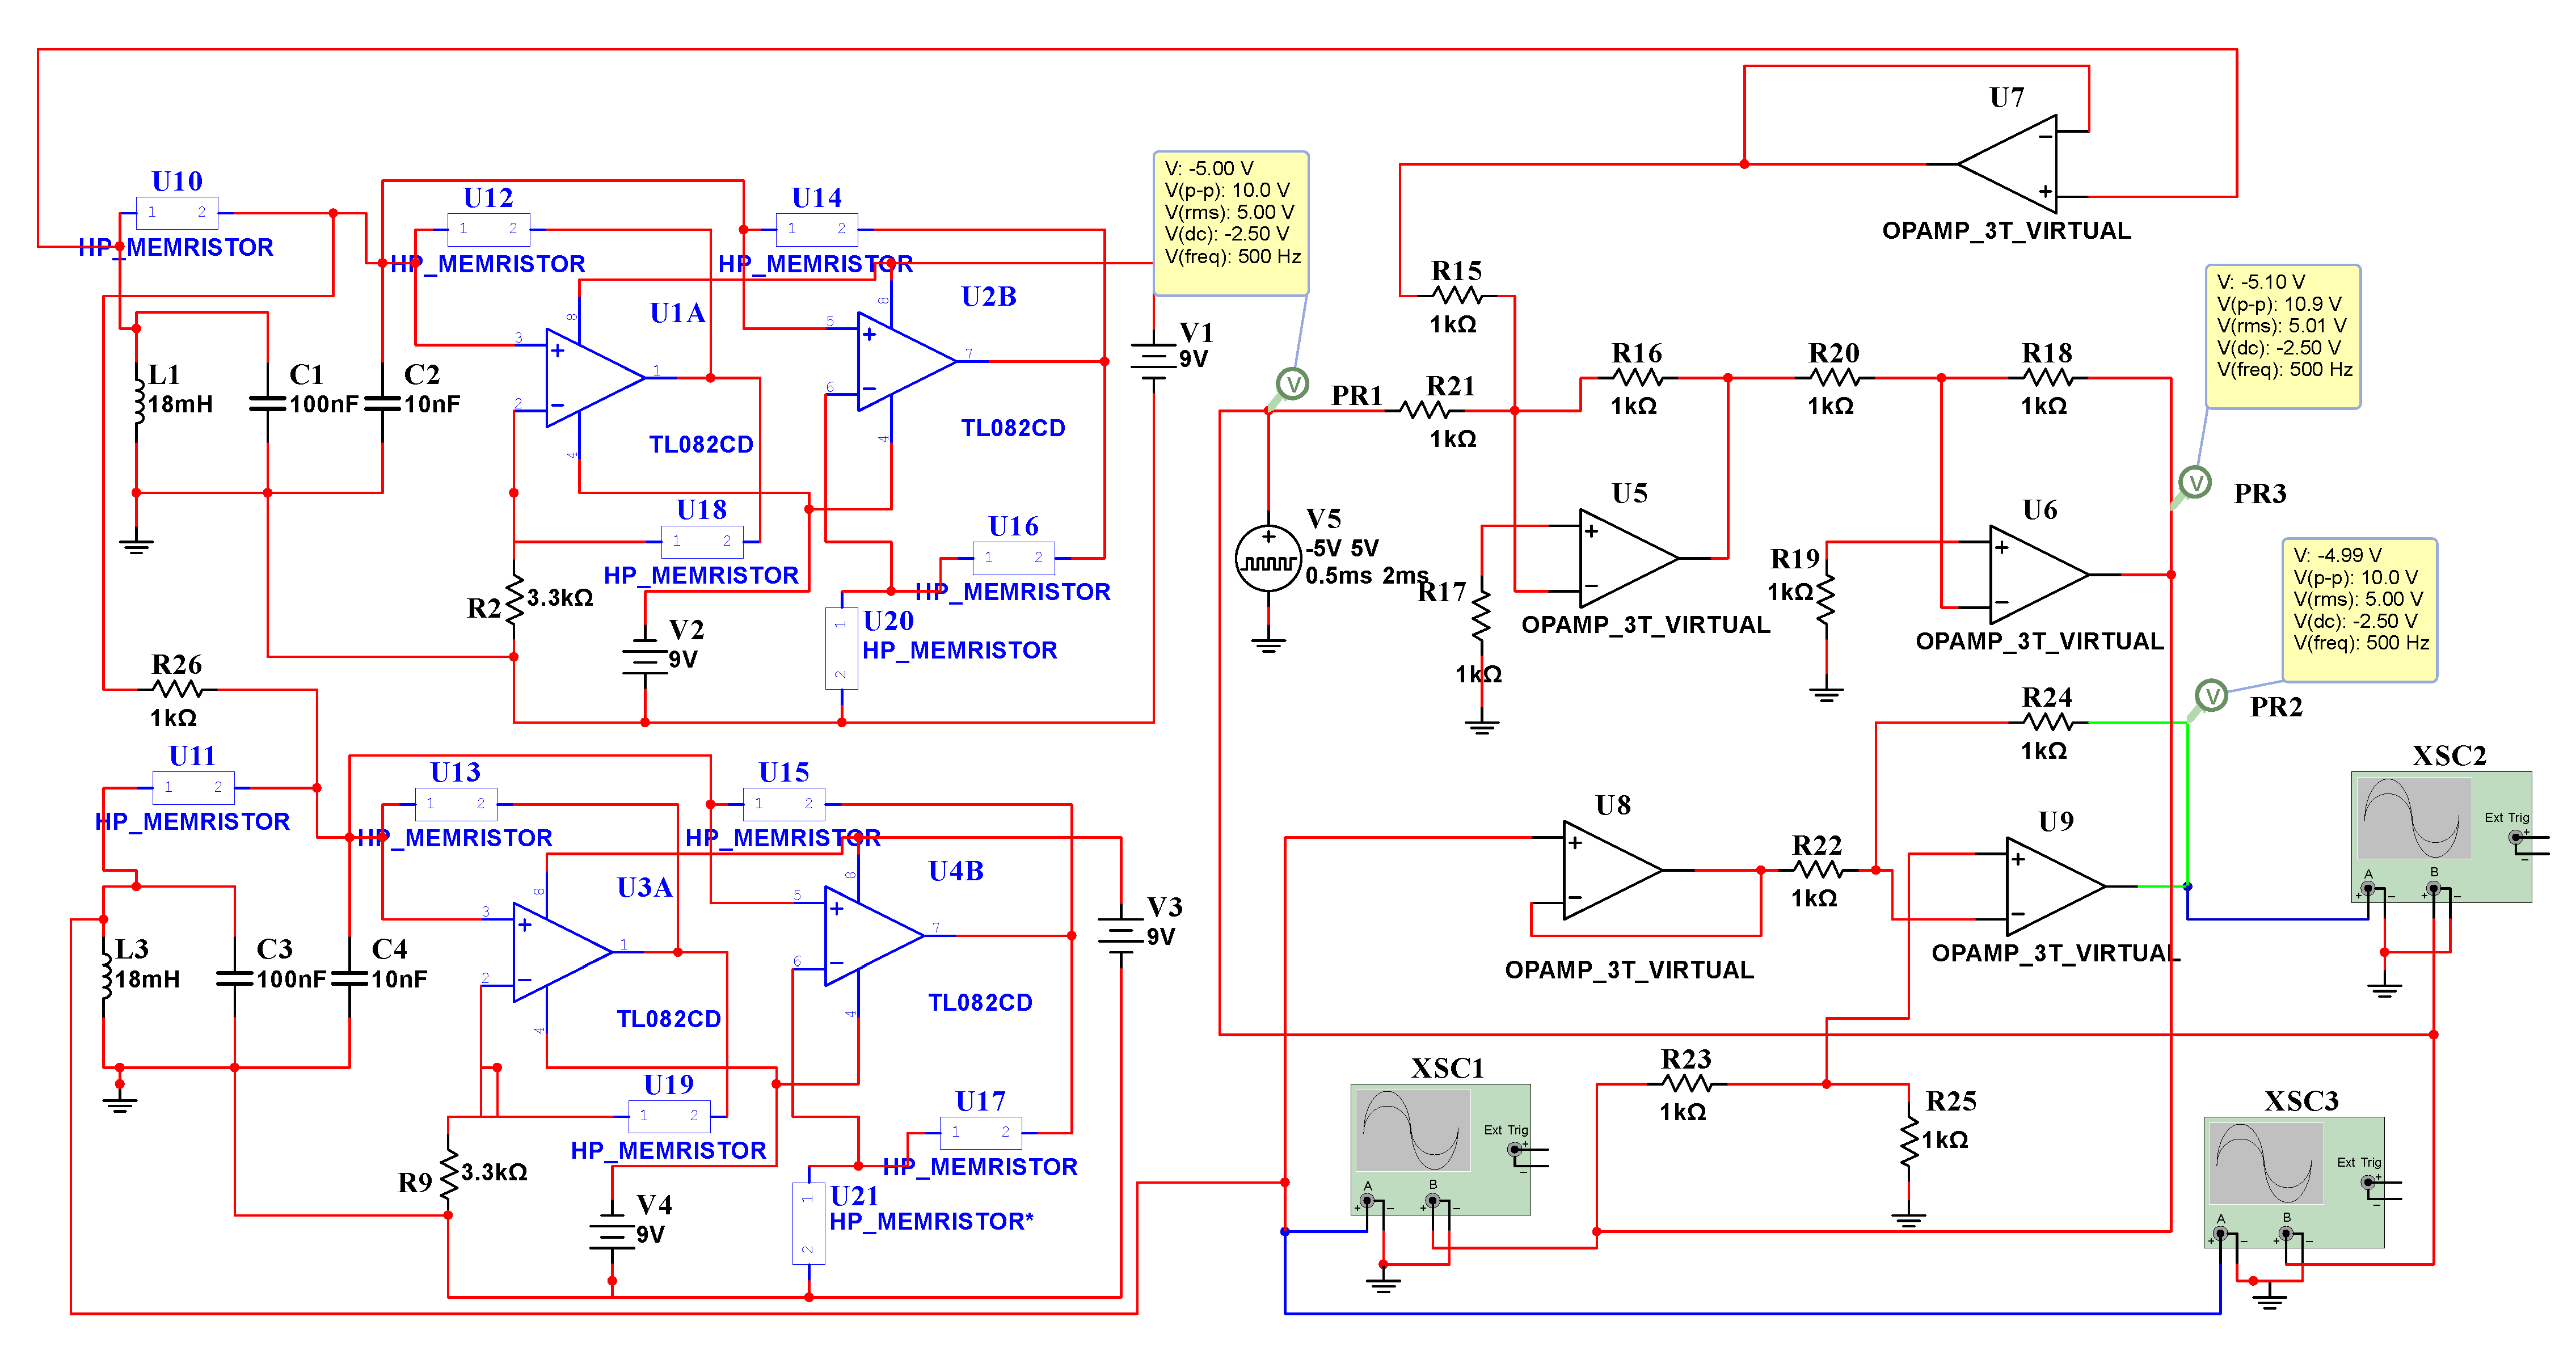
\includegraphics[width = 1\linewidth]{figs/Fig19multisim_Tx_Rx.PNG}
    \caption{Design of memristor-based Chua's chaotic circuit - non-identical transmitter and receiver}
    \label{fig:13}
\end{figure}

\begin{figure}[!t]
    \centering
    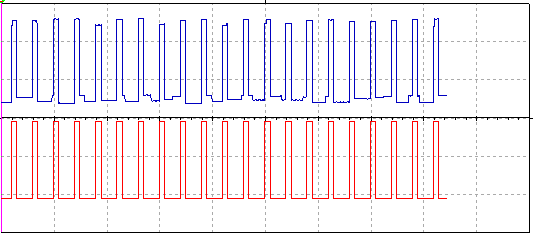
\includegraphics[width = 0.7\linewidth]{figs/Fig20x_OSC_02.PNG}
    \caption{Comparison of original message in red and decoded message in blue}
    \label{fig:14}
\end{figure}


The table below shows the values of the memristors used in the circuit of Fig. \ref{fig:13}, which remains same as Tx and Rx. Fig. \ref{fig:14} shows the original message is decoded successfully even when the circuit are non-identical. 

\begin{center}
\small
\begin{tabular}{|c c c |} 
 \hline
  &  & Memristor Parameters \\ [0.5ex] 
 \hline\hline
 Tx  & U10 & Ron=0.9K Roff=1.85K D=10N uv=10F p=1 \\ 
 \hline
 Rx & U11 & Ron=1K Roff=1.75K D=10N uv=10F p=1 \\ 
 \hline
\end{tabular}
\end{center}

\begin{center}
\small
\begin{tabular}{|c c c |} 
 \hline
 Tx & Rx & Memristor Parameters \\ [0.5ex] 
 \hline\hline
 U12 & U13 & Ron=11K Roff=22K D=10N uv=10F p=1 \\ 
 \hline
 U14 & U15 & Ron=110 Roff=220 D=10N uv=10F p=1 \\ 
 \hline
 U16 & U17 & Ron=110 Roff=220 D=10N uv=10F p=1 \\ 
 \hline
 U18 & U19 & Ron=11K Roff=22K D=10N uv=10F p=1 \\ 
 \hline
  U20 & U21 & Ron=1.1K Roff=2.2K D=10N uv=10F p=1 \\ 
 \hline
\end{tabular}
\end{center}

According to the above experiments, if the attacker discovers the correct key (i.e., the resistance of the memristors) within the range of $\Delta=0.1$, he/she may still decode the message; however, beyond this range, he/she has no luck. As a result, we take this value into account and employ the SMT attack \cite{9000113} on our proposed transceiver in Fig. \ref{fig:7}. We assume that the attacker has access to the prototyped receiver bought off the market and the transmitter design. The goal is to find the resistance of the memristors in such a way that the transmitter will be able to sync with the receiver. Each transmitter has six memristors; with $R_{max}$ set to 10K, each memristor can take $100,000$ different values resulting in $100,000^6$ cases which can be modeled with a key size of $100$ bits. We used 8GB of RAM and a 4-core processor at 2.20Ghz to run the attack. The attack, however, reports no key after 24 hours of running. This is due to the fact that the modeling of our analog logic locking circuit requires a large key space.


\section*{Discussion}

In this chapter, we presented a memristor-based chaotic transceiver designed to provide a robust defense against eavesdroppers and untrusted foundries. The efficacy of our approach lies in the creation of an extensive key space through the incorporation of memristors into the circuit, complemented by the implementation of logic locking. Validation of the proposed system was conducted through simulations in MATLAB Simulink, confirming the reliability and functionality of the memristor-based chaotic equations. This research holds particular relevance in enhancing the communication security of risk-sensitive implantable and wearable devices at the application level. By delivering a secure transceiver solution, our memristor-based chaotic system contributes significantly to fortifying the integrity of data transmission in these contexts.



\endgroup
\newpage
\fi 

\phantomsection
\addcontentsline{toc}{section}{4. CONCLUSIONS AND FUTURE WORKS}
\section*{Chapter 4 \\ CONCLUSIONS AND FUTURE WORKS }
\begingroup
\RaggedRight

In this thesis, novel methods were designed to fix the evident gaps in contemporary hardware security research. A deep learning approach, complemented by uncertainty awareness, was employed to discern and detect evolving hardware trojans. In this study we systematically addressed the case of missing modalities in the dataset, enhancing the overall quality of the proposed framework. Additionally, the thesis contributed to the field by addressing a previously overlooked evaluation metric, aiming to quantify predictions generated by machine learning methods in the intricate task of hardware Trojan detection.

Chapter 2 introduced a method to generate a quality evolving dataset using conformalized generative adversarial network. Then, we proposed an algorithm-agnostic framework called \textbf{PALETTE} to detect evolving hardware Trojans with guaranteed coverage. We also implemented a novel method for rejecting a decision by proving a calibrated explanation. \textbf{PALETTE} is efficient in detecting hardware Trojans with an assigned uncertainty quantification for each detection. Our results highlighted opportunities for researchers in related hardware security domains such as logic locking \cite{Rezaei:BreakUnroll, Rezaei:PUF, Maynard:DK-Lock, Aghamohammadi:CoLA} to rethink the application of ML-based solutions and re-construct the metrics to evaluate their methods. We do believe that there is no silver bullet for a zero-day attack, but a robust method to minimize the chances of an attack and a proactive approach to defending the attack do help.

Chapter 3 addressed the growing concern of maliciously inserted hardware Trojans into chips at various stages of production in an era where fabless manufacturing is hard to trust. Specifically, we adopted an innovative approach by utilizing generative adversarial networks to expand our dataset with two distinct representation modalities: graph and tabular. Additionally, we introduced an uncertainty-aware multimodal deep learning framework called \textit{NOODLE} for detecting hardware Trojans. We assessed our findings using both early and late fusion strategies, offering a comprehensive evaluation of our approach's efficacy. Moreover, we integrated metrics for uncertainty quantification for each prediction, enabling us to make decisions that are mindful of potential risks. The utilization of multimodality and uncertainty quantification shows great potential for addressing other critical challenges in hardware security such as logic locking \cite{Rezaei:BreakUnroll, Rezaei:PUF, Maynard:DK-Lock, Aghamohammadi:CoLA}. These contributions collectively represent a significant step forward in enhancing the security and reliability of hardware systems in the face of emerging threats.


\section*{Future Work}

Expanding upon the groundwork established in this study, prospective research should concentrate on enhancing the technical dimensions of hardware Trojan detection. This involves exploration of uncertainty quantification within multimodal deep learning frameworks, achieved by developing alternative non-conformity measures for the implemented deep learning algorithms. 

\begin{itemize}

\item First, the alternative generative models, beyond conformalized generative adversarial networks (cGANs), could be undertaken. Investigating the use of state-of-the-art generative models such as Wasserstein GANs or Progressive GANs may offer insights into improving the quality of the evolving dataset, thereby influencing the robustness of hardware Trojan detection.

\item Secondly, the \textit{NOODLE} framework, while innovative, could benefit from enhancements in uncertainty quantification methodologies. The integration of Bayesian deep learning techniques or ensemble methods might provide more accurate and calibrated uncertainty estimates, improving the reliability of the detection system in dynamic environments.
\end{itemize}

Furthermore, extending the multimodal capabilities of \textit{NOODLE} could be explored. The addition of additional modalities, such as temporal or spectral representations, could enhance the framework's ability to capture subtle variations indicative of hardware Trojans. Investigating the optimal fusion strategies for these modalities and their impact on both detection performance and uncertainty quantification is a ripe area for further exploration. Finally, the integration of the proposed frameworks into hardware security testing environments, including Hardware Security Modules (HSMs) or Field Programmable Gate Arrays (FPGAs), could be explored for real-world validation. This would involve addressing practical challenges related to resource constraints, latency, and scalability, ensuring that the proposed methods can seamlessly integrate into existing hardware security infrastructures.

\endgroup
\newpage


\iffalse 
% Appendix
\addtocontents{toc}{\setlength{\cftsecindent}{0cm}} 
\phantomsection
\addcontentsline{toc}{section}{APPENDICES}
\begin{center}
\null
\vfill
\textbf{APPENDICES}
\vfill
\newpage 
\end{center}

\begin{center}
\null
\vfill
\textbf{APPENDIX A \\ GAZE METRICS}
\vfill
\newpage 
\end{center}

\addtocontents{toc}{\setlength{\cftsecindent}{1cm}}
\phantomsection
\addcontentsline{toc}{section}{A. GAZE METRICS}
\input{appendices/a_gaze_metrics}
\newpage

\begin{center}
\null
\vfill
\textbf{APPENDIX B \\ CLASSIFIERS}
\vfill
\newpage 
\end{center}

\addtocontents{toc}{\setlength{\cftsecindent}{1cm}}
\phantomsection
\addcontentsline{toc}{section}{B. CLASSIFIERS}
\input{appendices/b_classifiers}
\newpage

\fi 

% References
\begin{center}
\null
\vfill
\textbf{REFERENCES}
\vfill
\newpage 
\end{center}

\addtocontents{toc}{\setlength{\cftsecindent}{0cm}} 
\phantomsection
\addcontentsline{toc}{section}{REFERENCES}
\renewcommand{\refname}{REFERENCES}
\printbibliography

\end{document}